% Chapters will always start on odd numbered page
\documentclass[letter,12pt]{book}

%\def \oldstuff {add old stuff}
  
\usepackage[english]{babel}
\usepackage{fancyhdr}

%% Toggle text
%\newcommand \nlptext{Show NLP text}
%\newcommand \oldstuff{Show old text}

%Toggle proofs
%\def \showproofs {If commented, many proofs will not be shown}
% See command.tex for all package imports, environments, and special commands.
\input{foundationsAppliedMathematicsLabs/command}
\usepackage{algorithm}%,algpseudocode}
\usepackage{mdframed}
\usepackage{longtable}


\cellcolor{red}

%\newcommand{\cr}[1]{\mathbf{#1}} % change to \mathbb

\newcommand{\rc}{\cellcolor{red}} % change cell color red in table
\newcommand{\hi}{\cellcolor{red}} % change cell color red in table

%\newtheorem{example}{Example}%[section]
\newtheorem{ICE}{ICE}%[section]
%\newtheorem{problem}{Problem}%[section]
%\newtheorem{solution}{Solution}%[section]

%\def\input@path{{/figures/}}
%\def\input@path{{/path/to/folder/}{/path/to/other/folder/}}

\newcounter{algsubstate}
\renewcommand{\thealgsubstate}{\alph{algsubstate}}
\newenvironment{algsubstates}
  {\setcounter{algsubstate}{0}%
   \renewcommand{\State}{%
     \stepcounter{algsubstate}%
     \Statex {\footnotesize\thealgsubstate:}\space}}
  {}


\numberwithin{equation}{section}

\graphicspath{{figures/}{optimization/figures/figures-static/}}
\usepackage{wasysym}
\newsavebox\CBox
\newcommand\hcancel[2][0.5pt]{%
  \ifmmode\sbox\CBox{$#2$}\else\sbox\CBox{#2}\fi%
  \makebox[0pt][l]{\usebox\CBox}%  
  \rule[0.5\ht\CBox-#1/2]{\wd\CBox}{#1}}

\usepackage[cc]{titlepic}
\usepackage{xcolor}
\colorlet{notgreen}{blue!50!yellow}
\newcommand{\tblue}[1]{{\color{blue} #1}}
\newcommand{\tred}[1]{{\color{red} #1}}
\newcommand{\tgreen}[1]{{\color{notgreen} #1}}

\newcommand{\code}[1]{\texttt{ #1}}
\newcommand{\complexity}[1]{{\color{red} \textit{#1}}}
\newcommand{\nphard}{\complexity{NP-Hard}}
\newcommand{\npcomplete}{\complexity{NP-Complete}}
\newcommand{\polynomial}{{\color{ansi-green} \textit{Polynomial time (P)}}}
\newcommand{\true}{\tgreen{\texttt{ true }}}
\newcommand{\false}{\tred{\texttt{ false }}}

\usepackage{scalerel}
\newcommand{\julia}{\raisebox{-.2\height}{\includegraphics[scale = 0.07]{julia-logo}}  }
\newcommand{\jupyter}{\raisebox{-.2\height}{\includegraphics[scale = 0.09]{jupyter-logo}}  }
\newcommand{\jump}{\raisebox{-.2\height}{\includegraphics[scale = 0.08]{jump-logo}}  }
\newcommand{\gurobi}{\raisebox{-.2\height}{\includegraphics[scale = 0.06]{gurobi-logo}}Gurobi  }
\newcommand{\coin}{\raisebox{-.2\height}{\includegraphics[scale = 0.2]{coin-or-logo}}  }
\newcommand{\ipopt}{\raisebox{-.2\height}{\texttt{Ipopt}}}


\usepackage{subcaption}

\def \PP{ {\mathcal{P}}}
\def \NN{ {\mathcal{N}}}
\def \II{ {\mathcal{I}}}
\def \ZZ{ {\mathcal{Z}}}
\def \SS{ {\mathcal{S}}}
\def \FF{ {\mathcal{F}}}
\def \CC{ {\mathcal{C}}}
\def \nn{ {\mathbb{N}}}
\def \R{ {\mathbb{R}}}
\def \Z{ {\mathbb{Z}}}
\def \Q{ {\mathbb{Q}}}
\def \cc{ {\mathbb{C}}}

\DeclareMathOperator{\dom}{dom}
\DeclareMathOperator{\cl}{cl}
\DeclareMathOperator{\intr}{intr}

\def \rank{\textup{rank}}
\def \size{\textup{size}}
%\def \dist{\textup{dist}}
\def \sign{\textup{sign}}
\def \deg{\textup{deg}}
\def \conv{\textup{conv}}
\def \cone{ {\textup{cone}}}
\def \supp{\textup{supp}}
\def \int{ {\textup{int}}}
\def \rc{\textup{rec.cone}}
\def \ri{\textup{rel.int}}
\def \rb{ {\textup{rel.bd}}}
\def \bd{ {\textup{bd}}}
\def \ls{\textup{lin.space}}
\def \tq{{\,:\,}}
\def \aff{{\textup{aff}}}
\def \one{\mathbb{1}}
\def \st{ \text{ s.t. }}

\def \BQP{\mathrm{BQP}}
\def \xLP{x^{\mathrm{LP}}}
\DeclareMathOperator    \argmin         {arg\,min}
%\DeclareMathOperator    \argmax         {arg\,max}


%\newcounter{example}
\newcounter{general}

  % Test Environment
  \newcounter{exo}
\makeatletter
\newenvironment{exo}[1]%
{\refstepcounter{exo}%
\protected@edef\@currentlabelname{Exercise \theexo: #1}% addition here
\vspace{0.5cm}\noindent
{\large\bfseries{Exercise \theexo~: #1} \par}
{\par\vspace{0.5cm}}}
\makeatother

\newcounter{codeCell}
\makeatletter
\newenvironment{codeCell}%
{\refstepcounter{codeCell}%
\protected@edef\@currentlabelname{Code}% addition here
{}
%{\large\bfseries{Exercise \theexo~: #1} \par}
{}}
\makeatother

% General environment
\newenvironment{general}[2]
  {\par\medskip
   %\refstepcounter{exo}%
  \protected@edef\@currentlabelname{#1}
   \begin{framed}
   \begingroup\color{black}%
   \textbf{#1: }\ignorespaces
   \par #2
   \par}
 {\endgroup\end{framed}
  \medskip}
  

 % Example Environment
  \newenvironment{optexample}
  {\par\medskip
  \refstepcounter{exo}%
  \protected@edef\@currentlabelname{Example \theexo}
   \begin{framed}
   \begingroup\color{blue}%
   \textbf{Example \theexo: }\ignorespaces}
 {\endgroup\end{framed}
  \medskip}
  
  
  % Example with code Environment
   \newenvironment{examplewithcode}[2]
  {\par\medskip
   \refstepcounter{exo}%
  \protected@edef\@currentlabelname{Example \theexo}
  \begin{center}
 \rule{\textwidth}{0.4pt}\\
 \vspace{-0.2cm}
 \rule{\textwidth}{0.4pt}
 \end{center}
   %\begin{framed}
   \begingroup\color{black}%
   \textbf{Example: #1}
   \hfill \protect\href{#2}{Gurobipy}% code link somehow
    \ignorespaces
    \par}
 { \endgroup
 %\end{framed}
   \begin{center}
 \rule{\textwidth}{1.8pt}
 \end{center}
  \medskip}
  
    % Example with all code Environment
   \newenvironment{examplewithallcode}[4]
  {\par\medskip
   \refstepcounter{exo}%
  \protected@edef\@currentlabelname{Example \theexo}
   \begin{framed}
   \begingroup\color{black}%
   \textbf{Example: #1}
   \hfill \protect\href{#2}{ \ Excel \ }\protect\href{#3}{ \ PuLP \ }\protect\href{#4}{\ Gurobipy \ }% code link somehow
    \ignorespaces
    \par}
 { \endgroup
 \end{framed}
  \medskip}
  
    % Example without code Environment
   \newenvironment{examplewithoutcode}[2]
  {\par\medskip
   \refstepcounter{exo}%
  \protected@edef\@currentlabelname{Example \theexo}
   \begin{framed}
   \begingroup\color{black}%
   \textbf{Example: #1}
    \ignorespaces
    \par}
 { \endgroup
 \end{framed}
  \medskip}
  

\newcommand{\floor}[1]{\lfloor #1 \rfloor}
\newcommand{\ceil}[1]{\lceil #1 \rceil}


\newcommand{\mathup}[1]{#1}
\newcommand{\NP}{\text{NP}}
\newcommand{\coNP}{\text{coNP}}
  
\input{optimization/preamble0}
%%% BibLaTeX setup --> see also
%%% /open-optimization-bibliography/test/bibliography-biblatex.tex.

\usepackage{csquotes}   % to work around a bug in pre-2018 biblatex, https://github.com/plk/biblatex/issues/737
\usepackage[backend=biber,giveninits=true,maxnames=100,maxcitenames=5,sorting=nyt,backref=true]{biblatex}
\addbibresource{../../../open-optimization-bibliography/bib/references.bib}
\addbibresource{../../figures/figures-static/00_METADATA.bib}

\DeclareRobustCommand\footnotetextmetadata[1]{%
  \footnotetext{\citetitle*{#1}, from \citeurl{#1}.
    \citeauthor{#1}, \citedate{#1}.
  }
}

\usepackage{xargs}
\newcommandx{\refincludefigurestatic}[3][1=\relax,2={width=.4\linewidth},usedefault]{%
  \begin{figure}[t]%
    \centering%
    \includegraphics[#2]{../../figures/figures-static/#3}%
    \caption{%
      \ifx#1\relax % Caption from TITLE field in .bib
      \citetitle*{#3}%
      \else        % Caption provided as an argument to the macro
      #1%
      \fi%
      \protect\footnotemark}%
    \label{fig:#3}%
  \end{figure}%
  \autoref{fig:#3}\footnotetextmetadata{#3}%
}

%%% Local Variables:
%%% mode: latex
%%% TeX-master: "open-optimization/open-optimization"
%%% End:

\input{preamble-jupyter.tex}

\usepackage{pdfpages}

\usepackage{booktabs}

\graphicspath{ {./images/}{images/}{optimization/multi-objective/images/} }
% For the font
\usepackage{mathptmx}
%\usepackage{roboto} %%for Lyryx Icon font
\usepackage[T1]{fontenc}
\usepackage[EULERGREEK]{sansmath}

% Various math packages
\usepackage{amsmath,amsfonts,amsthm,amssymb}

% Make it look more like the Word docs
%\setlength{\parskip}{\baselineskip}
%\setlength{\parindent}{0pt}

% Simple arithmetic
\usepackage{calc}

% For colouring various things
\usepackage{xcolor}

% Colored tables and other nice enhancements
\usepackage{tabu}

% Conditional statements
\usepackage{ifthen}

% Page layout
\ifthenelse{\equal{\detokenize{interior}}{\jobname}}{
	\usepackage[headheight=15pt,top=1in, bottom=0.75in, outer=0.65in, inner=0.85in]{geometry}
        % \usepackage[headheight=15pt,top=1in, bottom=0.1in, outer=0.75in, inner=1.25in]{geometry}
}{
  \usepackage[headheight=15pt,top=1in, bottom=0.75in, outer=0.75in, inner=0.75in]{geometry}
  %\usepackage[headheight=15pt,top=1in, bottom=0.1in, outer=1in, inner=1in]{geometry}
}

% Captions for objects
\usepackage[format=hang,font=bf]{caption}
  
% Additional commands for simple LaTeX drawings
\usepackage{eepic}

% For multicolumn cells in text
\usepackage{multicol}

% Standard package for creating indexes
\usepackage{makeidx} 

% If you want to include postscript graphics
\usepackage{graphicx}

% For including eps graphic files
\usepackage{epsfig}

% Additional features for lists
\usepackage{mdwlist}

% Coloured titlepage setup
\usepackage{afterpage}
\usepackage{pagecolor}

% Hyperlinks
\usepackage{hyperref}


% To insert df page (only open text distribution project)
%\usepackage{pdfpages}

% Creates coloured boxes
\usepackage{tcolorbox}
\tcbuselibrary{theorems,breakable}

% Draw frames around text
\usepackage[framemethod=tikz]{mdframed}
\mdfsetup{skipabove=\topskip,skipbelow=\topskip}

% To remove headers and footers from truly empty pages
\usepackage{emptypage}

% Draw images and figures
\usepackage{rotating}
\usepackage{tikz}
\usetikzlibrary{calc,intersections,shapes.callouts}
\usetikzlibrary{decorations.text}
\usetikzlibrary{positioning}
\usetikzlibrary{decorations.pathreplacing}
\usetikzlibrary{shadows}
\usetikzlibrary{backgrounds}
\usepackage{circuitikz}
\tikzstyle arrowstyle=[scale=2.5]
\tikzstyle directed=[postaction={decorate,decoration={markings,
    mark=at position .65 with {\arrow[arrowstyle]{latex}}}}]
\tikzstyle directed1=[postaction={decorate,decoration={markings,
    mark=at position .99 with {\arrow[arrowstyle]{latex}}}}]   
\tikzstyle{vertex}=[circle,fill=black!25,minimum size=20pt,inner sep=0pt]

\definecolor{ocre}{RGB}{243,102,25} % Define the orange color used for highlighting throughout the book

% Thew following passes on paperheight to ps2pdf... bug fix  
\pdfpageheight=\paperheight 

% For plotting data
\usepackage{pgfplots}
\usepackage{pgfplotstable}

% For fancy headers!
\usepackage{fancyhdr}

% Used for creating EOC questions with corresponding solutions at the end of the textbook
\usepackage{answers}

% fancy section headers, sc for small caps, prevent titles from being stranded on previous page
\usepackage[explicit,sc,nobottomtitles]{titlesec}


% Inputs information regarding book Title, Authors, Version and Revision
\input aFirstCourseLinearAlgebra/frontmatter/bookinfo.txt

% Inputs information regarding Institution,Course Code, Name, Session and Section (for adapted text)
%\input aFirstCourseLinearAlgebra/courseInfo.txt

% Lyryx Math Style
\usepackage{aFirstCourseLinearAlgebra/LyryxMathStyle}

% Lyryx Linear Algebra Style 
\usepackage{aFirstCourseLinearAlgebra/LyryxLinAlgStyle}


\renewcommand{\b}{\mathbf{b}}
\renewcommand{\x}{\mathbf{x}}
\renewcommand{\c}{\mathbf{c}}
\renewcommand{\0}{\mathbf{0}}
\renewcommand{\u}{\mathbf{u}}

%% Print Setup
\newlength{\coverwidth}
\newlength{\frontsideleft}
\newlength{\pagethickness}

%%set page number of interior
\newcommand{\numpages}{604}

% Color interior
\setlength{\pagethickness}{0.0025in}

% B+W Interior
%\setlength{\pagethickness}{0.002252in}

% TODO: Is there a way to automatically calculate the dimensions of the print-cover? 
%%%%%%%%%%%%%%%%%%%%%%%%%%%%%%%%
%
% PRINT COVER GEOMETRY CALCULATIONS
%
% % %
%%% Here are the calculations from createspace:
% 
% Spine width: --> black+white interior is 0.002252in * page count
%              --> colour interior is 0.0025in * page count
%
% Spine: allow for 0.0625" variance on either side of the fold lines for your cover.
%
% Bleed: 0.125 * 2  (needed on all 4 outside edges of PDF, but not spine)
%
% Safe zone: Text and images must be at least .125" inside the trim lines to ensure
%            that no live elements are cut during the bookmaking process.
%
% Minimum Cover Width: Bleed + Back Cover Trim Size + Spine Width + Front Cover Trim Size + Bleed
%
% 
% For 108 pages in colour: (exclude front and back cover - 2 pages)
%
% paper width = 0.125 + 8.5 + (0.0025 * 108) + 8.5 + 0.125 = 17.52in
% paper height = 11 + (2 * 0.125) = 11.25in
%
%                paper size - safe zone		(layoutsize)
% layout width = 8.5 - (.125 * 2)
% layout height = 11 - (.125 * 2)
%
%                   bleed + left side + spine + safe zone
% layout offset x = 0.125 + 8.5 + (0.0025 * 108) + 0.125 = 9.02in
%                   bleed + safe zone
% layout offset y = 0.125 + 0.125 = 0.25in
%
% spine width:	0.002252 * 360 = 0.81072in B&W
% 				0.0025 * 360 = 0.9in colour
%
%
% HOWEVER this will leave space for headers/footers/marginal notes/etc
%
% So we want to tweak the body size to be something nice, such as layoutsize minus 1/2 inch on each side for margins
%
%% LULU DIMENSIONS
%
%From Lulu:
%Spine width = 0.419cm
%Spine begins = 21.905cm from the left
%Total cover width = 44.229cm X 28.571cm 

%CreateSpace
%\setlength{\coverwidth}{0.125in + 8.5in + (\pagethickness * \numpages) + 8.5in + 0.125in}
%\setlength{\frontsideleft}{0.125in + 8.5in + (\pagethickness * \numpages) + 0.125in}

%Lengths from LULU for samples 2017-01-16
\setlength{\coverwidth}{44.229cm}
\setlength{\frontsideleft}{21.905cm+0.419cm+0.3cm} %Spine begins + Spine width +safe zone

% Options showframe, showcrop, and verbose can be used for debugging
\ifthenelse{\equal{\detokenize{print-cover}}{\jobname}}{
%   \geometry{papersize={\coverwidth,28.571cm},layoutsize={21cm,27.3cm},layoutoffset={\frontsideleft,0.6cm},body={18.4cm,24.7cm}}
	\geometry{papersize={\coverwidth,28.571cm},layoutsize={21.3cm,27.3cm},layoutoffset={\frontsideleft,0.3cm},body={18.4cm,24.7cm}}
}{
	% No change in geometry for regular pdf
}

%To create index
\makeindex


 \title{ \textbf{Mathematical Programming and\\ Operations Research}\\ Modeling, Algorithms, and Complexity\\
 Examples in Python and Julia\\
 (Work in progress)}
  \author{Edited by: Robert Hildebrand\\[1ex]
 Contributors:
 Robert Hildebrand, Laurent Poirrier \\
% $\bullet$ ???\hspace{5cm} \\
%  $\bullet$ ???\hspace{5cm} \\
%   $\bullet$ ???\hspace{5cm} \\t
%   $\bullet$ ???\hspace{5cm} \\
%   $\bullet$ ???\hspace{5cm} \\
%   $\bullet$ ???\hspace{5cm} \\
%    $\bullet$ ???\hspace{5cm}
  }

%%% Local Variables:
%%% mode: latex
%%% TeX-master: "open-optimization"
%%% End:
 
%By Kevin Cheung
%The book is licensed under the
%\href{http://creativecommons.org/licenses/by-sa/4.0/}{Creative Commons
%Attribution-ShareAlike 4.0 International License}.
%
%This file has been modified by Robert Hildebrand 2020.  
%CC BY SA 4.0 licence still applies.



\def\lt{<}
\def\gt{>}
\newcommand{\ssep}{~:~}
\newcommand{\T}{\mathsf{T}}

\newcommand{\mm}[1]{\mathbf{#1}}

\renewcommand{\vec}[1]{\mathbf{#1}}

\graphicspath{{aFirstCourseLinearAlgebra/},{lineqlpbook/},{optimization/figures/figures-static/},{Christopher_Griffin_Penn_State_University/}}



\usetikzlibrary{arrows.meta,positioning}

\usepackage{todonotes}


\begin{document}


\input{optimization/LP-front-matter.tex}



% Title page
%\ifthenelse{\equal{\detokenize{print-cover-front}}{\jobname}}{
%	\pagestyle{empty}
%	\input frontmatter/titlepage
%}{
%\ifthenelse{\equal{\detokenize{print-cover}}{\jobname}}{
%	\pagestyle{empty}
%	\input frontmatter/titlepage
%}{
%	\raggedbottom
%	\allowdisplaybreaks
%	\frontmatter
%
%\ifthenelse{\equal{\detokenize{interior}}{\jobname}}{
%	% Skip title page for interior
%}{
%	\input frontmatter/titlepage.tex
%	\cleardoublepage
%}
\input preface.tex
%	\begin{center}
%\href{https://pixabay.com/illustrations/under-construction-construction-sign-2408060/}{\includegraphics[scale = 0.1]{optimization/figures/under-construction-2408060_1280}}
%\end{center}

%This entire book is a working manuscript. 
%
%\begin{center}
%\fontsize{14pt}{16pt}\selectfont\textcolor{titletextcolour}{\textbf{MAJOR ACKNOWLEDGEMENTS}}
%\end{center}
%
%I would like to acknowledge that substantial parts of this book were borrowed under a CC-BY-SA license.   These substantial pieces include:
%\begin{itemize}
%\item "A First Course in Linear Algebra" by Lyryx Learning (based on original text by Ken Kuttler).   A majority of their formatting was used along with selected sections that make up the appendix sections on linear algebra. We are extremely grateful to Lyryx for sharing their files with us.  They do an amazing job compiling their books and the templates and formatting that we have borrowed here clearly took a lot of work to set up.  Thank you for sharing all of this material to make structuring and formating this book much easier! See subsequent page for list of contributors.
%\item "Foundations of Applied Mathmatics" with many contributors.  See \url{https://github.com/Foundations-of-Applied-Mathematics}.  Several sections from these notes were used along with some formatting.  Some of this content has been edited or rearranged to suit the needs of this book.  This content comes with some great references to code and nice formatting to present code within the book.   See subsequent page with list of contributors.
%\item "Linear Inequalities and Linear Programming" by 
%Kevin Cheung.  See \url{https://github.com/dataopt/lineqlpbook}.  These notes are posted on GitHub in a ".Rmd" format for nice reading online.  This content was converted to \LaTeX using Pandoc.    These notes make up a substantial section of the Linear Programming part of this book.
%\item Linear Programming notes by Douglas Bish.  These notes also make up a substantial section of the Linear Programming part of this book.
%\end{itemize}
%
%I would also like to acknowledge Laurent Porrier and Diego Moran for contributing various notes on linear and integer programming. 



% Revision  
	%\setcounter{page}{1}
\thispagestyle{empty}


\vspace{-3em}
%\begin{center}
%	
\includegraphics[width=.4\textwidth]{figures/LyryxLogo.eps}\footnote{This book was not produced by Lyryx, but this book has made substantial use of their open source material from "A First Course in Linear Algebra".  We leave this page in here as a tribute to Lyryx for sharing their content.}
%\end{center}

\vspace{-2em}

%\begin{center}
% {\fontsize{24pt}{22pt}\selectfont \textcolor{titletextcolour}{\booksubtitle\;\booktitle}} \\ 
%{\fontsize{16pt}{20pt}\selectfont \textcolor{titlemainbgcolour}{an Open Text}} %{\fontsize{16pt}{20pt}\selectfont\textcolor{titlemainbgcolour}{by \bookauthor}}
%
%\medskip

%\fontsize{14pt}{20pt}\selectfont\textcolor{titletextcolour}{\textbf{Version\,\version \enskip---\enskip Revision\,\revision}}
%\end{center}

\setlength{\parskip}{0pt}

\begin{center}
\fontsize{12pt}{14pt}\selectfont\textcolor{titletextcolour}{\textbf{Revision History \\ \smallskip  Current Revision: Version\, 2020%\version 
\enskip---\enskip Revision\,\revision }}
\end{center}

{\footnotesize

\begin{center}
Substantial open source content has been added to the book to fill out various sections.   All content is still released under a CC-BY-SA 4.0 license.
\end{center}

%%with package enuitem can use [leftmargin=*] after \begin{itemize}
\begin{tabu}{p{3em} X[j,m]} %\hline
%Revision & \centering{Author: Significant Changes} \\  
\hline
\textcolor{titletextcolour}{2020} \textcolor{titletextcolour}{A} & \begin{itemize} \item R. Hildebrand: Added content on Linear Algebra and Linear Programming, and updated other content.    \end{itemize} \\  \hline
2019 A &  \begin{itemize} \item R. Hildebrand: First version of the book was created. \end{itemize} \\ \end{tabu}
\medskip
}


\setlength{\parskip}{\baselineskip}



	\cleardoublepage

%\end{document} %to compile only the front matter

% Table of Contents
	\phantomsection
	\addcontentsline{toc}{chapter}{Contents} %Adds contents to the table of contents itself
	\setlength{\parskip}{3.5pt} % alter vertical space in subsequent contents. Can alter this value to adjust TOC to fit nicely on page and prevent widows/orphans, careful that this will affect the entire text. 
	\addtocontents{toc}{\protect\hypertarget{toc}{}}
	\tableofcontents
	\cleardoublepage
	
	\mainmatter
	
%LOAD COURSE CONTENT
	%\input courseSetup.tex
	
%%%%%%%%%%%%%%%
%%% Course Content %%%
%%%%%%%%%%%%%%%

%LOAD CHAPTERS / SECTIONS / SUBSECTIONS IN DESIRED ORDER





\chapter{Resources and Notation}
\todoChapter{ {\color{gray} 90\% complete. Goal 80\% completion date: Done}\\
Notes: }
Here are a list of resources that may be useful as alternative references or additional references.

\paragraph{\textbf{Free notes and textbooks}}
\begin{itemize}
\item \href{https://oer.avu.org/handle/123456789/780}{Linear Programming by K.J. Mtetwa, David}
\item \href{http://www.optimization-online.org/DB_FILE/2013/12/4161.pdf}{A first course in optimization by Jon Lee}
\item \href{https://people.inf.ethz.ch/fukudak/lect/opt2011/aopt11note1.pdf}{Introduction to Optimizaiton Notes by Komei Fukuda}
\item \href{https://web.stanford.edu/~boyd/cvxbook/}{Convex Optimization by Bord and Vandenberghe}
\item  \href{http://math.mit.edu/~goemans/18310S15/lpnotes310.pdf}{LP notes of Michel Goemans from MIT }
\item \href{https://www.springer.com/gp/book/9783540306979}{Understanding and Using Linear Programming - Matousek and G\"artner} [Downloadable from Springer with University account]
\item \href{https://rd.springer.com/book/10.1007/978-1-4471-5577-5}{Operations Research Problems
Statements and Solutions
-
Ra\'ul PolerJosefa Mula Manuel D\'iaz-Madro\~nero} [Downloadable from Springer with University account]
\end{itemize}
\paragraph{\textbf{Notes, books, and videos by various solver groups}}
\begin{itemize}
\item \href{https://www.aimms.com/english/developers/resources/manuals/optimization-modeling/}{AIMMS Optimization Modeling}
\item \href{https://www.lindo.com/index.php/ls-downloads?id=112:lingo-documentation&catid=82}{Optimization Modeling with LINGO by Linus Schrage} 
\item \href{https://ampl.com/resources/the-ampl-book/chapter-downloads/}{The AMPL Book}
\item \href{https://learning.oreilly.com/library/view/microsoft-excel-2019/9781509306091/?ar}{Microsoft Excel 2019 Data Analysis and Business Modeling, Sixth Edition, by Wayne Winston} - Available to read for free as an e-book through Virginia Tech library at Orielly.com.
\item \href{https://www.microsoftpressstore.com/store/microsoft-excel-2019-data-analysis-and-business-modeling-9781509305889}{Lesson files for the Winston Book}
\item \href{https://www.xelplus.com/excel-solver-example/}{Video instructions for solver and an example workbook}

\item \href{https://www.youtube.com/playlist?list=PLgA4wLGrqI-ll9OSJmR5nU4lV4_aNTgKx}
{\includegraphics[scale = 0.15]{youtube-OR-course}}
\end{itemize}

\paragraph{\textbf{Gurobi Links}}
\begin{itemize}
\item Go to \url{https://github.com/Gurobi} and download the example files.
\item \href{https://pages.gurobi.com/rs/181-ZYS-005/images/Management%20Paper_5%20Essential%20Ingredients%20for%20Optimization%20Success.pdf}{Essential ingredients}
\item \href{https://www.gurobi.com/resource/mathematical-programming-tutorial-linear-programming/}{Gurobi Linear Programming tutorial}
\item \href{https://www.gurobi.com/resource/tutorial-mixed-integer-linear-programming/}{Gurobi tutorial MILP}
\item \href{https://www.gurobi.com/resource/python-i-webinar/}{GUROBI - Python 1 - Modeling with GUROBI in Python}
\item \href{https://www.gurobi.com/resource/python-ii-webinar/}{GUROBI - Python II: Advanced Algebraic Modeling with Python and Gurobi}
\item \href{https://www.gurobi.com/resource/python-iii-webinar/}{GUROBI - Python III: Optimization and Heuristics}
\item \href{https://www.gurobi.com/wp-content/uploads/2018/12/python-3-webinar-materials.zip}{Webinar Materials}
\item \href{https://www.gurobi.com/resources/?category-filter=tutorials}{GUROBI Tutorials}
\end{itemize}

\paragraph{\textbf{How to prove things}}
\begin{itemize}
\item \href{https://open.umn.edu/opentextbooks/textbooks/book-of-proof}{Hammack - Book of Proof}
\end{itemize}

\paragraph{\textbf{Statistics}}
\begin{itemize}
\item\href{https://d3bxy9euw4e147.cloudfront.net/oscms-prodcms/media/documents/IntroductoryStatistics-OP_LXn0jei.pdf}{Open Stax - Introductory Statistics}
\end{itemize}

\paragraph{\textbf{Linear Algebra}}
\begin{itemize}
\item\href{http://linear.ups.edu/html/fcla.html}{Beezer - A first course in linear algebra}
\item\href{https://github.com/selinger/linear-algebra}{Selinger - Linear Algebra}
\item\href{https://www.math.ucdavis.edu/~linear/linear-guest.pdf}{Cherney, Denton, Thomas, Waldron - Linear Algebra}
%CC BY SA NC
\end{itemize}

\paragraph{\textbf{Real Analysis}}
\begin{itemize}
\item\href{http://www.trillia.com/zakon-analysisI.html}{Mathematical Analysis I
by Elias Zakon}
\end{itemize}

\paragraph{\textbf{Discrete Mathematics, Graphs, Algorithms, and Combinatorics}}
\begin{itemize}
\item \href{http://discrete.openmathbooks.org/dmoi3.html}{Levin - Discrete Mathematics - An Open Introduction, 3rd edition}
\item \href{https://github.com/oscarlevin/discrete-book}{Github - Discrete Mathematics: an Open Introduction} CC BY SA
\item \href{http://www.rellek.net/book/frontmatter-1.html}{Keller, Trotter - Applied Combinatorics} (CC-BY-SA 4.0)
\item \href{https://github.com/mitchkeller/applied-combinatorics}{Keller - Github -  Applied Combinatorics}
\end{itemize}

\paragraph{\textbf{Programming with Python}}
\begin{itemize}
\item\href{https://open.umn.edu/opentextbooks/textbooks/a-byte-of-python}{A Byte of Python}
\item\href{https://github.com/swaroopch/byte-of-python}{Github - Byte of Python} (CC-BY-SA)
\end{itemize}



Also, go to \url{https://github.com/open-optimization/open-optimization-or-examples} to look at more examples.


\documentclass[../open-optimization/open-optimization.tex]{subfiles}

%%%%%%%%%
\begin{document}
%%%%%%%%%

\chapter*{Introduction}s
\import{../open-optimization-sections/}{Notation.tex}
%\import{../open-optimization-sections/}{references-and-videos.tex}


%%%%%%%%%
\end{document}
%%%%%%%%%
\input{optimization/introductionNotation}

% Copyright 2020 by Robert Hildebrand
%This work is licensed under a
%Creative Commons Attribution-ShareAlike 4.0 International License (CC BY-SA 4.0)
%See http://creativecommons.org/licenses/by-sa/4.0/

%\documentclass[../open-optimization/open-optimization.tex]{subfiles}
%
%\begin{document}

\chapter{Mathematical Programming}

\todoChapter{ {\color{gray} 50\% complete. Goal 80\% completion date: August 20}\\ 
Notes: This chapter is meant to be an introduction to all the types of deterministic problems that we might discuss.  It should list many applications, have a number of pictures, and describe how and where these types of problems are used.  }

\todo[inline]{Add intro that explains the format of problems, i.e., what the complexity comment means in each problem and add pointer to section on computational complexity.}
\todo[inline]{
Add discussion of Optimization, Operations Research, and Mathematical Programming including background and applications.   
Also, give an introduction to the content in this book, what you will learn by working though the book, and why this book is interesting and different from other sources.}

\begin{outcome}
\begin{itemize}
\item Identify reasons for studying operations research
\item Define "Mathematical Programming"
\item Learn about different applications of the tools in this book
\item Explore the different types of optimization models and what types we will see in this book
\end{itemize}
\end{outcome}
\section{Why study operations research?}

\section{What is Mathematical Programming?}

\section{Applications}


\section{Types of Optimization problems}
We will state main general problem classes to be associated with in these notes.  These are Linear Programming (LP), Mixed-Integer Linear Programming (MILP), Non-Linear Programming (NLP), and Mixed-Integer Non-Linear Programming (MINLP).  


%\begin{center}
%\includegraphics[scale = 0.5]{problem-class-diagram}\footnote{Diagram by Diego Moran}
%\end{center}

\includefigurestatic[][width = 1\linewidth][h]{problem-class-diagram}

Along with each problem class, we will associate a complexity class for the general version of the problem.  See \autoref{sec:complexity} for a discussion of complexity classes.  Although we will often state that input data for a problem comes from $\R$, when we discuss complexity of such a problem, we actually mean that the data is rational, i.e., from $\Q$, and is given in binary encoding.

\section{Linear Programming (LP)}
\todo[inline]{Describe applications and andd images}
Some linear programming background, theory, and examples will be provided in \autoref{sec:LP-background}.
\begin{general}{Linear Programming (LP)}{\polynomial}
%\label{general:LP}
Given a matrix $A \in \R^{m\times n}$, vector $b \in \R^m$ and vector $c \in \R^n$, the \emph{linear programming} problem is
\begin{equation}
\label{eq:LP}
\begin{split}
\max \quad & c^\top x\\
\st  \quad & Ax \leq b\\
& x \geq 0
\end{split}
\end{equation}
\end{general}

Linear programming can come in several forms, whether we are maximizing or minimizing, or if the constraints are $\leq, =$ or $\geq$.   One form commonly used is \emph{Standard Form} given as 
\begin{general}{Linear Programming (LP) Standard Form}{\polynomial}
Given a matrix $A \in \R^{m\times n}$, vector $b \in \R^m$ and vector $c \in \R^n$, the \emph{linear programming} problem in \emph{standard form} is
\begin{equation}
\label{eq:standardLP}
\begin{split}
\max \quad & c^\top x\\
\st  \quad & Ax = b\\
& x \geq 0
\end{split}
\end{equation}
\end{general}
\todo[inline]{Can shrink figure if there are not a lot of numbers of greek letters involved.}
\refincludefigurestatic[Linear programming constraints and objective.][scale = 0.2][h]{wiki/File/linear-programming.png}

\todo[inline]{Move this to simplex chapter}
\begin{exercise}
\label{exercise:LPconversion}
Start with a problem in form given as \eqref{eq:LP} and convert it to standard form \eqref{eq:standardLP} by adding at most $m$ many new variables and by enlarging the constraint matrix $A$ by at most $m$ new columns.
\end{exercise}
\section{Mixed-Integer Linear Programming (MILP)}
Mixed-integer linear programming will be the focus of Sections \ref{sec:IP-formulations},\ref{sec:exponential-IP-forumulations}, \ref{sec:IP-algorithms}, and \ref{sec:IP-heuristics}.
Recall that the notation $\Z$ means the set of integers and the set $\R$ means the set of real numbers.  The first problem of interest here is a \emph{binary integer program} (BIP) where all $n$ variables are binary (either 0 or 1).

\begin{general}{Binary Integer programming (BIP)}{\npcomplete}
Given a matrix $A \in \R^{m\times n}$, vector $b \in \R^m$ and vector $c \in \R^n$, the \emph{binary integer programming} problem is
\begin{equation}
\label{eq:BIP}
\begin{split}
\max \quad & c^\top x\\
\st  \quad & Ax \leq b\\
& x \in \{0,1\}^n
\end{split}
\end{equation}
\end{general}
A slightly more general class is the class of \emph{Integer Linear Programs} (ILP).  Often this is referred to as \emph{Integer Program} (IP), although this term could leave open the possibility of non-linear parts.

\refincludefigurestatic[Comparing the LP relaxation to the IP solutions.][scale = 0.3][h]{wiki/File/integer-programming.png}


\begin{general}{Integer Linear Programming (ILP)}{\npcomplete}
Given a matrix $A \in \R^{m\times n}$, vector $b \in \R^m$ and vector $c \in \R^n$, the \emph{integer linear programming} problem is
\begin{equation}
\label{eq:ILP}
\begin{split}
\max \quad & c^\top x\\
\st  \quad & Ax \leq b\\
& x \in \Z^n
\end{split}
\end{equation}
\end{general}


An even more general class is \emph{Mixed-Integer Linear Programming (MILP)}.  This is where we have $n$ integer variables $x_1, \dots, x_n \in \Z$ and $d$ continuous variables $x_{n+1}, \dots, x_{n+d} \in \R$.  Succinctly, we can write this as $x \in \Z^n \times \R^d$, where $\times$ stands for the \emph{cross-product} between two spaces.   

Below, the matrix $A$ now has $n+d$ columns, that is, $A \in \R^{m \times n+d}$.  Also note that we have not explicitly enforced non-negativity on the variables.  If there are non-negativity restrictions, this can be assumed to be a part of the inequality description $Ax \leq b$.
\begin{general}{Mixed-Integer Linear Programming (MILP)}{\npcomplete}
Given a matrix $A \in \R^{m\times (n+d)}$, vector $b \in \R^m$ and vector $c \in \R^{n+d}$, the \emph{mixed-integer linear programming} problem is
\begin{equation}
\label{eq:ILP}
\begin{split}
\max \quad & c^\top x\\
\st  \quad & Ax \leq b\\
& x \in \Z^n \times \R^d
\end{split}
\end{equation}
\end{general}

\section{Non-Linear Programming (NLP)}
\begin{general}{NLP}{\nphard}
Given a function $f(x)\colon \R^d \to \R$ and other functions $f_i(x)\colon \R^d \to \R$ for $i=1, \dots, m$,  the \emph{nonlinear programming} problem is
\begin{equation}
\label{eq:convex-programming}
\begin{split}
\min \quad & f(x)\\
\st  \quad & f_i(x) \leq 0  \quad  \text{ for } i=1, \dots, m\\
& x \in \R^d
\end{split}
\end{equation}
\end{general}


Nonlinear programming can be separated into convex programming and non-convex programming.  These two are very different beasts and it is important to distinguish between the two.
\subsection{Convex Programming}
Here the functions are all \textbf{convex!}
\begin{general}{Convex Programming}{\polynomial\ \  (typically)}
Given a convex function $f(x)\colon \R^d \to \R$ and convex functions $f_i(x)\colon \R^d \to \R$ for $i=1, \dots, m$,  the \emph{convex programming} problem is
\begin{equation}
\label{eq:convex-programming}
\begin{split}
\min \quad & f(x)\\
\st  \quad & f_i(x) \leq 0  \quad  \text{ for } i=1, \dots, m\\
& x \in \R^d
\end{split}
\end{equation}
\end{general}

Observe that convex programming is a generalization of linear programming.  This can be seen by letting $f(x) = c^\top x$ and $f_i(x) = A_i x - b_i$.  

\subsection{Non-Convex Non-linear Programming}
\todo[inline]{Move this to later chapter on complexity of NLP}
When the function $f$ or functions $f_i$ are non-convex, this becomes a non-convex nonlinear programming problem.  There are a few complexity issues with this.

\paragraph{IP as NLP}
As seen above, quadratic constraints can be used to create a feasible region with discrete solutions.  For example 
$$
x(1-x) = 0
$$
has exactly two solutions: $x = 0, x=1$.  
Thus, quadratic constraints can be used to model binary constraints.
\begin{general}{Binary Integer programming (BIP) as a NLP}{\nphard}
Given a matrix $A \in \R^{m\times n}$, vector $b \in \R^m$ and vector $c \in \R^n$, the \emph{binary integer programming} problem is
\begin{equation}
\label{eq:BIP}
\begin{split}
\max \quad & c^\top x\\
\st  \quad & Ax \leq b\\
& \hcancel[1.5pt]{x \in \{0,1\}^n}\\
& x_i(1-x_i) = 0 \quad \text{ for } i=1, \dots, n
\end{split}
\end{equation}
\end{general}

Alternatively, consider the transformation where $x_i \in \{-1,1\}$.
$$
\begin{aligned}
\min & c^\top x \\
\text { s.t. } & A x \leq b \\
& x \in \{-1,1\}^n
\end{aligned}
$$
This can be reformulated with a single nonconvex constraint as
$$
\begin{array}{cl}
\min & c^\top x \\
\text { s.t. } & A x \leq b \\
& -1 \leq x_j \leq 1, \quad 1 \leq j \leq n, \\
& \|x\|^2\geq n .
\end{array}
$$


\subsection{Machine Learning}
\todo[inline]{Many machine learning problems fall into this catrgory.  Todo: describe applications, give references, etc.}

Machine learning problems are often cast as continuous optimization problems, which involve adjusting parameters to minimize or maximize a particular objective.  Frequently they are convex optimization problems, but many turn out to be nonconvex.  Here are two examples of how these problems arise at a glance.  We will see examples in greater detail later in the book.

\subsubsection*{Loss Function Minimization}

In supervised learning, this objective is typically a loss function \( L \) that quantifies the discrepancy between the predictions of a model and the true data labels. The aim is to adjust the parameters \( \theta \) of the model to minimize this loss. Mathematically, this can be represented as:
\begin{equation}
\min_{\theta} L(\theta) = \min_{\theta} \frac{1}{N} \sum_{i=1}^{N} l(y_i, f(x_i; \theta))
\end{equation}
where \( N \) is the number of data points, \( l \) is a per-data-point loss (e.g., squared error for regression or cross-entropy for classification), \( y_i \) is the true label for the i-th data point, and \( f(x_i; \theta) \) is the model's prediction for the i-th data point with parameters \( \theta \).

\subsubsection*{Clustering Formulation}

Clustering, on the other hand, seeks to group or partition data points such that data points in the same group are more similar to each other than those in other groups. One popular method is the k-means clustering algorithm. The objective of k-means is to partition the data into \( k \) clusters by minimizing the within-cluster sum of squares (WCSS). The mathematical formulation can be given as:
\begin{equation}
\min_{\mathbf{c}_1, \ldots, \mathbf{c}_k} \sum_{j=1}^{k} \sum_{x_i \in C_j} \left\| x_i - \mathbf{c}_j \right\|^2
\end{equation}
where \( C_j \) represents the j-th cluster and \( \mathbf{c}_j \) is the centroid of that cluster.

This encapsulation presents a glimpse into how ML problems are framed mathematically. In practice, numerous algorithms, constraints, and regularizations add complexity to these basic formulations.


%\section{Mixed-Integer Non-Linear Programming (MINLP)}
%\todo[inline]{Fill in this section with formulas and discuss applications.  Most notable applications are Electrical Grid problems and Pooling problems. Find applications at Optimization and Engineering \url{https://link.springer.com/journal/11081/volumes-and-issues/21-4}}
\section{Mixed Integer Non-Linear Programming (MINLP)}

\begin{general}{MINLP}{\nphard}
Mixed Integer Nonlinear Programming (MINLP) combines elements of integer programming and nonlinear programming. In MINLP, some or all of the decision variables are constrained to be integers, and the objective function or constraints are nonlinear. A general MINLP problem can be formulated as:
\begin{equation}
\label{eq:minlp}
\begin{split}
\min \quad & f(x, y)\\
\st  \quad & g_i(x, y) \leq 0  \quad  \text{ for } i=1, \dots, m\\
           & h_j(x, y) = 0    \quad  \text{ for } j=1, \dots, p\\
           & x \in \R^n, y \in \Z^k
\end{split}
\end{equation}
where $f$ is the objective function, $g_i$ and $h_j$ are constraint functions, $x$ is a vector of continuous variables, and $y$ is a vector of integer variables.
\end{general}

MINLP is particularly challenging due to the nonlinearity in the objective and/or constraints and the discrete nature of some decision variables. It finds applications in various fields such as industry for process optimization, computational geometry, and machine learning for hyperparameter tuning.

\subsection{Convex MINLP}
In the convex case, both the objective function and the constraints are convex functions. This subclass is easier to solve compared to its non-convex counterpart.
\begin{general}{Convex MINLP}{\nphard, but \polynomial\ in fixed dimension\  (typically)}
For a convex MINLP, the problem is defined as:
\begin{equation}
\label{eq:convex-minlp}
\begin{split}
\min \quad & f(x, y) \quad \text{(convex)}\\
\st  \quad & g_i(x, y) \leq 0  \quad  \text{(convex constraints)}\\
           & x \in \R^n, y \in \Z^k
\end{split}
\end{equation}
\end{general}
Convex MINLPs, while still challenging, are typically more tractable due to the properties of convexity, which allow for more efficient solution methods.

\subsection{Non-Convex MINLP}
Non-convex MINLPs are significantly harder due to the presence of non-convex functions, which can lead to multiple local minima.
\begin{general}{Non-Convex MINLP}{\nphard (in fact, undecidable)}
The non-convex MINLP problem is formulated as:
\begin{equation}
\label{eq:nonconvex-minlp}
\begin{split}
\min \quad & f(x, y) \quad
\text{(non-convex)}\\
\st \quad & g_i(x, y) \leq 0 \quad \text{(possibly non-convex constraints)}\\
& x \in \R^n, y \in \Z^k
\end{split}
\end{equation}
\end{general}
Non-convex MINLPs pose significant computational challenges due to the possibility of multiple local optima and the inherent complexity of integer constraints. These problems are common in real-world applications where decisions are discrete, and the system behavior is non-linear and complex.

\subsection*{Complexity and Applications}
MINLP problems are known for their computational complexity, primarily due to the combination of non-linearity and integrality. The non-convex variants, in particular, are \nphard, making them some of the most challenging problems in optimization.

In practice, MINLP models find extensive applications across various domains. In industry, they are used for complex decision-making processes like supply chain optimization and production planning. In computational geometry, MINLP techniques help in solving problems like optimal packing or layout design. Furthermore, in the realm of machine learning, MINLPs are crucial for tasks like feature selection and hyperparameter optimization where discrete choices and nonlinear relationships are involved.

The versatility of MINLP models, combined with their inherent complexity, makes them a fascinating and essential area of study in the field of optimization.



%
%
%\end{document}





\part{Linear Programming}

% Copyright 2020 by Robert Hildebrand
%This work is licensed under a
%Creative Commons Attribution-ShareAlike 4.0 International License (CC BY-SA 4.0)
%See http://creativecommons.org/licenses/by-sa/4.0/

\chapter{Linear Programming}
\begin{outcome}

\end{outcome}
\bigskip  \underline{\bf A Generic Linear Program (LP)}

\medskip  \underline{Decision Variables:}\\
$x_i$ : continuous variables ($x_i \in \mathbb{R}$, i.e., a real number), $\forall i = 1,\cdots,3$.

\medskip \underline{Parameters (known input parameters):}\\
$c_i$ : cost coefficients $\forall i = 1,\dots,n$ \\
$a_{ij}$ : constraint coefficients $\forall i = 1,\dots,n,~ j = 1,\dots,m$ \\
$b_j$ : right hand side coefficient for constraint $j$, $j = 1,\dots,m$

The problem we will consider is
\begin{equation}
\begin{aligned}
\max\;\;& z = c_1x_1 + \dots + c_nx_n\\
s.t.\;\;& a_{11}x_1 + \dots + a_{1n}x_n \leq b_1\\
& \hspace*{0.5in}\vdots\\
& a_{m1}x_1 + \dots + a_{mn} x_n \leq b_m\\
%& h_{11}x_1 + \dots + h_{n1}x_n = r_1\\
%&\hspace*{0.5in}\vdots\\
%&h_{l1}x_1 + \dots + h_{ln}x_n = r_l
\end{aligned}
\label{eqn:GeneralLPMax}
\end{equation}


For example, in 3 variables and 4 contraints this could look like the following.   The following example considers other types of constraints, i.e., $\geq$ and $=$.  We will show how all these forms can be converted later.

\medskip  \underline{Decision Variables:}\\
$x_i$ : continuous variables ($x_i \in \mathbb{R}$, i.e., a real number), $\forall i = 1,\cdots,3$.

\medskip \underline{Parameters (known input parameters):}\\
$c_i$ : cost coefficients $\forall i = 1,\dots,3$ \\
$a_{ij}$ : constraint coefficients $\forall i = 1,\dots,3,~ j = 1,\dots,4$ \\
$b_j$ : right hand side coefficient for constraint $j$, $j = 1,\dots,4$


\begin{align}
\mbox{Min~~} & z = c_1x_1 + c_2x_2 + c_3x_3  \label{eq:OF1}\\
\mbox{s.t.~~} & a_{11}x_1 + a_{12}x_2 + a_{13} x_3 \ge b_1 \label{eq:C1} \\
& a_{21}x_1 + a_{22}x_2 + a_{23} x_3 \le b_2 \label{eq:C2} \\
& a_{31}x_1 + a_{32}x_2 + a_{33} x_3 = b_3 \label{eq:C3}\\
& a_{41}x_1 + a_{42}x_2 + a_{43} x_3 \ge b_4 \label{eq:C4}\\
& x_1 \ge 0, x_2 \le 0, x_3~urs \label{eq:C5}.
\end{align}





\begin{definition}{Linear Function}{linearfunction} A function $z:\mathbb{R}^n \rightarrow \mathbb{R}$ is \textit{linear} if there are constants $c_1,\dots,c_n \in \mathbb{R}$ so that:
\begin{equation}
z(x_1,\dots,x_n) = c_1x_1 + \dots + c_nx_n
\end{equation}
\label{def:LinearFunc}
\end{definition}

\begin{lemma}{Linear Function}{linearfunction} If $z:\mathbb{R}^n \rightarrow \mathbb{R}$ is \textit{linear} then for all $\mathbf{x}_1, \mathbf{x}_2 \in \mathbb{R}^n$ and for all scalar constants $\alpha \in \mathbb{R}$ we have:
\begin{gather}
z(\mathbf{x}_1 + \mathbf{x}_2) = z(\mathbf{x}_1) + z(\mathbf{x}_2)\\
z(\alpha \mathbf{x}_1) = \alpha z(\mathbf{x}_1)
\end{gather}
\label{lem:LinearFunc}
\end{lemma}

\begin{exercise}{}{} Prove Lemma \ref{lem:LinearFunc}.
\end{exercise}

For the time being, we will eschew the general form and focus exclusively on linear programming problems with two variables. Using this limited case, we will develop a graphical method for identifying optimal solutions, which we will generalize later to problems with arbitrary numbers of variables. 

\begin{example}{Toy Maker}{ex:ToyMaker} Consider the problem of a toy company that produces toy planes and toy boats. The toy company can sell its planes for $\$10$ and its boats for $\$8$ dollars. It costs $\$3$ in raw materials to make a plane and $\$2$ in raw materials to make a boat. A plane requires $3$ hours to make and $1$ hour to finish while a boat requires $1$ hour to make and $2$ hours to finish. The toy company knows it will not sell anymore than $35$ planes per week. Further, given the number of workers, the company cannot spend anymore than $160$ hours per week finishing toys and $120$ hours per week making toys. The company wishes to maximize the profit it makes by choosing how much of each toy to produce. 

We can represent the profit maximization problem of the company as a linear programming problem. Let $x_1$ be the number of planes the company will produce and let $x_2$ be the number of boats the company will produce. The profit for each plane is $\$10 - \$3 = \$7$ per plane and the profit for each boat is $\$8 - \$2 = \$6$ per boat. Thus the total profit the company will make is:
\begin{equation}
z(x_1,x_2) = 7x_1 + 6x_2
\end{equation}
The company can spend no more than $120$ hours per week making toys and since a plane takes $3$ hours to make and a boat takes $1$ hour to make we have:
\begin{equation}
3x_1 + x_2 \leq 120
\end{equation}
Likewise, the company can spend no more than $160$ hours per week finishing toys and since it takes $1$ hour to finish a plane and $2$ hour to finish a boat we have:
\begin{equation}
x_1 + 2x_2 \leq 160
\end{equation}
Finally, we know that $x_1 \leq 35$, since the company will make no more than $35$ planes per week. Thus the complete linear programming problem is given as:
\begin{equation}
\left\{
\begin{aligned}
\max\;\;& z(x_1,x_2) = 7x_1 + 6x_2\\
s.t.\;\;&  3x_1 + x_2 \leq 120\\
& x_1 + 2x_2 \leq 160\\
& x_1 \leq 35\\
& x_1 \geq 0\\
& x_2 \geq 0
\end{aligned}
\right.
\label{eqn:ToyMakerEx}
\end{equation}
\label{ex:ToyMaker}
\end{example}

\begin{exercise}{Chemical Manufacturing}{exer:ChemicalPlant} A chemical manufacturer produces three chemicals: A, B and C. These chemical are produced by two processes: 1 and 2. Running process 1 for 1 hour costs \$4 and yields 3 units of chemical A, 1 unit of chemical B and 1 unit of chemical C. Running process 2 for 1 hour costs \$1 and produces 1 units of chemical A, and 1 unit of chemical B (but none of Chemical C). To meet customer demand, at least 10 units of chemical A, 5 units of chemical B and 3 units of chemical C must be produced daily. Assume that the chemical manufacturer wants to minimize the cost of production. Develop a linear programming problem describing the constraints and objectives of the chemical manufacturer. 

\emph{[Hint: Let $x_1$ be the amount of time Process 1 is executed and let $x_2$ be amount of time Process 2 is executed. Use the coefficients above to express the cost of running Process 1 for $x_1$ time and Process 2 for $x_2$ time. Do the same to compute the amount of chemicals A, B, and C that are produced.]}
\label{exer:ChemicalPlant}
\end{exercise}

\section{Modeling Assumptions in Linear Programming}
\begin{outcome}
\begin{enumerate}
\item Address crucial assumptions when chosing to model a problem with linear programming.
\end{enumerate}
\end{outcome}
Inspecting Example \ref{ex:ToyMaker} (or the more general Problem \ref{eqn:GeneralLPMax}) we can see there are several assumptions that must be satisfied when using a linear programming model. We enumerate these below:
\begin{description}
\item[Proportionality Assumption] A problem can be phrased as a linear program only if the contribution to the objective function \textit{and} the left-hand-side of each constraint by each decision variable $(x_1,\dots,x_n)$ is proportional to the value of the decision variable.

\item[Additivity Assumption] A problem can be phrased as a linear programming problem only if the contribution to the objective function \textit{and} the left-hand-side of each constraint by any decision variable $x_i$ ($i=1,\dots,n$) is completely independent of any other decision variable $x_j$ ($j \neq i$) and additive. 

\item[Divisibility Assumption] A problem can be phrased as a linear programming problem only if the quantities represented by each decision variable are infinitely divisible (i.e., fractional answers make sense). 

\item[Certainty Assumption] A problem can be phrased as a linear programming problem only if the coefficients in the objective function and constraints are known with certainty. 
\end{description}

The first two assumptions simply assert (in English) that both the objective function and functions on the left-hand-side of the (in)equalities in the constraints are linear functions of the variables $x_1,\dots,x_n$. 

The third assumption asserts that a valid optimal answer could contain fractional values for decision variables. It's important to understand how this assumption comes into play--even in the toy making example. Many quantities can be divided into non-integer values (ounces, pounds etc.) but many other quantities cannot be divided. For instance, can we really expect that it's reasonable to make $\tfrac{1}{2}$ a plane in the toy making example? When values must be constrained to true integer values, the linear programming problem is called an \textit{integer programming problem}. These problems are outside the scope of this course, but there is a \textit{vast} literature dealing with them \cite{PS98,WN99}. For many problems, particularly when the values of the decision variables may become large, a fractional optimal answer could be obtained and then rounded to the nearest integer to obtain a reasonable answer. For example, if our toy problem were re-written so that the optimal answer was to make $1045.3$ planes, then we could round down to $1045$.

The final assumption asserts that the coefficients (e.g., profit per plane or boat) is known with absolute certainty. In traditional linear programming, there is no lack of knowledge about the make up of the objective function, the coefficients in the left-hand-side of the constraints or the bounds on the right-hand-sides of the constraints. There is a literature on \textit{stochastic programming} \cite{KW94,BN02} that relaxes some of these assumptions, but this too is outside the scope of the course.

\begin{exercise}{}{} In a short sentence or two, discuss whether the problem given in Example \ref{ex:ToyMaker} meets all of the assumptions of a scenario that can be  modeled by a linear programming problem. Do the same for Exercise \ref{exer:ChemicalPlant}. \emph{[Hint: Can you make $\tfrac{2}{3}$ of a toy? Can you run a process for $\tfrac{1}{3}$ of an hour?]}
\end{exercise}

\begin{exercise}{Stochastic Objective}{stochasticobjective} Suppose the costs are not known with certainty but instead a probability distribution for each value of $c_i$ ($i=1,\dots,n$) is known. Suggest a way of constructing a linear program from the probability distributions. 

\emph{[Hint: Suppose I tell you that I'll give you a uniformly random amount of money between $\$1$ and $\$2$. How much money do you expect to receive? Use the same reasoning to answer the question.]}
\end{exercise}





\section{Examples}
\begin{outcome}

\begin{enumerate}
\item[A.] Learn how to format a linear optimization problem.
\item[B.] Identify and understand common classes of linear optimization problems.
\end{enumerate}
\end{outcome}

We will begin with a few examples, and then discuss specific problem types that occur often.
\newpage
\begin{example}{Production Problem}{productionproblem}
You have 21 units of transparent aluminum alloy (TAA), LazWeld1, a joining robot leased for 23 hours, and CrumCut1, a cutting robot leased for 17 hours of aluminum cutting. You also have production code for a bookcase, desk, and cabinet, along with commitments to buy any of these you can produce for \$18,  \$16, and  \$10 apiece, respectively.  A bookcase requires 2 units of TAA, 3 hours of joining, and 1 hour of cutting, a desk requires 2 units of TAA, 2 hours of joining, and 2 hour of cutting, and a cabinet requires 1 unit of TAA, 2 hours of joining, and 1 hour of cutting. Formulate an LP to maximize your revenue given your current resources.
\end{example}

\begin{solution}

\noindent\medskip \underline{Sets:}
\begin{itemize}
\item The types of objects $ = \{$ bookcase,~desk,~cabinet$\}$.
\end{itemize}
\medskip \underline{Parameters:} 
\begin{itemize}
\item Purchase cost of each object
\item Units of TAA needed for each object
\item Hours of joining needed for each object
\item Hours of cutting needed for each object
\item Hours of TAA, Joining, and Cutting available on robots
\end{itemize}

\noindent\medskip \underline{Decision variables:} \\
$x_i$ : number of units of product $i$ to produce, \\
for all $ i = $bookcase,~desk,~cabinet.\\

\noindent \medskip \underline{Objective and Constraints:}
\begin{align*}
\max~& z = 18x_1 + 16x_2 + 10x_3  & \text{ (profit)}\\
& 2x_1 + 2x_2 + 1x_3 \le 21 & (TAA) \\
& 3x_1 + 2x_2 + 2x_3 \le 23 & (LazWeld1) \\
&  1x_1 + 2x_2 + 1x_3 \le 17 & (CrumCut1)  \\
& x_1, x_2, x_3 \ge 0.
\end{align*}
\end{solution}


\begin{example}{The Diet Problem}{thedietproblem}
In the future (as envisioned in a bad 70's science fiction film) all food is in tablet form, and there are four types, green, blue, yellow, and red. A balanced, futuristic diet requires, at least 20 units of Iron, 25 units of Vitamin B, 30 units of Vitamin C, and 15 units of Vitamin D. Formulate an LP that ensures a balanced diet at the minimum possible cost.


\end{example}
\begin{table}[h!] \begin{center} \begin{tabular} {|c|c|c|c|c|c|}
\hline Tablet  & Iron &  B &  C  &  D & Cost (\$) \\ \hline
\hline  green (1)  & 6    & 6  & 7          & 4        &  1.25 \\
\hline  blue (2)  & 4    & 5  & 4          & 9        &  1.05 \\
\hline  yellow (3) & 5    & 2  & 5          & 6        &  0.85 \\
\hline  red (4)   & 3    & 6  & 3          & 2        &  0.65 \\ \hline
\end{tabular} \end{center} \end{table}
\begin{solution}
Now we formulate the problem:
\smallskip \underline{Sets:}
\begin{itemize}
\item Set of tablets $\{1,2,3,4\}$
\end{itemize}

\smallskip \underline{Parameters:}
\begin{itemize}
\item Iron in each tablet
\item Vitamin B in each tablet
\item Vitamin C in each tablet
\item Vitamin D in each tablet
\item Cost of each tablet
\end{itemize}

\smallskip  \underline{Decision variables:} \\
$x_i$ : number of tablet of type $i$ to include in the diet, $\forall i \in \{1,2,3,4\}$.\\

\smallskip  \underline{Objective and Constraints:}
\begin{align*}
\mbox{Min~~ } & z = 1.25x_1 + 1.05x_2 + 0.85x_3 + 0.65x_4 \\
\mbox{s.t.~~} &  6x_1 + 4x_2 + 5x_3 + 3x_4 \ge 20  \\
& 6x_1 + 5x_2 + 2x_3 + 6x_4 \ge 25 \\
& 7x_1 + 4x_2 + 5x_3 + 3x_4 \ge 30 \\
& 4x_1 + 9x_2 + 6x_3 + 2x_4 \ge 15  \\
& x_1, x_2, x_3, x_4 \ge 0. 
\end{align*}
\end{solution}
%The optimal diet costs \$5.35, and consists of 4.0625 green tablets and 0.3125 blue tablets.

\begin{example}{The Next Diet Problem}{thenextdietproblem}
Progress is important, and our last problem had too many tablets, so we are going to produce a single, purple, 10 gram tablet for our futuristic diet requires, which are at least 20 units of Iron, 25 units of Vitamin B, 30 units of Vitamin C, and 15 units of Vitamin D, and 2000 calories. The tablet is made from blending 4 nutritious chemicals; the following table shows the units of our nutrients per, and cost of, grams of each chemical.
Formulate an LP that ensures a balanced diet at the minimum possible cost.
\end{example}
\begin{table}[h!] \begin{center} \begin{tabular} {|c|c|c|c|c|c|c|}
\hline Tablet  & Iron  &  B &  C &  D & Calories & Cost (\$) \\ \hline
\hline  Chem 1  & 6    & 6         & 7         & 4         &  1000    & 1.25 \\
\hline  Chem 2  & 4    & 5         & 4         & 9         &  250     & 1.05 \\
\hline  Chem 3  & 5    & 2         & 5         & 6         &  850     & 0.85 \\
\hline  Chem 4  & 3    & 6         & 3         & 2         &  750     & 0.65 \\
\hline
\end{tabular} \end{center} \end{table}
\begin{solution}
\smallskip \underline{Sets:}
\begin{itemize}
\item Set of chemicals $\{1,2,3,4\}$
\end{itemize}
\smallskip \underline{Parameters:}
\begin{itemize}
\item Iron in each chemical
\item Vitamin B in each chemical
\item Vitamin C in each chemical
\item Vitamin D in each chemical
\item Cost of each chemical
\end{itemize}
\smallskip \underline{Decision variables:} \\
$x_i$ : grams of chemical $i$ to include in the purple tablet, $\forall i = 1,2,3,4$.\\
\smallskip \underline{Objective and Constraints:}
\begin{align*}
\mbox{Min} \ & z = 1.25x_1 + 1.05x_2 + 0.85x_3 + 0.65x_4 \\
\mbox{s.t.~~} &  6x_1 + 4x_2 + 5x_3 + 3x_4 \ge 20 \\
& 6x_1 + 5x_2 + 2x_3 + 6x_4 \ge 25  \\
& 7x_1 + 4x_2 + 5x_3 + 3x_4 \ge 30  \\
& 4x_1 + 9x_2 + 6x_3 + 2x_4 \ge 15  \\
& 1000x_1 + 250x_2 + 850x_3 + 750x_4 \ge 2000 \\
& x_1 + x_2 + x_3 + x_4 = 10  \\
& x_1, x_2, x_3, x_4 \ge 0. 
\end{align*}

\end{solution}


\newpage

\begin{example}{Work Scheduling Problem}{workschedulingproblem}
You are the manager of LP Burger. The following table shows the minimum number of employees required to staff the restaurant on each day of the week. Each employees must work for five consecutive days. Formulate an LP to find the minimum number of employees required to staff the restaurant.


\end{example}
\begin{table}[h!] \begin{center} \begin{tabular} {|l|l|} 
\hline Day of Week & Workers Required   \\ \hline
\hline  1 = Monday & 6  \\
\hline  2 = Tuesday & 4  \\
\hline  3 = Wednesday & 5  \\
\hline  4 = Thursday & 4  \\
\hline  5 = Friday & 3  \\
\hline  6 = Saturday & 7  \\
\hline  7 = Sunday & 7  \\
\hline \end{tabular} \end{center} \end{table}

\begin{solution}
\underline{Decision variables:} \\

\underline{Decision variables:} \\
$x_i$ : the number of workers that start 5 consecutive days of work on day $i$, $ i = 1,\cdots,7$ \\

\begin{align*}
\mbox{Min~~ } & z = x_1 + x_2 + x_3 + x_4 + x_5 + x_6 + x_7  \\
\mbox{s.t.~~} & x_1 + x_4 + x_5 + x_6 + x_7 \ge 6 \\
& x_2 + x_5 + x_6 + x_7 + x_1 \ge 4 \\
& x_3 + x_6 + x_7 + x_1 + x_2 \ge 5 \\
& x_4 + x_7 + x_1 + x_2 + x_3 \ge 4 \\
& x_5 + x_1 + x_2 + x_3 + x_4 \ge 3 \\
& x_6 + x_2 + x_3 + x_4 + x_5 \ge 7 \\
& x_7 + x_3 + x_4 + x_5 + x_6 \ge 7 \\
& x_1, x_2, x_3, x_4, x_5, x_6, x_7 \ge 0.
\end{align*}

The solution is as follows:
%\begin{table}[h!] 
\begin{center} \begin{tabular} {|l|l|}
\hline   LP Solution        & IP Solution \\
\hline  $z_{LP} = 7.333$    & $z_I = 8.0$ \\
\hline  $x_1 = 0$           & $x_1 = 0$ \\
\hline  $x_2 = 0.333$       & $x_2 = 0 $ \\
\hline  $x_3 = 1$           & $x_3 = 0$ \\
\hline  $x_4 = 2.333$       & $x_4 = 3$ \\
\hline  $x_5 = 0$           & $x_5 = 0 $ \\
\hline  $x_6 = 3.333$       & $x_6 = 4 $ \\
\hline  $x_7 = 0.333$       & $x_7 = 1 $ \\
\hline
\end{tabular} \end{center} 
%\end{table}
\end{solution}

\newpage
\begin{example}{LP Burger - extended}{LPBurgerextended}
LP Burger has changed it's policy, and allows, at most, two part time workers, who work for two consecutive days in a week.  Formulate this problem.
\end{example}
\begin{solution}
\underline{Decision variables:} \\
$x_i$ : the number of workers that start 5 consecutive days of work on day $i$, $ i = 1,\cdots,7$ \\
$y_i$ : the number of workers that start 2 consecutive days of work on day $i$, $ i = 1,\cdots,7$.

\begin{align*}
\mbox{Min~~ } & z = 5(x_1 + x_2 + x_3 + x_4 + x_5 + x_6 + x_7) \\
& + 2(y_1 + y_2 + y_3 + y_4 + y_5 + y_6 + y_7) \nonumber \\
\mbox{s.t.~~} & x_1 + x_4 + x_5 + x_6 + x_7 + y_1 + y_7 \ge 6 \\
& x_2 + x_5 + x_6 + x_7 + x_1 + y_2 + y_1 \ge 4 \\
&           x_3 + x_6 + x_7 + x_1 + x_2 + y_3 + y_2 \ge 5 \\
&           x_4 + x_7 + x_1 + x_2 + x_3 + y_4 + y_3 \ge 4 \\
&           x_5 + x_1 + x_2 + x_3 + x_4 + y_5 + y_4 \ge 3 \\
&           x_6 + x_2 + x_3 + x_4 + x_5 + y_6 + y_5 \ge 7 \\
&           x_7 + x_3 + x_4 + x_5 + x_6 + y_7 + y_6 \ge 7 \\
&           y_1 + y_2 + y_3 + y_4 + y_5 + y_6 + y_7 \le 2 \\
&           x_i \ge 0, y_i \ge 0, \forall i = 1,\cdots,7.
\end{align*}
\end{solution}


\subsection{Knapsack Problem}


\subsection{Work Scheduling}


\subsection{Assignment Problem}
Consider the assignment of $n$ teams to $n$ projects, where each team ranks the projects, where their favorite project is given a rank of $n$, their next favorite $n-1$, and their least favorite project is given a rank of 1.  The assignment problem is formulated as follows (we denote ranks using the $R$-parameter):

\smallskip \underline{Variables:} \\
$x_{ij}$ : 1 if project $i$ assigned to team $j$, else 0.
\begin{align*}
\mbox{Max~}   & z = \sum_{i=1}^{n}\sum_{j=1}^{n} R_{ij} x_{ij}  \\
\mbox{s.t.~}& \sum_{i=1}^{n} x_{ij} = 1,~~ \forall j = 1,\cdots,n  \\
& \sum_{j=1}^{n} x_{ij} = 1,~~ \forall i = 1,\cdots,n  \\
& x_{ij} \ge 0,~~ \forall i = 1,\cdots,n, j = 1,\cdots,n. 
\end{align*}
The assignment problem has an integrality property, such that if we remove the binary restriction on the $x$ variables (now just non-negative, i.e., $x_{ij} \ge 0$) then we still get binary assignments, despite the fact that it is now an LP.  This property is very interesting and useful. Of course, the objective function might not quite what we want, we might be interested ensuring that the team with the worst assignment is as good as possible (a fairness criteria). One way of doing this is to modify the assignment problem using a max-min objective:

\medskip {\bf Max-min Assignment-like Formulation} \\
\begin{eqnarray}
& Max  & z  \nonumber \\
& s.t. & \sum_{i=1}^{n} x_{ij} = 1,~~ \forall j = 1,\cdots,n \nonumber \\
&      & \sum_{j=1}^{n} x_{ij} = 1,~~ \forall i = 1,\cdots,n \nonumber \\
&      & x_{ij} \ge 0,~~ \forall i = 1,\cdots,n, J = 1,\cdots,n \nonumber \\
&      & z \le \sum_{i=1}^{n} R_{ij} x_{ij},~~ \forall j = 1,\cdots,n. \nonumber
\end{eqnarray}
Does this formulation have the integrality property (it is not an assignment problem)?  Consider a very simple example where two teams are to be assigned to two projects and the teams give the projects the following rankings:
\begin{table}[h!] \begin{center} \begin{tabular} {|c||c|c|}
\hline           & Project~1 & Project~2 \\ \hline \hline
\hline Team 1    & 2  & 1  \\
\hline Team 2    & 2  & 1 \\ \hline
\end{tabular} \end{center} \end{table}
Both teams prefer Project 2.  For both problems, if we remove the binary restriction on the
$x$-variable, they can take values between (and including) zero and one. For the assignment problem the optimal solution will have $z=3$, and fractional $x$-values will not improve $z$. For the max-min assignment problem this is not the case, the optimal solution will have $z=1.5$, which occurs when each team is assigned half of each project (i.e., for Team 1 we have $x_{11} = 0.5$ and $x_{21} = 0.5$).



\subsection{Multi period Models}
\todo[inline]{Fill in this subsection}

\subsubsection{Production Planning}

\subsubsection{Crop Planning}


\subsection{Mixing Problems}

\subsection{Financial Planning}

\todo[inline]{Fill in this subsection}




\subsection{Network Flow}
\begin{resource}
\begin{itemize}
\item \href{https://ocw.mak.ac.ug/courses/electrical-engineering-and-computer-science/6-046j-design-and-analysis-of-algorithms-spring-2012/lecture-notes/MIT6_046JS12_lec13.pdf}{MIT - CC BY NC SA 4.0 license}
\item \href{https://www.cs.princeton.edu/~wayne/kleinberg-tardos/pearson/}{Slides for Algorithms book by Kleinberg-Tardos}
\end{itemize}
\end{resource}

To begin a discussion on Network flow, we first need to discuss graphs.   

\subsubsection{Graphs}

A graph $G = (V,E)$ is defined by a set of vertices $V$ and a set of edges $E$ that contains pairs of vertices. 

For example, the following graph $G$ can be described by the vertex set $V = \{1,2,3,4,5,6\}$ and the edge set $E = \{(4,6),(4,5), (5,1) (1,2), (2,5), (2,3), (3,4)\}$. 

\begin{center}
\begin{tikzpicture}
  [scale=.8,auto=left,every node/.style={circle,fill=blue!20}]
  \node (n6) at (1,10) {6};
  \node (n4) at (4,8)  {4};
  \node (n5) at (8,9)  {5};
  \node (n1) at (11,8) {1};
  \node (n2) at (9,6)  {2};
  \node (n3) at (5,5)  {3};

  \foreach \from/\to in {n6/n4, n4/n5,n5/n1,n1/n2,n2/n5,n2/n3,n3/n4}
    \draw (\from) -- (\to);

\end{tikzpicture}
\end{center}

In an undirected graph, we do not distinguish the direction of the edge.  That is, for two vertices $i,j \in V$, we can equivalently write $(i,j)$ or $(j,i)$ to represent the edge.




Alternatively, we will want to consider directed graphs.  We denote these as $G = (V,\mathcal A)$ where $\mathcal A$ is a set of arcs where an arc is a directed edge.

For example, the following directed graph $G$ can be described by the vertex set $V = \{1,2,3,4,5,6\}$ and the edge set $\mathcal A= \{(4,6),(6,4), (4,5), (5,1) (1,2), (2,5), (2,3), (3,4)\}$. 
\begin{center}
\begin{tikzpicture}
  [scale=.8,auto=left,every node/.style={circle,fill=blue!20}]
  \node (n6) at (1,10) {6};
  \node (n4) at (4,8)  {4};
  \node (n5) at (8,9)  {5};
  \node (n1) at (11,8) {1};
  \node (n2) at (9,6)  {2};
  \node (n3) at (5,5)  {3};

  \foreach \from/\to in {n6/n4,n4/n6,n4/n5,n5/n1,n1/n2,n2/n5,n2/n3,n3/n4}
  	\path[every node/.style={font=\sffamily\small}]
    	(\from) edge[->, bend left] node [left] {} (\to);
   % \draw[->] (\from) to [out=15,in=-15] (\to);

\end{tikzpicture}
\end{center}





\paragraph{Sets}
A finite network $G$ is described by a finite set of vertices $V$ and a finite set $\mathcal{A}$ of arcs. Each arc $(i,j)$ has two key attributes, namely its tail $j \in V$ and its head $i \in V$. 


We think of a (single) commodity as being allowed to "flow" along each arc, from its tail to its head. 
\paragraph{Variables}
Indeed, we have "flow" variables
$$
x_{ij}:=\text { amount of flow on } \operatorname{arc} (i,j) \text{ from vertex $i$ to vertex $j$},
$$
for all $(i,j) \in \mathcal{A}$. 



\subsubsection{Maximum Flow Problem}

\begin{tcolorbox}
\begin{align}
\max \ \ & \sum_{(s, i) \in \mathcal{A}} x_{si} &
\text{max total flow from source}\\
s.t.\ \ 
&\sum_{i : (i,v) \in \mathcal A} x_{i v}-\sum_{j : (v,j) \in \mathcal{A}} x_{v j} =0  &  v \in V \backslash\{s, t\}\\
%[a constraint per edge and a constraint per nonterminal node]\\
&0 \leq x_{ij} \leq  u_{ij} \quad \forall(i,j) \in \mathcal{A}
\end{align}

\end{tcolorbox}
%\documentclass[border=4mm]{standalone}
%\usepackage{tikz}
%\usetikzlibrary{arrows.meta,positioning}
%\begin{document}

\paragraph{Shortest Path Problem}


\begin{tcolorbox}
$$
\begin{aligned}
& \text { minimize } & \sum_{u \rightarrow v} \ell_{u \rightarrow v} \cdot x_{u \rightarrow v} & \\
\text { subject to } & \sum_{u} x_{u \rightarrow s}-\sum_{w} x_{s \rightarrow w} &=1 & \\
\sum_{u} x_{u \rightarrow t}-\sum_{w} x_{t \rightarrow w} &=-1 & \\
\sum_{u} x_{u \rightarrow v}-\sum_{w} x_{v \rightarrow w} &=0 & \text { for every vertex } v \neq s, t \\
x_{u \rightarrow v} & \geq 0 & \text { for every edge } u \rightarrow v
\end{aligned}
$$
\end{tcolorbox}
\begin{example}{Max flow example}{}
\begin{center}
    \begin{tikzpicture}[
      mycircle/.style={
         circle,
         draw=black,
         fill=gray,
         fill opacity = 0.3,
         text opacity=1,
         inner sep=0pt,
         minimum size=20pt,
         font=\small},
         startcircle/.style={
         circle,
         draw=black,
         fill=green,
         fill opacity = 0.3,
         text opacity=1,
         inner sep=0pt,
         minimum size=20pt,
         font=\small},
         endcircle/.style={
         circle,
         draw=black,
         fill=red,
         fill opacity = 0.3,
         text opacity=1,
         inner sep=0pt,
         minimum size=20pt,
         font=\small},
      myarrow/.style={-Stealth},
      node distance=0.6cm and 1.2cm
      ]
      \node[startcircle] (c1) {$s$};
      \node[mycircle,below right=of c1] (c2) {$v_2$};
      \node[mycircle,right=of c2] (c3) {$v_4$};
      \node[mycircle,above right=of c1] (c4) {$v_1$};
      \node[mycircle,right=of c4] (c5) {$v_3$};
      \node[endcircle,below right=of c5] (c6) {$t$};

    \foreach \i/\j/\txt/\p in {% start node/end node/text/position
      c1/c2/8/below,
      c1/c4/11/above,
      c2/c3/11/below,
      c3/c6/4/below,
      c4/c5/12/above,
      c5/c6/15/above,
      c5/c2/4/below,
      c3/c5/7/below,
      c2.70/c4.290/1/below}
       \draw [myarrow] (\i) -- node[sloped,font=\small,\p] {\txt} (\j);


     % draw this outside loop to get proper orientation of 10
     \draw [myarrow] (c4.250) -- node[sloped,font=\small,above,rotate=180] {10} (c2.110);
    \end{tikzpicture}
%\end{document}
\end{center}
\end{example}

\begin{example}{Min Cost Network Flow}{}
\begin{center}
    \begin{tikzpicture}[
      mycircle/.style={
         circle,
         draw=black,
         fill=gray,
         fill opacity = 0.3,
         text opacity=1,
         inner sep=0pt,
         minimum size=20pt,
         font=\small},
         startcircle/.style={
         circle,
         draw=black,
         fill=green,
         fill opacity = 0.3,
         text opacity=1,
         inner sep=0pt,
         minimum size=20pt,
         font=\small},
         endcircle/.style={
         circle,
         draw=black,
         fill=red,
         fill opacity = 0.3,
         text opacity=1,
         inner sep=0pt,
         minimum size=20pt,
         font=\small},
      myarrow/.style={-Stealth},
      node distance=0.6cm and 1.2cm
      ]
      \node[mycircle, label = {left: {\color{blue}-2}}] (c1) {$v_5$};
      \node[mycircle,below right=of c1, label = {below: {\color{blue}-5}}] (c2) {$v_2$};
      \node[mycircle,right=of c2,label = {below: {\color{blue}-6}}] (c3) {$v_4$};
      \node[mycircle,above right=of c1, label = {above: {\color{blue}6}}] (c4) {$v_1$};
      \node[mycircle,right=of c4, label = {above: {\color{blue}-3}}] (c5) {$v_3$};
      \node[mycircle,below right=of c5, label = {right: {\color{blue}10}}] (c6) {$v_6$};
      

    \foreach \i/\j/\txt/\txtr/\p in {% start node/end node/text/position
      c1/c2/8/7/below,
      c1/c4/11/4/above,
      c2/c3/11/7/below,
      c3/c6/4/2/below,
      c4/c5/12/9/above,
      c5/c6/15/2/above,
      c5/c2/4/1/below,
      c3/c5/7/8/below,
      c2.70/c4.290/1/2/below}
       \draw [myarrow] (\i) -- node[sloped,font=\small,\p] {\txt, {\color{red} \txtr}} (\j);

%    \foreach \i/\txt/\p in {% start node/end node/text/position
%      c1/8/left,
%      c2/11/above,
%      c3/2/below,
%      c4/9/above,
%      c5/2/above,
%      c6/1/below}
%       \node[\p] (\i) {\txt};

     % draw this outside loop to get proper orientation of 10
     \draw [myarrow] (c4.250) -- node[sloped,font=\small,above,rotate=180] {10, {\color{red} 1}} (c2.110);
    \end{tikzpicture}
   \end{center}
   \end{example}

\includefigurestatic[][scale = 0.5][h]{network-flow}


\includefigurestatic[][scale = 0.5][h]{network-flow-solution}



\subsubsection{Minimum Cost Network Flow}
\paragraph{Parameters}

We assume that flow on arc $(i,j)$ should be non-negative and should not exceed
$$
u_{ij}:=\text { the flow upper bound on } \operatorname{arc} (i,j) \text {, }
$$
for $(i,j) \in \mathcal{A}$. Associated with each arc $(i,j)$ is a cost
$$
c_{ij}:=\text { cost per-unit-flow on arc } (i,j),
$$
for $(i,j) \in \mathcal{A}$. The (total) cost of the flow $x$ is defined to be
$$
\sum_{(i,j) \in \mathcal{A}} c_{ij} x_{ij} .
$$

We assume that we have further data for the nodes. Namely,
$$
b_{v}:=\text { the net supply at node } v,
$$
for $v \in V$. 

A flow is conservative if the net flow out of node $v$, minus the net flow into node $v$, is equal to the net supply at node $v$, for all nodes $v \in V$.

The (single-commodity min-cost) network-flow problem is to find a minimumcost conservative flow that is non-negative and respects the flow upper bounds on the arcs. 

\paragraph{Objective and Constraints}
We can formulate this as follows:
\begin{tcolorbox}
$$
\begin{aligned}
\min & \sum_{(i,j) \in \mathcal{A}} c_{ij}\, x_{ij} & \text{ minimize cost}\\
& \sum_{(i,v) \in \mathcal{A}} x_{iv}-\sum_{(v,i)  \in \mathcal{A} } x_{vi}=b_{v}, \quad \text{ for all }  v \in V,  & \text{ flow conservation}\\
& 0 \leq x_{ij} \leq u_{ij}, \quad \text{ for all }  (i,j) \in \mathcal{A} .
\end{aligned}
$$
\end{tcolorbox}

\begin{theorem}{Integrality of Network Flow}{integralitynetworkflow}
If the capacities and demands are all integer values, then there always exists an optimal solution to the LP that has integer values.
\end{theorem}

\subsection{Multi-Commodity Network Flow}
In the same vein as the Network Flow Problem
\begin{align*}
\min~& \sum_{k=1}^{K} \sum_{e \in \mathcal{A}} c^k_e x^k_e \\
&\sum_{e\in \mathcal{A} ~:~ t(e)=v} x^k_e - \sum_{e\in \mathcal{A} ~:~ h(e)=v} x^k_e 
= b^k_v,~ \mbox{ for } v \in \mathcal{N},~ k=1,2,\ldots,K;\\
& \sum_{k=0}^{K}  x^k_{e} \leq u_e,~ \mbox{ for } e \in \mathcal{A};\\
&  x^k_{e}\geq 0,~ \mbox{ for } e \in \mathcal{A},~ k=1,2,\ldots,K\\
\end{align*}

Notes:

K=1 is ordinary single-commodity network flow. Integer solutions for free when node-supplies and arc capacities are integer.
K=2 example below with integer data gives a fractional basic optimum. This example doesn't have any feasible integer flow at all.

\begin{remark}{}{}
Unfortunately, the same integrality theorem does not hold in the multi-commodity network flow probem.  Nontheless, if the quanties in each flow are very large, then the LP solution will likely be very close to an integer valued solution.
\end{remark}

\subsection{Modeling Tricks}


\begin{example}{Minimizing a Maximum}{}

let.....



\end{example}

\begin{example}{Minimizing an Absolute Value}{}


\end{example}

\section{Other examples}


\href{https://gurobi.github.io/modeling-examples/food_manufacturing_1_2/food_manufacture_1.html}{Food manfacturing - GUROBI}

\href{https://www.andrew.cmu.edu/user/gc0v/webpub/book.pdf}{Optimization Methods in Finance - Corneujols, T\"ut\"unc\"u}

\chapter{Graphically Solving Linear Programs}
\todoChapter{ {\color{gray}50\% complete. Goal 80\% completion date: July 20}\\
Notes: }
\begin{outcome}
\begin{enumerate}
\item[A.] Learn how to plot the feasible region and the objective function.
\item[B.] Identify and compute extreme points of the feasible region.
\item[C.] Find the optimal solution(s) to a linear program graphically.
\item[D.] Classify the type of result of the problem as infeasible, unbounded, unique optimal solution, or infinitely many optimal solutions.
\end{enumerate}
\end{outcome}

Linear Programs (LP's) with two variables can be solved graphically by plotting the feasible region along with the level curves of the objective function.\footnote{Special thanks to Joshua Emmanual and Christopher Griffin for sharing their content to help put this section together. Proper citations and referenes are forthcoming.} We will show that we can find a point in the feasible region that maximizes the objective function using the level curves of the objective function.

We will begin with an easy example that is bounded and investigate the structure of the feasible region.  We will then explore other examples.
\section{Nonempty and Bounded Problem}
\todoSection{ 20\% complete. Goal 80\% completion date: August 20\\
Notes: Need to work on this section.}
Consider the problem
\begin{align*}
\max \quad & 2 X+5 Y \\
\text { s.t. } \quad 
&X+2 Y \leq 16 \\
&5 X+3 Y \leq  45 \\
&X, Y  \geq 0
\end{align*}

We want to start by plotting the \emph{feasible region}, that is, the set points $(X,Y)$ that satisfy all the constraints. 

We can plot this by first plotting the four lines
\begin{itemize}
\item $X+2 Y = 16$
\item $5 X+3 Y = 45$
\item $X = 0$
\item $Y = 0$
\end{itemize}
and then shading in the side of the space cut out by the corresponding inequality.
\begin{center}
\includegraphics[scale = 0.4]{screenshots/example0-inequalities}
\end{center}

The resulting feasible region can then can be shaded in as the region that satisfies all the inequalties.

\begin{center}
\includegraphics[scale = 0.4]{screenshots/example0-feasible-region}
\end{center}

Notice that the feasible region is nonempty (it has points that satisfy all the inequalities) and also that it is bounded (the feasible points dont continue infinitly in any direction).

We want to identify the \emph{extreme points} (i.e., the corners) of the feasible region. 
Understanding these points will be critical to understanding the optimal solutions of the model.
Notice that all extreme points can be computed by finding the intersection of 2 of the lines.   But!  Not all intersections of any two lines are feasible.  

We will later use the terminology \emph{basic feasible solution} for an extreme point of the feasible region, and \emph{basic solution} as a point that is the intersection of 2 lines, but is actually infeasible (does not satisfy all the constraints).

\begin{center}
\includegraphics[scale = 0.4]{screenshots/example0-extreme-points}
\includegraphics[scale = 0.4]{screenshots/example0-extreme-point-solutions}
\end{center}

\begin{theorem}{Optimal Extreme Point}{optimalextremepoint}
If the feasible region is nonempty and bounded, then there exists an optimal solution at an extreme point of the feasible region.
\end{theorem}

We will explore why this theorem is true, and also what happens when the feasible region does not satisfy the assumtions of either nonempty or bounded.
We illustrate the idea first using the problem from Example \ref{ex:ToyMaker}.

\begin{figure}[H] 
\centering
\includegraphics[scale=0.4]{FeasibleRegion.pdf}
\includegraphics[scale=0.4]{FeasibleRegionWithMax.pdf}
\caption{Feasible Region and Level Curves of the Objective Function: The shaded region in the plot is the feasible region and represents the intersection of the five inequalities constraining the values of $x_1$ and $x_2$. On the right, we see the optimal solution is the ``last'' point in the feasible region that intersects a level set as we move in the direction of increasing profit.}
\label{fig:ToyExampleFeasibleRegion}
\end{figure}

\begin{example}{Continuation of Example \ref{ex:ToyMaker}}{}Let's continue the example of the Toy Maker begin in Example \ref{ex:ToyMaker}.  Solve this problem graphically.
\end{example}
\begin{solution} To solve the linear programming problem graphically, begin by drawing the feasible region. This is shown in the blue shaded region of Figure \ref{fig:ToyExampleFeasibleRegion}. 


After plotting the feasible region, the next step is to plot the level curves of the objective function. In our problem, the level sets will have the form:
\begin{displaymath}
7x_1 + 6x_2 = c \implies x_2 = \frac{-7}{6}x_1 + \frac{c}{6}
\end{displaymath}
This is a set of parallel lines with slope $-7/6$ and intercept $c/6$ where $c$ can be varied as needed. The level curves for various values of $c$ are parallel lines. In Figure \ref{fig:ToyExampleFeasibleRegion} they are shown in colors ranging from red to yellow depending upon the value of $c$. Larger values of $c$ are more yellow. 

To solve the linear programming problem, follow the level sets along the gradient (shown as the black arrow) until the last level set (line) intersects the feasible region. If you are doing this by hand, you can draw a single line of the form $7x_1 + 6x_2 = c$ and then simply draw parallel lines in the direction of the gradient $(7,6)$. At some point, these lines will fail to intersect the feasible region. The last line to intersect the feasible region will do so at a point that maximizes the profit. In this case, the point that maximizes $z(x_1,x_2) = 7x_1 + 6x_2$, subject to the constraints given, is $(x_1^*, x_2^*) = (16,72)$. 
\newpage
Note the point of optimality $(x_1^*, x_2^*) = (16,72)$ is at a corner of the feasible region. This corner is formed by the intersection of the two lines: $3x_1 + x_2 = 120$ and $x_1 + 2x_2 = 160$. In this case, the constraints 
\begin{gather*}
3x_1 + x_2 \leq 120\\
x_1 + 2x_2 \leq 160
\end{gather*}
are both \textit{binding}, while the other constraints are non-binding. In general, we will see that when an optimal solution to a linear programming problem exists, it will always be at the intersection of several binding constraints; that is, it will occur at a corner of a higher-dimensional polyhedron.  
\end{solution}

We can now define an algorithm for identifying the solution to a linear programing problem in two variables with a \textit{bounded} feasible region (see Algorithm \ref{alg:GraphLPBoundedUniqueSoln}): 
\begin{algorithm}
\caption{Algorithm for Solving a Two Variable Linear Programming Problem Graphically--Bounded Feasible Region, Unique Solution Case}
\label{alg:GraphLPBoundedUniqueSoln}
\begin{center}
\begin{minipage}[t]{\textwidth-1em}
\underline{\textbf{Algorithm for Solving a Linear Programming Problem Graphically}}\\
\textit{Bounded Feasible Region, Unique Solution}
\begin{enumerate*}
\item Plot the feasible region defined by the constraints.
\item Plot the level sets of the objective function.
\item For a maximization problem, identify the level set corresponding the greatest (least, for minimization) objective function value that intersects the feasible region. This point will be at a corner. 
\item The point on the corner intersecting the greatest (least) level set is a solution to the linear programming problem.  
\end{enumerate*}
\end{minipage}
\end{center}
\end{algorithm}

The example linear programming problem presented in the previous section has a single optimal solution. In general, the following outcomes can occur in solving a linear programming problem: 
\begin{enumerate*}
\item The linear programming problem has a unique solution. (We've already seen this.)
\item There are infinitely many alternative optimal solutions.
\item There is no solution and the problem's objective function can grow to positive infinity for maximization problems (or negative infinity for minimization problems). 
\item There is no solution to the problem at all. 
\end{enumerate*}

Case 3 above can only occur when the feasible region is unbounded; that is, it cannot be surrounded by a ball with finite radius. We will illustrate each of these possible outcomes in the next four sections. We will prove that this is true in a later chapter.



\section{Infinitely Many Optimal Solutions}
\todoSection{ 20\% complete. Goal 80\% completion date: August 20\\
Notes: Need to work on this section.}
It can happen that there is more than one solution.  In fact, in this case, there are infinitly many optimal solutions.  
We'll study a specific linear programming problem with an infinite number of solutions by modifying the objective function in Example \ref{ex:ToyMaker}. 
\begin{example}{Toy Maker Alternative Solutions}{ex:ToyMakerAltOptSoln}
Suppose the toy maker in Example \ref{ex:ToyMaker} finds that it can sell planes for a profit of $\$18$ each instead of $\$7$ each. The new linear programming problem becomes:
\begin{equation}
\left\{
\begin{aligned}
\max\;\;& z(x_1,x_2) = 18x_1 + 6x_2\\
s.t.\;\;&  3x_1 + x_2 \leq 120\\
& x_1 + 2x_2 \leq 160\\
& x_1 \leq 35\\
& x_1 \geq 0\\
& x_2 \geq 0
\end{aligned}
\right.
\label{eqn:ToyMakerAltOptSoln}
\end{equation}
\end{example}

\begin{solution}
Applying our graphical method for finding optimal solutions to linear programming problems yields the plot shown in Figure \ref{fig:ToyMakerAltOptSoln}. The level curves for the function $z(x_1,x_2) = 18x_1 + 6x_2$ are \textit{parallel} to one face of the polygon boundary of the feasible region. Hence, as we move further up and to the right in the direction of the gradient (corresponding to larger and larger values of $z(x_1, x_2)$) we see that there is not \textit{one} point on the boundary of the feasible region that intersects that level set with greatest value, but instead a side of the polygon boundary described by the line $3x_1 + x_2 = 120$ where $x_1 \in [16, 35]$. Let:
\begin{displaymath}
S = \{(x_1,x_2) | 3x_1 + x_2 \leq 120,\,x_1 + 2x_2 \leq 160,\,x_1 \leq 35,\,x_1,x_2 \geq 0\}
\end{displaymath} 
that is, $S$ is the feasible region of the problem. Then for any value of $x_1^* \in [16,35]$ and any value $x_2^*$ so that  $3x_1^* + x_2^* = 120$, we will have $z(x_1^*, x_2^*) \geq z(x_1, x_2)$ for all $(x_1,x_2) \in S$. Since there are infinitely many values that $x_1$ and $x_2$  may take on, we see this problem has an infinite number of alternative optimal solutions.
\begin{figure}[H]
\centering
\includegraphics[scale=0.4]{AltOptSolns.pdf}
\caption{An example of infinitely many alternative optimal solutions in a linear programming problem. The level curves for $z(x_1,x_2) = 18x_1 + 6x_2$ are \textit{parallel} to one face of the polygon boundary of the feasible region. Moreover, this side contains the points of greatest value for $z(x_1,x_2)$ inside the feasible region. Any combination of $(x_1,x_2)$ on the line $3x_1 + x_2 = 120$ for $x_1 \in [16, 35]$ will provide the largest possible value $z(x_1,x_2)$ can take in the feasible region $S$.}
\label{fig:ToyMakerAltOptSoln}
\end{figure}
%\label{ex:ToyMakerAltOptSoln}
\end{solution}






\begin{exercise}{}{} Use the graphical method for solving linear programming problems to solve the linear programming problem you defined in Exercise \ref{exer:ChemicalPlant}.
\end{exercise}



Based on the example in this section, we can modify our algorithm for finding the solution to a linear programming problem graphically to deal with situations with an infinite set of alternative optimal solutions (see Algorithm \ref{alg:GraphLPBounded}):
\begin{algorithm}[H]
\caption{Algorithm for Solving a Two Variable Linear Programming Problem Graphically--Bounded Feasible Region Case}
\label{alg:GraphLPBounded}
\begin{center}
\begin{minipage}[t]{\textwidth-1em}
\underline{\textbf{Algorithm for Solving a Linear Programming Problem Graphically}}\\
\textit{Bounded Feasible Region}
\begin{enumerate*}
\item Plot the feasible region defined by the constraints.
\item Plot the level sets of the objective function.
\item For a maximization problem, identify the level set corresponding the greatest (least, for minimization) objective function value that intersects the feasible region. This point will be at a corner. 
\item The point on the corner intersecting the greatest (least) level set is a solution to the linear programming problem. 
\item \textbf{If the level set corresponding to the greatest (least) objective function value is parallel to a side of the polygon boundary next to the corner identified, then there are infinitely many alternative optimal solutions and any point on this side may be chosen as an optimal solution.} 
\end{enumerate*}
\end{minipage}
\end{center}
\end{algorithm}

\begin{exercise}{}{} Modify the linear programming problem from Exercise \ref{exer:ChemicalPlant} to obtain a linear programming problem with an infinite number of alternative optimal solutions. Solve the new problem and obtain a description for the set of alternative optimal solutions. [Hint: Just as in the example, $x_1$ will be bound between two value corresponding to a side of the polygon. Find those values and the constraint that is binding. This will provide you with a description of the form for any $x_1^* \in [a,b]$ and $x_2^*$ is chosen so that $cx_1^* + dx_2^* = v$, the point $(x_1^*, x_2^*)$ is an alternative optimal solution to the problem. Now you fill in values for $a$, $b$, $c$, $d$ and $v$.]
\end{exercise}

\section{Problems with No Solution} 
\todoSection{ 20\% complete. Goal 80\% completion date: August 20\\
Notes: Need to work on this section.}
Recall for \textit{any} mathematical programming problem, the feasible set or region is simply a subset of $\mathbb{R}^n$. If this region is empty, then there is no solution to the mathematical programming problem and the problem is said to be \textit{over constrained}. In this case, we say that the problem is \emph{infeasible}.  We illustrate this case for linear programming problems with the following example.
\begin{example}{Infeasible Problem}
 Consider the following linear programming problem:
\begin{equation}
\left\{
\begin{aligned}
\max\;\;& z(x_1,x_2) = 3x_1 + 2x_2\\
s.t.\;\;&  \frac{1}{40}x_1 + \frac{1}{60}x_2 \leq 1\\
& \frac{1}{50}x_1 + \frac{1}{50}x_2 \leq 1\\
& x_1 \geq 30\\
& x_2 \geq 20
\end{aligned}
\right.
\label{eqn:LPInfeasible}
\end{equation}
\end{example}
\begin{solution}
The level sets of the objective and the constraints are shown in Figure \ref{fig:LPInfeasible}. 
\begin{figure}[H]
\centering
\includegraphics[scale=0.4]{LPNoSoln.pdf}
\caption{A Linear Programming Problem with no solution. The feasible region of the linear programming problem is empty; that is, there are no values for $x_1$ and $x_2$ that can simultaneously satisfy all the constraints. Thus, no solution exists.}
\label{fig:LPInfeasible}
\end{figure}

The fact that the feasible region is empty is shown by the fact that in Figure \ref{fig:LPInfeasible} there is no blue region--i.e., all the regions are gray indicating that the constraints are not satisfiable.
\label{ex:LPNoSoln}
\end{solution} 
Based on this example, we can modify our previous algorithm for finding the solution to linear programming problems graphically (see Algorithm \ref{alg:GraphLPBoundedEmpty}):
\begin{algorithm}[H]
\caption{Algorithm for Solving a Two Variable Linear Programming Problem Graphically--Bounded Feasible Region Case}
\label{alg:GraphLPBoundedEmpty}
\begin{center}
\begin{minipage}[t]{\textwidth-1em}
\underline{\textbf{Algorithm for Solving a Linear Programming Problem Graphically}}\\
\textit{Bounded Feasible Region}
\begin{enumerate*}
\item Plot the feasible region defined by the constraints.
\item \textbf{If the feasible region is empty, then no solution exists.}
\item Plot the level sets of the objective function.
\item For a maximization problem, identify the level set corresponding the greatest (least, for minimization) objective function value that intersects the feasible region. This point will be at a corner. 
\item The point on the corner intersecting the greatest (least) level set is a solution to the linear programming problem. 
\item \textbf{If the level set corresponding to the greatest (least) objective function value is parallel to a side of the polygon boundary next to the corner identified, then there are infinitely many alternative optimal solutions and any point on this side may be chosen as an optimal solution.} 
\end{enumerate*}
\end{minipage}
\end{center}
\end{algorithm}

\section{Problems with Unbounded Feasible Regions}
\todoSection{ 20\% complete. Goal 80\% completion date: July 20\\
Notes: Need to work on this section.}
Consider the problem

\begin{align*}
\min \quad & Z =5 X+7 Y  \\ 
\text { s.t. } \quad & X+3 Y \geq 6 \\ 
&5 X+ 2 Y \geq 10 \\ 
&Y  \leq 4 \\ 
&X, Y  \geq 0 
\end{align*}

\begin{center}
\includegraphics[scale = 0.4]{screenshots/example1-feasible-region}
\end{center}

As you can see, the feasible region is \emph{unbounded}.  In particular, from any point in the feasible region, one can always find another feasible point by increasing the $X$ coordinate (i.e., move to the right in the picture).   However, this does not necessarily mean that the optimization problem is unbounded.

Indeed, the optimal solution is at the B, the extreme point in the lower left hand corner.

\todo[inline]{To do: add contours to plot to show extreme point is the optimal solution.}

\begin{center}
\includegraphics[scale = 0.4]{screenshots/example1-optimal-solution}
\end{center}


Consider however, if we consider a different problem where we try to maximize the objective
\begin{align*}
\max \quad & Z = 5X + 7Y\\ 
\text { s.t. } \quad & X+3 Y \geq 6 \\ 
&5 X+ 2 Y \geq 10 \\ 
&Y  \leq 4 \\ 
&X, Y  \geq 0 
\end{align*}

\begin{solution}
This optimization problem is unbounded!  For example, notice that the point $(X,Y) = (n,0)$ is feasible for all $n=1,2,3,\dots,$.   Then the objective function $Z = 5n + 0$ follows the sequence $5, 10, 15, \dots,$, which diverges to infinity.   
\end{solution}


Again, we'll tackle the issue of linear programming problems with unbounded feasible regions by illustrating the possible outcomes using examples.

\begin{example}{}{} Consider the linear programming problem below:
\begin{equation}
\left\{
\begin{aligned}
\max\;\;& z(x_1,x_2) = 2x_1 - x_2\\
s.t.\;\;& x_1 - x_2 \leq 1\\
& 2x_1 + x_2 \geq 6\\
&x_1,x_2 \geq 0
\end{aligned}
\right.
\label{eqn:LPUnboundFeasibleRegion1}
\end{equation}
\end{example}
\begin{solution}
The feasible region and level curves of the objective function are shown in Figure \ref{fig:LPUnboundFeasibleRegion1}. 
\begin{figure}[H]%[htbp]
\centering
\includegraphics[scale=0.4]{UnboundedFeasibleRegion.pdf}
\caption{A Linear Programming Problem with Unbounded Feasible Region: Note that we can continue to make level curves of $z(x_1,x_2)$ corresponding to larger and larger values as we move down and to the right. These curves will continue to intersect the feasible region for any value of $v = z(x_1,x_2)$ we choose. Thus, we can make $z(x_1,x_2)$ as large as we want and still find a point in the feasible region that will provide this value. Hence, the optimal value of $z(x_1,x_2)$ subject to the constraints $+\infty$. That is, the problem is unbounded.}
\label{fig:LPUnboundFeasibleRegion1}
\end{figure}
The feasible region in Figure \ref{fig:LPUnboundFeasibleRegion1} is clearly unbounded since it stretches upward along the $x_2$ axis infinitely far and also stretches rightward along the $x_1$ axis infinitely far, bounded below by the line $x_1-x_2 = 1$. There is no way to enclose this region by a disk of finite radius, hence the feasible region is not bounded. 

We can draw more level curves of $z(x_1,x_2)$  in the direction of increase (down and to the right) as long as we wish. There will always be an intersection point with the feasible region because it is infinite. That is, these curves will continue to intersect the feasible region for any value of $v = z(x_1,x_2)$ we choose. Thus, we can make $z(x_1,x_2)$ as large as we want and still find a point in the feasible region that will provide this value. Hence, the largest value $z(x_1,x_2)$ can take when $(x_1,x_2)$ are in the feasible region is $+\infty$. That is, the problem is unbounded.
\label{ex:LPUnboundFeasibleRegion1}
\end{solution}

Just because a linear programming problem has an unbounded feasible region does not imply that there is not a finite solution. We illustrate this case by modifying example \ref{ex:LPUnboundFeasibleRegion1}. 

\begin{example}{Continuation of Example \ref{ex:LPUnboundFeasibleRegion1}}{ex:LPUnboundFeasibleRegion2}
Consider the linear programming problem from Example \ref{ex:LPUnboundFeasibleRegion1} with the new objective function: $z(x_1,x_2) = (1/2)x_1 - x_2$. Then we have the new problem:
\begin{equation}
\left\{
\begin{aligned}
\max\;\;& z(x_1,x_2) =\frac{1}{2}x_1 - x_2\\
s.t.\;\;& x_1 - x_2 \leq 1\\
& 2x_1 + x_2 \geq 6\\
&x_1,x_2 \geq 0
\end{aligned}
\right.
\label{eqn:LPUnboundFeasibleRegion2}
\end{equation}
\end{example}
\begin{solution}
The feasible region, level sets of $z(x_1,x_2)$ and gradients are shown in Figure \ref{fig:LPUnboundFeasibleRegion2}. In this case note, that the direction of increase of the objective function is \textit{away} from the direction in which the feasible region is unbounded (i.e., downward). As a result, the point in the feasible region with the largest $z(x_1,x_2)$ value is $(7/3,4/3)$. Again this is a vertex: the binding constraints are $x_1 - x_2 = 1$ and $2x_1 + x_2 = 6$ and the solution occurs at the point these two lines intersect.
\begin{figure}[H]%[htbp]
\centering
\includegraphics[scale=0.4]{UnboundedFeasibleRegionFiniteSolution.pdf}
\caption{A Linear Programming Problem with Unbounded Feasible Region and Finite Solution: In this problem, the level curves of $z(x_1,x_2)$ increase in a more ``southernly'' direction that in Example \ref{ex:LPUnboundFeasibleRegion2}--that is, \textit{away} from the direction in which the feasible region increases without bound. The point in the feasible region with largest $z(x_1,x_2)$ value is $(7/3,4/3)$. Note again, this is a vertex.}
\label{fig:LPUnboundFeasibleRegion2}
\end{figure}
\label{ex:LPUnboundFeasibleRegion2}
\end{solution}
Based on these two examples, we can modify our algorithm for graphically solving a two variable linear programming problems to deal with the case when the feasible region is unbounded.
\begin{algorithm}
\caption{Algorithm for Solving a Linear Programming Problem Graphically--Bounded and Unbounded Case}
\label{alg:GraphLPAlmostGeneral}
\begin{center}
\begin{minipage}[t]{\textwidth-1em}
\underline{\textbf{Algorithm for Solving a Two Variable Linear Programming Problem Graphically}}
\begin{enumerate*}
\item Plot the feasible region defined by the constraints.
\item If the feasible region is empty, then no solution exists.
\item If the feasible region is unbounded goto Line 8. Otherwise, Goto Line 4.
\item Plot the level sets of the objective function.
\item For a maximization problem, identify the level set corresponding the greatest (least, for minimization) objective function value that intersects the feasible region. This point will be at a corner. 
\item The point on the corner intersecting the greatest (least) level set is a solution to the linear programming problem. 
\item \textbf{If the level set corresponding to the greatest (least) objective function value is parallel to a side of the polygon boundary next to the corner identified, then there are infinitely many alternative optimal solutions and any point on this side may be chosen as an optimal solution.} 
\item (The feasible region is unbounded): Plot the level sets of the objective function.
\item If the level sets intersect the feasible region at larger and larger (smaller and smaller for a minimization problem), then the problem is unbounded and the solution is $+\infty$ ($-\infty$ for minimization problems). 
\item Otherwise, identify the level set corresponding the greatest (least, for minimization) objective function value that intersects the feasible region. This point will be at a corner. 
\item The point on the corner intersecting the greatest (least) level set is a solution to the linear programming problem. 
\textbf{If the level set corresponding to the greatest (least) objective function value is parallel to a side of the polygon boundary next to the corner identified, then there are infinitely many alternative optimal solutions and any point on this side may be chosen as an optimal solution.} 
\end{enumerate*}
\end{minipage}
\end{center}
\end{algorithm}

\begin{exercise}{}{} Does the following problem have a bounded solution? Why?
\begin{equation}
\left\{
\begin{aligned}
\boldsymbol{\min}\;\;& z(x_1,x_2) = 2x_1 - x_2\\
s.t.\;\;& x_1 - x_2 \leq 1\\
& 2x_1 + x_2 \geq 6\\
&x_1,x_2 \geq 0
\end{aligned}
\right.
\end{equation}
[Hint: Use Figure \ref{fig:LPUnboundFeasibleRegion2} and Algorithm \ref{alg:GraphLPAlmostGeneral}.]
\label{exer:BoundedSolutionQuestion}
\end{exercise}

\begin{exercise}{}{} Modify the objective function in Example \ref{ex:LPUnboundFeasibleRegion1} or Example \ref{ex:LPUnboundFeasibleRegion2} to produce a problem with an infinite number of solutions. 
\end{exercise}

\begin{exercise}{}{} Modify the objective function in Exercise \ref{exer:BoundedSolutionQuestion} to produce a \textbf{minimization} problem that has a finite solution. Draw the feasible region and level curves of the objective to ``prove'' your example works. 

\emph{[Hint: Think about what direction of increase is required for the level sets of $z(x_1,x_2)$ (or find a trick using Exercise \ref{exer:MinForMax}).]}
\end{exercise}

\section{Formal Mathematical Statements}
\todoSection{ 20\% complete. Goal 80\% completion date: July 20\\
Notes: Need to work on this section.}
\underline{\bf Vectors and Linear and Convex Combinations} \\

{\bf Vectors:} Vector $\bf n$ has ${n}$-elements and represents a point (or an arrow from the origin to the point, denoting a direction) in $\mathcal{R}^n$ space (Euclidean or real space). Vectors can be expressed as either row or column vectors. \vspace{-2mm}
\begin{description}
\item[Vector Addition:] Two vectors of the same size can be added, componentwise, e.g., for vectors
$\mathbf{a}=(2,3)$ and $\mathbf{b} = (3,2)$,  $\mathbf{a} + \mathbf{b} = (2+3,3+2) = (5,5)$. \vspace{-2mm}
\item[Scalar Multiplication:] A vector can be multiplied by a scalar $k$ (constant) component-wise. If $k > 0$ then this does not change the direction represented by the vector, it just scales the vector. \vspace{-2mm}
\item[Inner or Dot Product:] Two vectors of the same size can be multiplied to produce a real number.  For example, $\mathbf{a}\mathbf{b} = 2*3 + 3*2 = 10$.
\end{description} 

\bigskip{\bf Linear Combination:}  The vector ${\mathbf b}$ is a {\bf linear combination} of ${\mathbf a_1}, {\mathbf a_2}, \cdots, {\mathbf a_k}$ if ${\mathbf b} = \sum_{i=1}^k \lambda_i {\mathbf a_i}$ for $\lambda_1, \lambda_2,\cdots, \lambda_k \in \mathcal{R}$. If $\lambda_1, \lambda_2,\cdots,\lambda_k \in \mathcal{R}_{\ge 0}$ then ${\mathbf b}$ is a {\it non-negative linear combination} of ${\mathbf a_1},{\mathbf a_2},\cdots,{\mathbf a_k}$. \\

{\bf Convex Combination:}  The vector ${\mathbf b}$ is a {\bf convex combination} of ${\mathbf a_1},{\mathbf a_2},\cdots,{\mathbf a_k}$ if ${\mathbf b} = \sum_{i=1}^k \lambda_i {\mathbf a_i}$, for $\lambda_1, \lambda_2,\cdots,\lambda_k \in \mathcal{R}_{\ge 0}$ and $\sum_{i=1}^k \lambda_i = 1$ . For example, any convex combination of two points will lie on the line segment between the points. \\

{\bf Linear Independence:}  Vectors ${\mathbf a_1},{\mathbf a_2},\cdots,{\mathbf a_k}$ are {\it linearly independent} if the following linear combination $\sum_{i=1}^k \lambda_i {\mathbf a_i} = {\mathbf 0}$ implies that $\lambda_i = 0,~ i = 1,2,\cdots,k$. In $\mathcal{R}^2$ two vectors are only linearly dependent if they lie on the same line. Can you have three linearly independent vectors in $\mathcal{R}^2$? \\

%\bigskip {\bf Example~1} determine if the vectors $[1, 2]$ and $[-1, 1]$ are linearly independent.

%\bigskip {\bf Example~2} determine if the vectors $[1, 2, 3]$, $[-1, 1, 1]$, and $[0, 3, 2]$ are linearly independent.

%\bigskip To span $\mathrm{R^m}$ a linear combination of the vectors $\mathbf{a_i},~i=1,\cdots,m$, must be able to represent any vector in $\mathrm{R^m}$, i.e., $\sum_{i=1}^m\lambda_i\mathbf{a_i}$ can represent any vector in $\mathrm{R^m}$ by appropriately setting the $\lambda$'s. A set of vectors is a {\it basis} in $\mathrm{R^m}$ if they span $\mathrm{R^m}$ and removing any vector from the set leaves a set that does not span $\mathrm{R^m}$, in this case, $m$ linearly independent vectors (i.e., if $\sum_{i=1}^k\lambda_i\mathbf{a_i} = \mathbf{0}$ can only occur if $\lambda_i=0$ for all $i=1,\cdots,j$) form a basis and are a minimum spanning set.

{\bf Spanning Set:}  Vectors ${\mathbf a_1},{\mathbf a_2},\cdots,{\mathbf a_k}$ span $\mathcal{R}^m$ is any vector in $\mathcal{R}^m$ can be represented as a linear combination of ${\mathbf a_1},{\mathbf a_2},\cdots,{\mathbf a_k}$, i.e., $\sum_{i=1}^m\lambda_i\mathbf{a_i}$ can represent any vector in $\mathcal{R}^m$. \\

{\bf Basis:} Vectors ${\mathbf a_1},{\mathbf a_2},\cdots,{\mathbf a_k}$ form a basis of $\mathcal{R}^m$ if they span $\mathcal{R}^m$ and any smaller subset of these vectors does not span $\mathcal{R}^m$. Vectors ${\mathbf a_1},{\mathbf a_2},\cdots,{\mathbf a_k}$ can only form a basis of $\mathcal{R}^m$ if $k = m$ and they are linearly independent.

\newpage \underline{\bf Convex and Polyhedral Sets} \\

{\bf Convex Set:} Set $\mathcal{S}$ in $\mathcal{R}^n$ is a {\it convex set} if a line segment joining any pair of points $\mathbf{a_1}$ and $\mathbf{a_2}$ in $\mathcal{S}$ is completely contained in $\mathcal{s}$, that is, $\lambda\mathbf{a_1} + (1-\lambda)\mathbf{a_2} \in \mathcal{S}, \forall \lambda \in [0,1]$. \\

{\bf Hyperplanes and Half-Spaces:} A hyperplane in $\mathcal{R}^n$ divides $\mathcal{R}^n$ into 2 half-spaces (like a line does in $\mathcal{R}^2$). A hyperplane is the set $\{\mathbf{x}: \mathbf{p}\mathbf{x} = k\}$, where $\mathbf{p}$ is the gradient to the hyperplane (i.e., the coefficients of our linear expression). The corresponding half-spaces is the set of points $\{\mathbf{x}: \mathbf{p}\mathbf{x} \ge k\}$ and $\{\mathbf{x}: \mathbf{p}\mathbf{x} \le k\}$. \\

{\bf Polyhedral Set:} A {\it polyhedral set} (or polyhedron) is the set of points in the intersection of a finite set of half-spaces. Set $\mathcal{S} = \{\mathbf{x}: \mathbf{A} \mathbf{x} \le \mathbf{b}, \mathbf{x} \ge \mathbf{0}\}$, where $\mathbf{A}$ is an $m \times n$ matrix, $\mathbf{x}$ is an $n$-vector, and $\mathbf{b}$ is an $m$-vector, is a {\it polyhedral set} defined by $m + n$ hyperplanes (i.e., the intersection of $m + n$ half-spaces).
\begin{itemize}
\item Polyhedral sets are convex. 
\item A polytope is a bounded polyhedral set.
\item A polyhedral cone is a polyhedral set where the hyperplanes (that define the half-spaces) pass through the origin, thus $\mathcal{C} = \{\mathbf{x}: \mathbf{A} \mathbf{x} \le \mathbf{0}\}$ is a polyhedral cone.
\end{itemize}

{\bf Edges and Faces:} An {\it edge} of a polyhedral set $\mathcal{S}$ is defined by $n-1$ hyperplanes, and a {\it face} of $\mathcal{S}$ by one of more defining hyperplanes of $\mathcal{S}$, thus an extreme point and an edge are faces (an extreme point is a zero-dimensional face and an edge a one-dimensional face).  In $\mathcal{R}^2$ faces are only edges and extreme points, but in $\mathcal{R}^3$ there is a third type of face, and so on... \\

{\bf Extreme Points:} $\mathbf{x} \in \mathcal{S}$ is an extreme point of $\mathcal{S}$ if:
\begin{description}
\item[Definition 1:] $\mathbf{x}$ is not a convex combination of two other points in $\mathcal{S}$, that is, all line segments that are completely in $\mathcal{S}$ that contain $\mathbf{x}$ must have $\mathbf{x}$ as an endpoint.
\item[Definition 2:] $\mathbf{x}$ lies on $n$ linearly independent defining hyperplanes of $\mathcal{S}$.
\end{description}


If more than $n$ hyperplanes pass through an extreme points then it is a degenerate extreme point, and the polyhedral set is considered degenerate. This just adds a bit of complexity to the algorithms we will study, but it is quite common. \\
  

\underline {\bf Unbounded Sets:} \\ 

{\bf Rays:} A ray in $\mathcal{R}^n$ is the set of points $\{\mathbf{x}: \mathbf{x_0} + \lambda\mathbf{d},~ \lambda \ge 0\}$, where $\mathbf{x_0}$ is the vertex and $\mathbf{d}$ is the direction of the ray.\\


{\bf Convex Cone:} A {\it Convex Cone} is a convex set that consists of rays emanating from the origin.  A convex cone is completely specified by its extreme directions.  If $\mathcal{C}$ is convex cone, then for any $\mathbf{x} \in \mathcal{C}$ we have $\lambda \mathbf{x} \in \mathcal{C},~ \lambda \ge 0$. \\

{\bf Unbounded Polyhedral Sets:} If $\mathcal{S}$ is unbounded, it will have {\it directions}. $\mathbf{d}$ is a direction of $\mathcal{S}$ only if $\mathbf{A} \mathbf{x} + \lambda\mathbf{d} \le \mathbf{b}, \mathbf{x} + \lambda\mathbf{d} \ge \mathbf{0}$ for all $\lambda \ge 0$ and all $\mathbf{x} \in \mathcal{S}$.  In other words, consider the ray $\{\mathbf{x}: \mathbf{x_0} + \lambda\mathbf{d},~ \lambda \ge 0\}$ in $\mathcal{R}^n$, where $\mathbf{x_0}$ is the vertex and $\mathbf{d}$ is the direction of the ray. $\mathbf{d} \ne \mathbf{0}$ is a {\bf direction} of set $\mathcal{S}$ if for each $\mathbf{x_0}$ in $\mathcal{S}$ the ray $\{\mathbf{x_0} + \lambda\mathbf{d},~ \lambda \ge 0\}$ also belongs to $\mathcal{S}$. \\

{\bf Extreme Directions:} An {\it extreme direction} of $\mathcal{S}$ is a direction that {\it cannot} be represented as positive linear combination of other directions of $\mathcal{S}$. A non-negative linear combination of extreme directions can be used to represent all other directions of $\mathcal{S}$. A polyhedral cone is completely specified by its extreme directions. \\

Let's define a procedure for finding the extreme directions, using the following LP's feasible region.  Graphically, we can see that the extreme directions should follow the the $s_1=0$ (red) line and the $s_3 = 0$ (orange) line. 
 
\begin{minipage}[t][][b]{.4\linewidth}
\begin{align*}
\mbox{max~~} & z = -5x_1 - x_2  \\\
\mbox{s.t.~~} & x_1 - 4x_2 +s_1 = 0  \\
& -x_1 + x_2 + s_2 = 1 \\
& -x_1 + 2x_2 +s_3 = 4 \\
& x_1, x_2, s_1, s_2, s_3 \ge 0.
\end{align*}
\end{minipage}%
\begin{minipage}[t][][b]{.6\linewidth}
\begin{center}  \begin{tikzpicture} [scale=1.5]
    \draw[gray!50, thin, step=.5] (0,0) grid (5,5);
    \draw[opacity=0.9] (0,0) -- (5.4,0) node[below] {$x_1$};
    \draw[opacity=0.9] (0,0) -- (0,5.4) node[left] {$x_2$}; % option \draw[very thick,->]

    \foreach \x in {0,...,5} \draw (\x,0.05) -- (\x,-0.05) node[below] {\x};
    \foreach \y in {0,...,5} \draw (-0.05,\y) -- (0.05,\y) node[left] {\y};

    \fill[yellow,opacity=0.3] (0,0) -- (0,1) -- (2,3) -- (5,4.5) --(5,1.25)-- cycle;

    \draw [red](0,0) -- node[below] {$s_1=0$} (5, 1.25);
    \draw [teal] (0,1)  --  (4,5) node[left, sloped] {$s_2=0$};
    \draw [orange](0,2) --  (5,4.5) node[below, sloped] {$s_3=0$}; %node[above right ,sloped] 
	\filldraw[fill=red] (-0.05,-0.05) rectangle (0.05,0.05);
	\filldraw[fill=red] (-0.05,.95) rectangle (0.05,1.05);
	\filldraw[fill=red] (1.95,2.95) rectangle (2.05,3.05);
\end{tikzpicture} \end{center} 
\end{minipage}

\begin{center}  \begin{tikzpicture} [scale=1.5]
    \draw[gray!50, thin, step=.5] (0,0) grid (5,5);
    \draw[opacity=0.9] (0,0) -- (5.4,0) node[below] {$x_1$};
    \draw[opacity=0.9] (0,0) -- (0,5.4) node[left] {$x_2$}; % option \draw[very thick,->]

    \foreach \x in {0,...,5} \draw (\x,0.05) -- (\x,-0.05) node[below] {\x};
    \foreach \y in {0,...,5} \draw (-0.05,\y) -- (0.05,\y) node[left] {\y};

    \fill[yellow,opacity=0.3] (0,0) -- (0,1) -- (2,3) -- (5,4.5) --(5,1.25)-- cycle;

\draw[domain=0:4,smooth,variable=\x, teal] plot ({\x},{\x+1}) node[left] {$s_2=0$};
\draw[domain=0:5,smooth,variable=\x, red] plot ({\x},{\x*1/4}) node[below] {$s_1=0$};
%    \draw [red](0,0) -- node[below] {$s_1=0$} (5, 1.25);
    %\draw [teal] (0,1)  --  (4,5) node[left, sloped] {$s_2=0$};
    \draw [orange](0,2) --  (5,4.5) node[below, sloped] {$s_3=0$}; %node[above right ,sloped] 
	\filldraw[fill=red] (-0.05,-0.05) rectangle (0.05,0.05);
	\filldraw[fill=red] (-0.05,.95) rectangle (0.05,1.05);
	\filldraw[fill=red] (1.95,2.95) rectangle (2.05,3.05);
\end{tikzpicture} \end{center} 

% \draw[scale=0.5,domain=-3:3,smooth,variable=\x,blue] plot ({\x},{\x*\x});


\medskip E.g., consider the $s_3=0$ (orange) line, to find the extreme direction start at extreme point (2,3) and find another feasible point on the orange line, say (4,4) and subtract (2,3) from (4,4), which yields (2,1). 

\medskip This is related to the slope in two-dimensions, as discussed in class, the rise is 1 and the run is 2. So this direction has a slope of 1/2, but this does not carry over easily to higher dimensions where directions cannot be defined by a single number. 

\medskip To find the extreme directions we can change the right-hand-side to $\mathbf{b} = \mathbf{0}$, which forms a polyhedral cone (in yellow), and then add the constraint $x_1 + x_2 = 1$. The intersection of the cone and  $x_1 + x_2 = 1$ form a line segment.

\begin{minipage}[t][][b]{.4\linewidth} \vspace{0mm}
\begin{align*}
\mbox{max~~} & z = -5x_1 - x_2  \\
\mbox{s.t.~~} & x_1 - 4x_2 +s_1 = 0  \\
& -x_1 + x_2 + s_2 = 0 \\
& -x_1 + 2x_2 +s_3 = 0 \\
& x_1 + x_2 = 1 \\
& x_1, x_2, s_1, s_2, s_3 \ge 0.
\end{align*}
\end{minipage}%
\begin{minipage}[t][][b]{.6\linewidth}
\begin{center} \begin{tikzpicture} [scale=1.5]
\draw[gray!50, thin, step=.5] (0,0) grid (4,4);
\draw[opacity=0.9] (0,0) -- (4.4,0) node[below] {$x_1$};
\draw[opacity=0.9] (0,0) -- (0,4.4) node[left] {$x_2$}; % option \draw[very thick,->]

\foreach \x in {0,...,4} \draw (\x,0.05) -- (\x,-0.05) node[below] {\x};
\foreach \y in {0,...,4} \draw (-0.05,\y) -- (0.05,\y) node[left] {\y};
        
\draw [red](0, 0) -- node[below] {$s_1=0$} (4, 1);
\draw [teal] (0,0)  -- (4,4) node[left, sloped] {$s_2=0$};
\draw [orange](0,0) -- (4,2) node[below, sloped] {$s_3=0$}; 
\fill[yellow,opacity=0.3] (0,0) -- (4,2) -- (4,1) --  cycle; % \draw [orange!50!blue] 

\draw [black] (0,1)  -- node[above right] {$x_1+x_2 = 1$} (1,0); 
\end{tikzpicture} \end{center} 
\end{minipage}



\begin{center} \begin{tikzpicture} [scale=1.5]
\draw[gray!50, thin, step=.5] (0,0) grid (4,4);
\draw[opacity=0.9] (0,0) -- (4.4,0) node[below] {$x_1$};
\draw[opacity=0.9] (0,0) -- (0,4.4) node[left] {$x_2$}; % option \draw[very thick,->]

\foreach \x in {0,...,4} \draw (\x,0.05) -- (\x,-0.05) node[below] {\x};
\foreach \y in {0,...,4} \draw (-0.05,\y) -- (0.05,\y) node[left] {\y};
        
\draw [red](0, 0) -- node[below] {$s_1=0$} (4, 1);
\draw [teal] (0,0)  -- (4,4) node[left, sloped] {$s_2=0$};
\draw [orange](0,0) -- (4,2) node[below, sloped] {$s_3=0$}; 
\fill[yellow,opacity=0.3] (0,0) -- (4,2) -- (4,1) --  cycle; % \draw [orange!50!blue] 

\draw [black] (0,1)  -- node[above right] {$x_1+x_2 = 1$} (1,0); 
\end{tikzpicture} \end{center} 


\medskip Magnifying for clarity, and removing the $s_2=0$ (teal) line, as it is redundant, and marking the extreme points of the new feasible region, (4/5, 1/5) and (2/3, 1/3), with red boxes, we have:

\begin{center}  \begin{tikzpicture} [x=50mm, y=50mm] [scale=1.5]
\draw[gray!50, thin, step=.5] (0,0) grid (2,1);
\draw[opacity=0.9] (0,0) -- (2.2,0) node[below] {$x_1$};
\draw[opacity=0.9] (0,0) -- (0,1.2) node[left] {$x_2$}; % option \draw[very thick,->]

\foreach \x in {0,...,2} \draw (\x,0.005) -- (\x,-0.005) node[below] {\x};
\foreach \y in {0,...,1} \draw (-0.005,\y) -- (0.005,\y) node[left] {\y};

\filldraw[fill=red] (0.8-0.02,0.2-0.02) rectangle (0.8+0.02,0.2+0.02);
\filldraw[fill=red] (0.667-0.02,0.333-0.02) rectangle (0.667+0.02,0.333+0.02);

\draw [red](0, 0) -- node[below] {$s_1=0$} (2, .5);
\draw [orange](0,0) -- (2,1) node[below, sloped] {$s_3=0$}; 
\fill[yellow,opacity=0.3] (0,0) -- (2,.5) -- (2,1) --  cycle; % \draw [orange!50!blue] 
\draw [black] (0,1)  -- node[above right] {$x_1+x_2 = 1$} (1,0); 
\end{tikzpicture} \end{center} 

The extreme directions are thus (4/5, 1/5) and (2/3, 1/3). \\

{\bf Representation Theorem:} Let  $\mathbf{x_1}, \mathbf{x_2},\cdots \mathbf{x_k}$ be the set of extreme points of $\mathcal{S}$, and if $\mathcal{S}$ is unbounded, $\mathbf{d_1}, \mathbf{d_2},\cdots \mathbf{d_l}$ be the set of extreme directions. Then any $\mathbf{x} \in \mathcal{S}$ is equal to a convex combination of the extreme points and a non-negative linear combination of the extreme directions: $\mathbf{x} = \sum_{j=1}^k \lambda_j \mathbf{x_j} + \sum_{j=1}^l \mu_j \mathbf{d_j}$, where $\sum_{j=1}^k \lambda_j = 1$, $\lambda_j \ge 0,~\forall  j=1,2,\cdots,k$, and $\mu_j \ge 0,~\forall j=1,2,\cdots,l$.

 \begin{minipage}[t][][b]{.4\linewidth}
\begin{align*}
\mbox{max~~} & z = -5x_1 - x_2  \\\
\mbox{s.t.~~} & x_1 - 4x_2 +s_1 = 0  \\
& -x_1 + x_2 + s_2 = 1 \\
& -x_1 + 2x_2 +s_3 = 4 \\
& x_1, x_2, s_1, s_2, s_3 \ge 0.
\end{align*}
\end{minipage}%
\begin{minipage}[t][][b]{.6\linewidth}
\begin{center}  \begin{tikzpicture} [scale=1.5]
    \draw[gray!50, thin, step=.5] (0,0) grid (5,5);
    \draw[opacity=0.9] (0,0) -- (5.4,0) node[below] {$x_1$};
    \draw[opacity=0.9] (0,0) -- (0,5.4) node[left] {$x_2$}; % option \draw[very thick,->]

    \foreach \x in {0,...,5} \draw (\x,0.05) -- (\x,-0.05) node[below] {\x};
    \foreach \y in {0,...,5} \draw (-0.05,\y) -- (0.05,\y) node[left] {\y};

    \fill[yellow,opacity=0.3] (0,0) -- (0,1) -- (2,3) -- (5,4.5) --(5,1.25)-- cycle;

    \draw [red](0,0) -- node[below] {$s_1=0$} (5, 1.25);
    \draw [teal] (0,1)  --  (4,5) node[left, sloped] {$s_2=0$};
    \draw [orange](0,2) --  (5,4.5) node[below, sloped] {$s_3=0$}; %node[above right ,sloped] 
	\filldraw[fill=red] (-0.05,-0.05) rectangle (0.05,0.05);
	\filldraw[fill=red] (-0.05,.95) rectangle (0.05,1.05);
	\filldraw[fill=red] (1.95,2.95) rectangle (2.05,3.05);
\end{tikzpicture} \end{center} 
\end{minipage}

Represent point (1/2, 1) as a convex combination of the extreme points of the above LP.  Find $\lambda$s to solve the following system of equations:

$$\lambda_1 \left[
  \begin{array}{c}
  0 \\
  0 \\
  \end{array} \right]+
 \lambda_2 \left[
  \begin{array}{c}
  0 \\
  1 \\
  \end{array} \right] +
 \lambda_3 \left[
  \begin{array}{c}
  2 \\
  3 \\
  \end{array} \right]  =
 \left[
  \begin{array}{c}
  1/2 \\
  1 \\
  \end{array} \right] 
$$





\newpage 

\chapter{Software}

\section{Excel}
\begin{resource}
\begin{itemize}
\item \href{https://www.youtube.com/watch?v=dRm5MEoA3OI&ab_channel=LeilaGharani}{Excel Solver - Introduction on Youtube}

\item \href{https://ocw.mit.edu/courses/sloan-school-of-management/15-053-optimization-methods-in-management-science-spring-2013/tutorials/MIT15_053S13_tut03.pdf}{Some notes from MIT}
\end{itemize}
\end{resource}

\subsection{Excel Solver}
\subsection{Videos}
\href{https://www.youtube.com/watch?v=V5DmekIFenA}{Solving a linear program}
\href{https://www.youtube.com/watch?v=6xa1x_Iqjzg}{Optimal product mix}
\href{https://www.youtube.com/watch?v=vpodCzRtUMU}{Set Cover}

\href{https://www.youtube.com/watch?v=tKV24jzZ10s}{Introduction to Designing Optimization Models Using Excel Solver}

\href{https://www.youtube.com/watch?v=-E3rSoClgMI}{Traveling Salesman Problem}

\href{https://www.youtube.com/watch?v=UQYJvSjXE6I}{Also Travelin Salesman Problem}

\href{https://www.youtube.com/watch?v=owHq3Mbniqo}{Multiple Traveling Salesman Problem}

\href{https://www.youtube.com/watch?v=JkZkGxVZ8ao}{Shortest Path}

\subsection{Links}
\href{https://github.com/lobodemonte/excel-solver-loan-example}{Loan Example}

\href{https://github.com/Bhargavanarasimhan/Excel-Solver-Files}{Several Examples including TSP}




\subimport{./foundationsAppliedMathematicsLabs/Appendices/Installation/}{Installation} %Chapter
\subimport{./foundationsAppliedMathematicsLabs/Appendices/NumpyVisualGuide/}{NumpyVisualGuide} %Chapter
\subimport{./foundationsAppliedMathematicsLabs/Appendices/MatplotlibCustomization/}{MatplotlibCustomization} %Chapter

\subsection{Jupyter Notebooks}
\url{https://github.com/mathinmse/mathinmse.github.io/blob/master/Lecture-00B-Notebook-Basics.ipynb}
\url{https://github.com/mathinmse/mathinmse.github.io/blob/master/Lecture-00C-Writing-In-Jupyter.ipynb}

\subsection{Reading and Writing}
\url{https://github.com/mathinmse/mathinmse.github.io/blob/master/Lecture-10B-Reading-and-Writing-Data.ipynb}

\subsection{Python Crash Course}
\url{https://github.com/rpmuller/PythonCrashCourse}


\subsection{Gurobi}
\href{https://github.com/Gurobi/grblogtools}{Gurobi Log Tools}






\ifdefined \oldstuff
\chapter{Old text}

Remember, for a linear program (LP), we want to maximize or minimize a linear {\bf objective function} of the continous decision variables, while considering linear constraints on the values of the decision variables.

%\bigskip {\bf Definition:} 
\begin{definition}{Linear Function}
A function $f(x_1,x_2,\dots,x_n)$ is \emph{linear} if, and only if, we have $f(x_1,x_2,\dots,x_n) = c_1x_1 + c_2x_2 + \dots + c_nx_n$, where the  $c_1,c_2,\dots,c_n$ coefficients are constants.  
\end{definition}

\bigskip  \underline{\bf A Generic Linear Program (LP)}

\medskip  \underline{Decision Variables:}\\
$x_i$ : continuous variables ($x_i \in \mathcal{R}$, i.e., a real number), $\forall i = 1,\cdots,3$.

\medskip \underline{Parameters (known input parameters):}\\
$c_i$ : cost coefficients $\forall i = 1,\dots,3$ \\
$a_{ij}$ : constraint coefficients $\forall i = 1,\dots,3,~ j = 1,\dots,4$ \\
$b_j$ : right hand side coefficient for constraint $j$, $j = 1,\dots,4$

\begin{align}
\mbox{Min~~} & z = c_1x_1 + c_2x_2 + c_3x_3  \label{eq:OF1}\\
\mbox{s.t.~~} & a_{11}x_1 + a_{12}x_2 + a_{13} x_3 \ge b_1 \label{eq:C1} \\
& a_{21}x_1 + a_{22}x_2 + a_{23} x_3 \le b_2 \label{eq:C2} \\
& a_{31}x_1 + a_{32}x_2 + a_{33} x_3 = b_3 \label{eq:C3}\\
& a_{41}x_1 + a_{42}x_2 + a_{43} x_3 \ge b_4 \label{eq:C4}\\
& x_1 \ge 0, x_2 \le 0, x_3~urs \label{eq:C5}.
\end{align}

Eq.~(\ref{eq:OF1}) is the objective function, (\ref{eq:C1})-(\ref{eq:C4}) are the functional constraints, while (\ref{eq:C5}) is the sign restrictions ({\it ur}s signifies that the variable is unrestricted). If we were to add any one of these following constraints $x_2 \in \{0, 1\}$ ($x_2$ is binary-valued) or $x_3 \in \mathcal{Z}$ ($x_3$ is integer-valued) we would have an Integer Program.  For the purposes of this class, an Integer Program (IP) is just an LP with added integer restrictions on (some) variables.

While, in general, solvers will take any form of the LP, there are some special forms we use in analysis:\\

\medskip \underline{\bf LP Standard Form}: The standard form has all constraints as equalities, and all variables as non-negative.  The generic LP is not in standard form, but any LP can be converted to standard form. \\

Since $x_2$ is non-positive and $x_3$ unrestricted, perform the following substitutions $x_2=-\hat{x}_2$ and $x_3 = x_3^+ -x_3^-$, where $\hat{x}_2$, $x_3^+$, $x_3^- \ge 0$.   Eqs.~(\ref{eq:C1}) and (\ref{eq:C4}) are in the form left-hand side (LHS) $\ge$ right-hand side (RHS), so to make an equality, subtract a non-negative slack variable from the LHS ($s_1$ and $s_4$).  Eq.~(\ref{eq:C2}) is in the form LHS $\le$ RHS, so add a non-negative slack variable to the LHS.
\begin{align*}
\mbox{Min~~} & z = c_1x_1 - c_2\hat{x}_2 + c_3 (x_3^+ -x_3^-)  \\
\mbox{s.t.~~} & a_{11}x_1 - a_{12}x_2 + a_{13} (x_3^+ -x_3^-) - s_1 = b_1 \\
& a_{21}x_1 - a_{22}\hat{x}_2 + a_{23} (x_3^+ -x_3^-) + s_2 = b_2 \\
&  a_{31}x_1 - a_{32}\hat{x}_2 + a_{33} (x_3^+ -x_3^-) = b_3 \\
& a_{41}x_1 - a_{42}\hat{x}_2 + a_{43} x_3 - s_4 = b_4 \\
& x_1, \hat{x}_2, x_3^+, x_3^-, s_1, s_2, s_4 \ge 0.
\end{align*}

\medskip \underline{\bf  LP Canonical Form}: For a minimization problem the canonical form of the LP has the LHS of each constraint greater than or equal to the the RHS, and a maximization the LHS less than or equal to the RHS, and non-negative variables.

Next we consider some formulation examples:


\bigskip {\bf The Assignment Problem:} Consider the assignment of $n$ teams to $n$ projects, where each team ranks the projects, where their favorite project is given a rank of $n$, their next favorite $n-1$, and their least favorite project is given a rank of 1.  The assignment problem is formulated as follows (we denote ranks using the $R$-parameter):

\smallskip \underline{Variables:} \\
$x_{ij}$ : 1 if project $i$ assigned to team $j$, else 0.
\begin{align*}
\mbox{Max~}   & z = \sum_{i=1}^{n}\sum_{j=1}^{n} R_{ij} x_{ij}  \\
\mbox{s.t.~}& \sum_{i=1}^{n} x_{ij} = 1,~~ \forall j = 1,\cdots,n  \\
& \sum_{j=1}^{n} x_{ij} = 1,~~ \forall i = 1,\cdots,n  \\
& x_{ij} \ge 0,~~ \forall i = 1,\cdots,n, j = 1,\cdots,n. 
\end{align*}
The assignment problem has an integrality property, such that if we remove the binary restriction on the $x$ variables (now just non-negative, i.e., $x_{ij} \ge 0$) then we still get binary assignments, despite the fact that it is now an LP.  This property is very interesting and useful. Of course, the objective function might not quite what we want, we might be interested ensuring that the team with the worst assignment is as good as possible (a fairness criteria). One way of doing this is to modify the assignment problem using a max-min objective:

\medskip {\bf Max-min Assignment-like Formulation} \\
\begin{eqnarray}
& Max  & z  \nonumber \\
& s.t. & \sum_{i=1}^{n} x_{ij} = 1,~~ \forall j = 1,\cdots,n \nonumber \\
&      & \sum_{j=1}^{n} x_{ij} = 1,~~ \forall i = 1,\cdots,n \nonumber \\
&      & x_{ij} \ge 0,~~ \forall i = 1,\cdots,n, J = 1,\cdots,n \nonumber \\
&      & z \le \sum_{i=1}^{n} R_{ij} x_{ij},~~ \forall j = 1,\cdots,n. \nonumber
\end{eqnarray}
Does this formulation have the integrality property (it is not an assignment problem)?  Consider a very simple example where two teams are to be assigned to two projects and the teams give the projects the following rankings:
\begin{table}[h!] \begin{center} \begin{tabular} {|c||c|c|}
\hline           & Project~1 & Project~2 \\ \hline \hline
\hline Team 1    & 2  & 1  \\
\hline Team 2    & 2  & 1 \\ \hline
\end{tabular} \end{center} \end{table}
Both teams prefer Project 2.  For both problems, if we remove the binary restriction on the
$x$-variable, they can take values between (and including) zero and one. For the assignment problem the optimal solution will have $z=3$, and fractional $x$-values will not improve $z$. For the max-min assignment problem this is not the case, the optimal solution will have $z=1.5$, which occurs when each team is assigned half of each project (i.e., for Team 1 we have $x_{11} = 0.5$ and $x_{21} = 0.5$).


\newpage \bigskip  {\bf Linear Data Models:} Consider a data set that consists of $n$ data points $(x_i,y_i)$.  We want to fit the best line to this data, such that given an $x$-value, we can predict the associated $y$-value.  Thus, the form is $y_ i = \alpha x_i + \beta$ and we want to choose the $\alpha$ and $\beta$ values such that we minimize the error for our $n$ data points.

\smallskip  \underline{\bf Variables:}\\
$e_i$ : error for data point $i$, $i = 1,\cdots,n$. \\
$\alpha$ : slope of fitted line. \\
$\beta$ : intercept of fitted line.
\begin{eqnarray}
& Min   & \sum_{i=1}^n |e_i|  \nonumber \\
& s.t.  & \alpha x_i + \beta - y_i = e_i,~~ i=1,\cdots,n \nonumber \\
&       & e_i, \alpha, \beta ~ urs \nonumber.
\end{eqnarray}

Of course, absolute values are not linear function, so we can linearize as follows:

\smallskip  \underline{\bf Decision variables:}\\
$e_i^+$ : positive error for data point $i$, $i = 1,\cdots,n$. \\
$e_i^-$ : negative error for data point $i$, $i = 1,\cdots,n$. \\
$\alpha$ : slope of fitted line. \\
$\beta$ : intercept of fitted line.
\begin{eqnarray}
& Min   & \sum_{i=1}^n e_i^+ +e_i^- \nonumber \\
& s.t.  & \alpha x_i + \beta - y_i = e_i^+-e_i^-,~~ i=1,\cdots,n \nonumber \\
&       & e_i^+, e_i^- \ge 0, \alpha, \beta ~ urs \nonumber.
\end{eqnarray}
 
\bigskip {\bf Two-Person Zero-Sum Games:} Consider a game with two players, $\mathcal{A}$ and $\mathcal{B}$. In each round of the game, $\mathcal{A}$ chooses one out of $m$ possible actions, while $\mathcal{B}$ chooses one out of $n$ actions.  If $\mathcal{A}$ takes action $j$ while $\mathcal{B}$ takes action $i$, then $c_{ij}$ is the payoff for $\mathcal{A}$ , if $c_{ij} > 0$, $\mathcal{A}$ ``wins" $c_{ij}$ (and $\mathcal{B}$ losses that amount), and if $c_{ij} < 0$ if $\mathcal{B}$ ``wins" $-c_{ij}$ (and $\mathcal{A}$ losses that amount).  This is a two-person zero-sum game.

\smallskip Rock, Paper, Scissors is a two-person zero-sum game, with the following payoff matrix.
\begin{center} \begin{tabular}{c|c|c|c|c|}
\multicolumn{5}{ c }{~~~~$\mathcal{A}$} \\ \cline{2-5}
              &         & {\bf R} & {\bf P} & {\bf S} \\ \cline{2-5}
              & {\bf R} & 0       & 1       & -1      \\ \cline{2-5}
$\mathcal{B}$ & {\bf P} & -1      & 0       & 1       \\ \cline{2-5}
              & {\bf S} & 1       & -1      & 0       \\ \cline{2-5}
\end{tabular} \end{center}

\smallskip  We can have a similar game, but with a different payoff matrix, as follows:
\begin{center} \begin{tabular}{c|c|c|c|c|}
\multicolumn{5}{ c }{~~~~$\mathcal{A}$} \\ \cline{2-5}
              &         & {\bf R} & {\bf P} & {\bf S} \\ \cline{2-5}
              & {\bf R} & 4       & -1      & -1 \\ \cline{2-5}
$\mathcal{B}$ & {\bf P} & -2      & 4       & -2 \\ \cline{2-5}
              & {\bf S} & -3      & -3      & 4 \\ \cline{2-5}
\end{tabular} \end{center}

\medskip What is the optimal strategy for $\mathcal{A}$ (for either game)? We define $x_j$ as the probability that $\mathcal{A}$ takes action $j$ (related to the columns).  Then the payoff for $\mathcal{A}$, if $\mathcal{B}$ takes action $i$ is $\sum_{j=1}^m c_{ij}x_{j}$. Of course, $\mathcal{A}$ does not know what action $\mathcal{B}$ will take, so let's find a strategy that maximizes the minimum expected winnings of $\mathcal{A}$ given any random strategy of $\mathcal{B}$, which we can formulate as follows:
\begin{eqnarray}
& Max  & (min_{i=1,\cdots,n} \sum_{j=1}^m  c_{ij}x_i) \nonumber \\
& s.t. & \sum_{j=1}^m x_j = 1 \nonumber \\
&      & x_j \ge 0,~~ i = 1,\cdots,m, \nonumber
\end{eqnarray}
which can be linearized as follows:
\begin{eqnarray}
& Max  & z \nonumber \\
& s.t. & z \le \sum_{j=1}^m  c_{ij}x_j,~~ i = 1,\cdots,n \nonumber \\
&      & \sum_{j=1}^m x_j = 1 \nonumber \\
&      & x_j \ge 0,~~ i = 1,\cdots,m. \nonumber
\end{eqnarray}

The last two constraints ensure the that $x_i$-variables are valid probabilities. If you solved this LP for the first game (i.e., payoff matrix) you find the best strategy is $x_1 = 1/3$, $x_2 = 1/3$, and $x_3 = 1/3$ and there is no expected gain for player $\mathcal{A}$.  For the second game, the best strategy is $x_1 = 23/107$, $x_2 = 37/107$, and $x_3 = 47/107$, with $\mathcal{A}$ gaining, on average, $8/107$ per round.

\subsection*{Eating on a Budget}

In 2009, the inmates of Morgan County jail convinced Judge Clemon of the Federal District Court in Birmingham to put Sheriff Barlett in jail for malnutrition.
Under Alabama law, in order to encourage less spending, "the chief lawman could go light on prisoners' meals and pocket the leftover change."\footnote[1]{Nossiter, Adam, 8 Jan 2009, "As His Inmates Grew Thinner, a Sheriff’s Wallet Grew Fatter", \emph{New York Times},\url{https://www.nytimes.com/2009/01/09/us/09sheriff.html}}.
Sheriffs had to ensure a minimum amount of nutrition for inmates, but minimizing costs meant more money for the sheriffs themselves.
Judge Clemon jailed Sheriff Barlett one night until a plan was made to use all allotted funds, $1.75$ per inmate, to feed prisoners more nutritious meals.
While this case made national news, the controversy of feeding prisoners in Alabama continues as of 2019\footnote[2]{Sheets, Connor, 31 January 2019, "Alabama sheriffs urge lawmakers to get them out of the jail food business", \url{https://www.al.com/news/2019/01/alabama-sheriffs-urge-lawmakers-to-get-them-out-of-the-jail-food-business.html}}.

The problem of minimizing cost while reaching healthy nutritional requirements can be approached as a convex optimization problem.
Rather than viewing this problem from the sheriff's perspective, we view it from the perspective of a college student trying to minimize food cost in order to pay for higher education, all while meeting standard nutritional guidelines.

The file \li{food.npy} contains a dataset with nutritional facts for 18 foods that have been eaten frequently by college students working on this text.
A subset of this dataset can be found in Table \ref{tab:food-data}, where the "Food" column contains the list of all 18 foods.

The columns of the full dataset are:
\begin{align*}
& \text{Column 1: $p$, price (dollars)} \\
& \text{Column 2: $s$, number of servings} \\
& \text{Column 3: $c$, calories per serving} \\
& \text{Column 4: $f$, fat per serving (grams)} \\
& \text{Column 5: $\hat{s}$, sugar per serving (grams)} \\
& \text{Column 6: $\hat{c}$, calcium per serving (milligrams)} \\
& \text{Column 7: $\hat{f}$, fiber per serving (grams)} \\
& \text{Column 8: $\hat{p}$, protein per serving (grams)}
\end{align*}


 \begin{table}[H]
% \begin{adjustwidth}{-.5in}{-.5in}
\begin{tabular}{|c||c|c|c|c|c|c|c|c|c|c|}
\hline
\textbf{Food} & \textbf{Price} & \textbf{Serving Size} & \textbf{Calories} & \textbf{Fat} & \textbf{Sugar} & \textbf{Calcium} & \textbf{Fiber} & \textbf{Protein} \\ 
& $p$ & $s$ & $c$ & $f$ & $\hat{s}$ & $\hat{c}$ & $\hat{f}$ & $\hat{p}$ \\ 
& dollars & & & g & g & mg & g & g \\ \hline\hline
Ramen & 6.88 & 48 & 190 & 7 & 0 & 0 & 0 & 5 \\ \hline
Potatoes & 0.48 & 1 & 290 & 0.4 & 3.2 & 53.8 & 6.9 & 7.9 \\ \hline
Milk & 1.79 & 16 & 130 & 5 & 12 & 250 & 0 & 8 \\ \hline
Eggs & 1.32 & 12 & 70 & 5 & 0 & 28 & 0 & 6 \\ \hline
Pasta & 3.88 & 8 & 200 & 1 & 2 & 0 & 2 & 7 \\ \hline
Frozen Pizza & 2.78 & 5 & 350 & 11 & 5 & 150 & 2 & 14 \\ \hline
Potato Chips & 2.12 & 14 & 160 & 11 & 1 & 0 & 1 & 1 \\ \hline
Frozen Broccoli & 0.98 & 4 & 25 & 0 & 1 & 25 & 2 & 1 \\ \hline
Carrots & 0.98 & 2 & 52.5 & 0.3 & 6.1 & 42.2 & 3.6 & 1.2 \\ \hline
Bananas & 0.24 & 1 & 105 & 0.4 & 14.4 & 5.9 & 3.1 & 1.3 \\ \hline
Tortillas & 3.48 & 18 & 140 & 4 & 0 & 0 & 0 & 3 \\ \hline
Cheese & 1.88 & 8 & 110 & 8 & 0 & 191 & 0 & 6 \\ \hline
Yogurt & 3.47 & 5 & 90 & 0 & 7 & 190 & 0 & 17 \\ \hline
Bread & 1.28 & 6 & 120 & 2 & 2 & 60 & 0.01 & 4 \\ \hline
Chicken & 9.76 & 20 & 110 & 3 & 0 & 0 & 0 & 20 \\ \hline
Rice & 8.43 & 40 & 205 & 0.4 & 0.1 & 15.8 & 0.6 & 4.2 \\ \hline
Pasta Sauce & 3.57 & 15 & 60 & 1.5 & 7 & 20 & 2 & 2 \\ \hline
Lettuce & 1.78 & 6 & 8 & 0.1 & 0.6 & 15.5 & 1 & 0.6 \\ \hline
\end{tabular}
\caption{Subset of table containing food data}
\label{tab:food-data}
% \end{adjustwidth}
\end{table}

 According to the FDA\footnote[1]{url{https://www.accessdata.fda.gov/scripts/InteractiveNutritionFactsLabel/pdv.html}} and US Department of Health, someone on a $2000$ calorie diet should have no more than 2000 calories, no more than 65 grams of fat, no more than 50 grams of sugar\footnote[2]{https://www.today.com/health/4-rules-added-sugars-how-calculate-your-daily-limit-t34731}, at least 1000 milligrams of calcium\footnote[1]{26 Sept 2018, \url{https://ods.od.nih.gov/factsheets/Calcium-HealthProfessional/}}, at least 25 grams of fiber, and at least 46 grams of protein\footnote[2]{\url{https://www.accessdata.fda.gov/scripts/InteractiveNutritionFactsLabel/protein.html}} per day.

 We can rewrite this as a convex optimization problem below.

 \begin{align*}
\text{minimize } & \sum_{i=1}^{18}p_ix_i, \\
\text{subject to }& \sum_{i=1}^{18} c_ix_i \leq 2000, \\
			& \sum_{i=1}^{18} f_ix_i \leq 65, \\
			& \sum_{i=1}^{18} \hat{s}_ix_i \leq 50, \\
			& \sum_{i=1}^{18} \hat{c}_ix_i \geq 1000, \\
			& \sum_{i=1}^{18} \hat{f}_ix_i \geq 25, \\
			& \sum_{i=1}^{18} \hat{p}_ix_i \geq 46, \\
			& x_i \geq 0.
\end{align*}

 \begin{problem}{Eating on a Budget}{}
Read in the file \li{food.npy}.
Identify how much of each food item a college student should each to minimize cost spent each day.
Return the minimizing vector and the total amount of money spent.

What is the food you should eat most each day? 
What are the three foods you should eat most each week?

(Hint: Each nutritional value must be multiplied by the number of servings to get the nutrition value of the whole product).
\label{prob:diet}
\end{problem}


\section{Other notes}
Let's define a procedure for finding the extreme directions, using the following LP's feasible region.  Graphically, we can see that the extreme directions should follow the the $s_1=0$ (red) line and the $s_3 = 0$ (orange) line. 
 
\begin{minipage}[t][][b]{.4\linewidth}
\begin{align*}
\mbox{max~~} & z = -5x_1 - x_2  \\\
\mbox{s.t.~~} & x_1 - 4x_2 +s_1 = 0  \\
& -x_1 + x_2 + s_2 = 1 \\
& -x_1 + 2x_2 +s_3 = 4 \\
& x_1, x_2, s_1, s_2, s_3 \ge 0.
\end{align*}
\end{minipage}%
\begin{minipage}[t][][b]{.6\linewidth}
\begin{center}  \begin{tikzpicture} [scale=1.5]
    \draw[gray!50, thin, step=.5] (0,0) grid (5,5);
    \draw[opacity=0.9] (0,0) -- (5.4,0) node[below] {$x_1$};
    \draw[opacity=0.9] (0,0) -- (0,5.4) node[left] {$x_2$}; % option \draw[very thick,->]

    \foreach \x in {0,...,5} \draw (\x,0.05) -- (\x,-0.05) node[below] {\x};
    \foreach \y in {0,...,5} \draw (-0.05,\y) -- (0.05,\y) node[left] {\y};

    \fill[yellow,opacity=0.3] (0,0) -- (0,1) -- (2,3) -- (5,4.5) --(5,1.25)-- cycle;

    \draw [red](0,0) -- node[below] {$s_1=0$} (5, 1.25);
    \draw [teal] (0,1)  --  (4,5) node[left, sloped] {$s_2=0$};
    \draw [orange](0,2) --  (5,4.5) node[below, sloped] {$s_3=0$}; %node[above right ,sloped] 
	\filldraw[fill=red] (-0.05,-0.05) rectangle (0.05,0.05);
	\filldraw[fill=red] (-0.05,.95) rectangle (0.05,1.05);
	\filldraw[fill=red] (1.95,2.95) rectangle (2.05,3.05);
\end{tikzpicture} \end{center} 
\end{minipage}

\begin{center}  \begin{tikzpicture} [scale=1.5]
    \draw[gray!50, thin, step=.5] (0,0) grid (5,5);
    \draw[opacity=0.9] (0,0) -- (5.4,0) node[below] {$x_1$};
    \draw[opacity=0.9] (0,0) -- (0,5.4) node[left] {$x_2$}; % option \draw[very thick,->]

    \foreach \x in {0,...,5} \draw (\x,0.05) -- (\x,-0.05) node[below] {\x};
    \foreach \y in {0,...,5} \draw (-0.05,\y) -- (0.05,\y) node[left] {\y};

    \fill[yellow,opacity=0.3] (0,0) -- (0,1) -- (2,3) -- (5,4.5) --(5,1.25)-- cycle;

\draw[domain=0:4,smooth,variable=\x, teal] plot ({\x},{\x+1}) node[left] {$s_2=0$};
\draw[domain=0:5,smooth,variable=\x, red] plot ({\x},{\x*1/4}) node[below] {$s_1=0$};
%    \draw [red](0,0) -- node[below] {$s_1=0$} (5, 1.25);
    %\draw [teal] (0,1)  --  (4,5) node[left, sloped] {$s_2=0$};
    \draw [orange](0,2) --  (5,4.5) node[below, sloped] {$s_3=0$}; %node[above right ,sloped] 
	\filldraw[fill=red] (-0.05,-0.05) rectangle (0.05,0.05);
	\filldraw[fill=red] (-0.05,.95) rectangle (0.05,1.05);
	\filldraw[fill=red] (1.95,2.95) rectangle (2.05,3.05);
\end{tikzpicture} \end{center} 

% \draw[scale=0.5,domain=-3:3,smooth,variable=\x,blue] plot ({\x},{\x*\x});


\medskip E.g., consider the $s_3=0$ (orange) line, to find the extreme direction start at extreme point (2,3) and find another feasible point on the orange line, say (4,4) and subtract (2,3) from (4,4), which yields (2,1). 

\medskip This is related to the slope in two-dimensions, as discussed in class, the rise is 1 and the run is 2. So this direction has a slope of 1/2, but this does not carry over easily to higher dimensions where directions cannot be defined by a single number. 

\medskip To find the extreme directions we can change the right-hand-side to $\mathbf{b} = \mathbf{0}$, which forms a polyhedral cone (in yellow), and then add the constraint $x_1 + x_2 = 1$. The intersection of the cone and  $x_1 + x_2 = 1$ form a line segment.

\begin{minipage}[t][][b]{.4\linewidth} \vspace{0mm}
\begin{align*}
\mbox{max~~} & z = -5x_1 - x_2  \\
\mbox{s.t.~~} & x_1 - 4x_2 +s_1 = 0  \\
& -x_1 + x_2 + s_2 = 0 \\
& -x_1 + 2x_2 +s_3 = 0 \\
& x_1 + x_2 = 1 \\
& x_1, x_2, s_1, s_2, s_3 \ge 0.
\end{align*}
\end{minipage}%
\begin{minipage}[t][][b]{.6\linewidth}
\begin{center} \begin{tikzpicture} [scale=1.5]
\draw[gray!50, thin, step=.5] (0,0) grid (4,4);
\draw[opacity=0.9] (0,0) -- (4.4,0) node[below] {$x_1$};
\draw[opacity=0.9] (0,0) -- (0,4.4) node[left] {$x_2$}; % option \draw[very thick,->]

\foreach \x in {0,...,4} \draw (\x,0.05) -- (\x,-0.05) node[below] {\x};
\foreach \y in {0,...,4} \draw (-0.05,\y) -- (0.05,\y) node[left] {\y};
        
\draw [red](0, 0) -- node[below] {$s_1=0$} (4, 1);
\draw [teal] (0,0)  -- (4,4) node[left, sloped] {$s_2=0$};
\draw [orange](0,0) -- (4,2) node[below, sloped] {$s_3=0$}; 
\fill[yellow,opacity=0.3] (0,0) -- (4,2) -- (4,1) --  cycle; % \draw [orange!50!blue] 

\draw [black] (0,1)  -- node[above right] {$x_1+x_2 = 1$} (1,0); 
\end{tikzpicture} \end{center} 
\end{minipage}



\begin{center} \begin{tikzpicture} [scale=1.5]
\draw[gray!50, thin, step=.5] (0,0) grid (4,4);
\draw[opacity=0.9] (0,0) -- (4.4,0) node[below] {$x_1$};
\draw[opacity=0.9] (0,0) -- (0,4.4) node[left] {$x_2$}; % option \draw[very thick,->]

\foreach \x in {0,...,4} \draw (\x,0.05) -- (\x,-0.05) node[below] {\x};
\foreach \y in {0,...,4} \draw (-0.05,\y) -- (0.05,\y) node[left] {\y};
        
\draw [red](0, 0) -- node[below] {$s_1=0$} (4, 1);
\draw [teal] (0,0)  -- (4,4) node[left, sloped] {$s_2=0$};
\draw [orange](0,0) -- (4,2) node[below, sloped] {$s_3=0$}; 
\fill[yellow,opacity=0.3] (0,0) -- (4,2) -- (4,1) --  cycle; % \draw [orange!50!blue] 

\draw [black] (0,1)  -- node[above right] {$x_1+x_2 = 1$} (1,0); 
\end{tikzpicture} \end{center} 


\medskip Magnifying for clarity, and removing the $s_2=0$ (teal) line, as it is redundant, and marking the extreme points of the new feasible region, (4/5, 1/5) and (2/3, 1/3), with red boxes, we have:

\begin{center}  \begin{tikzpicture} [x=50mm, y=50mm] [scale=1.5]
\draw[gray!50, thin, step=.5] (0,0) grid (2,1);
\draw[opacity=0.9] (0,0) -- (2.2,0) node[below] {$x_1$};
\draw[opacity=0.9] (0,0) -- (0,1.2) node[left] {$x_2$}; % option \draw[very thick,->]

\foreach \x in {0,...,2} \draw (\x,0.005) -- (\x,-0.005) node[below] {\x};
\foreach \y in {0,...,1} \draw (-0.005,\y) -- (0.005,\y) node[left] {\y};

\filldraw[fill=red] (0.8-0.02,0.2-0.02) rectangle (0.8+0.02,0.2+0.02);
\filldraw[fill=red] (0.667-0.02,0.333-0.02) rectangle (0.667+0.02,0.333+0.02);

\draw [red](0, 0) -- node[below] {$s_1=0$} (2, .5);
\draw [orange](0,0) -- (2,1) node[below, sloped] {$s_3=0$}; 
\fill[yellow,opacity=0.3] (0,0) -- (2,.5) -- (2,1) --  cycle; % \draw [orange!50!blue] 
\draw [black] (0,1)  -- node[above right] {$x_1+x_2 = 1$} (1,0); 
\end{tikzpicture} \end{center} 

The extreme directions are thus (4/5, 1/5) and (2/3, 1/3). \\

{\bf Representation Theorem:} Let  $\mathbf{x_1}, \mathbf{x_2},\cdots \mathbf{x_k}$ be the set of extreme points of $\mathcal{S}$, and if $\mathcal{S}$ is unbounded, $\mathbf{d_1}, \mathbf{d_2},\cdots \mathbf{d_l}$ be the set of extreme directions. Then any $\mathbf{x} \in \mathcal{S}$ is equal to a convex combination of the extreme points and a non-negative linear combination of the extreme directions: $\mathbf{x} = \sum_{j=1}^k \lambda_j \mathbf{x_j} + \sum_{j=1}^l \mu_j \mathbf{d_j}$, where $\sum_{j=1}^k \lambda_j = 1$, $\lambda_j \ge 0,~\forall  j=1,2,\cdots,k$, and $\mu_j \ge 0,~\forall j=1,2,\cdots,l$.

 \begin{minipage}[t][][b]{.4\linewidth}
\begin{align*}
\mbox{max~~} & z = -5x_1 - x_2  \\\
\mbox{s.t.~~} & x_1 - 4x_2 +s_1 = 0  \\
& -x_1 + x_2 + s_2 = 1 \\
& -x_1 + 2x_2 +s_3 = 4 \\
& x_1, x_2, s_1, s_2, s_3 \ge 0.
\end{align*}
\end{minipage}%
\begin{minipage}[t][][b]{.6\linewidth}
\begin{center}  \begin{tikzpicture} [scale=1.5]
    \draw[gray!50, thin, step=.5] (0,0) grid (5,5);
    \draw[opacity=0.9] (0,0) -- (5.4,0) node[below] {$x_1$};
    \draw[opacity=0.9] (0,0) -- (0,5.4) node[left] {$x_2$}; % option \draw[very thick,->]

    \foreach \x in {0,...,5} \draw (\x,0.05) -- (\x,-0.05) node[below] {\x};
    \foreach \y in {0,...,5} \draw (-0.05,\y) -- (0.05,\y) node[left] {\y};

    \fill[yellow,opacity=0.3] (0,0) -- (0,1) -- (2,3) -- (5,4.5) --(5,1.25)-- cycle;

    \draw [red](0,0) -- node[below] {$s_1=0$} (5, 1.25);
    \draw [teal] (0,1)  --  (4,5) node[left, sloped] {$s_2=0$};
    \draw [orange](0,2) --  (5,4.5) node[below, sloped] {$s_3=0$}; %node[above right ,sloped] 
	\filldraw[fill=red] (-0.05,-0.05) rectangle (0.05,0.05);
	\filldraw[fill=red] (-0.05,.95) rectangle (0.05,1.05);
	\filldraw[fill=red] (1.95,2.95) rectangle (2.05,3.05);
\end{tikzpicture} \end{center} 
\end{minipage}

Represent point (1/2, 1) as a convex combination of the extreme points of the above LP.  Find $\lambda$s to solve the following system of equations:

$$\lambda_1 \left[
  \begin{array}{c}
  0 \\
  0 \\
  \end{array} \right]+
 \lambda_2 \left[
  \begin{array}{c}
  0 \\
  1 \\
  \end{array} \right] +
 \lambda_3 \left[
  \begin{array}{c}
  2 \\
  3 \\
  \end{array} \right]  =
 \left[
  \begin{array}{c}
  1/2 \\
  1 \\
  \end{array} \right] 
$$


\newpage The Variable (Canonical Form) and Requirement Space 

\begin{minipage}[t][][b]{.4\linewidth}
\begin{align*}
\mbox{max~~} & z = 2x_1 + x_2  \\\
\mbox{s.t.~~} & x_1 - x_2 +s_1 =  2  \\
& x_1 + x_2 +s_2  = 3 \\
& x_1, x_2, s_1 , s_2  \ge 0.
\end{align*}
\end{minipage}%
\begin{minipage}[t][][b]{.6\linewidth}
\begin{center}  \begin{tikzpicture} [scale=1.5]
\draw[gray!50, thin, step=.5] (0,0) grid (4,4);
\draw[opacity=0.9] (0,0) -- (4.4,0) node[below] {$x_1$};
\draw[opacity=0.9] (0,0) -- (0,4.4) node[left] {$x_2$};

\foreach \x in {0,...,4} \draw (\x,0.05) -- (\x,-0.05) node[below] {\x};
\foreach \y in {0,...,4} \draw (-0.05,\y) -- (0.05,\y) node[left] {\y};

\draw [red](2, 0) --  (4, 2) node[above] {$s_1= 0$};
\draw [blue] (0,3)  -- node[above right] {$s_2=0$} (3,0) ;
\draw [teal!70!black](0,-.5) --  (0,4.5) node[below right] {$x_1=0$}; 
\draw [orange](-.5,0) --  (4.5,0) node[above left] {$x_2=0$}; 

\fill[yellow,opacity=0.2] (0,0) -- (2,0) -- (2.5,0.5) -- (0,3) -- cycle;

\draw [green!60!black] (-0.5, 1)  node[above right] {$z=0$} --  (0.5, -1)  ; % o.f.
\draw [green!60!black, very thick,->](0,0) -- (0+1, 0+2/5); % gradient

\filldraw[fill=red] (-0.05,-0.05) rectangle (0.05,0.05);
\filldraw[fill=red] (2.45,0.45) rectangle (2.55,0.55);
\filldraw[fill=red] (1.95,-0.05) rectangle (2.05,0.05);
\filldraw[fill=red] (-0.05,2.95) rectangle (0.05,3.05);    
\end{tikzpicture} \end{center} 
\end{minipage}



\begin{minipage}[t][][b]{.4\linewidth}
\begin{align*}
\mbox{max~~} & z = 2x_1 + x_2  \\\
\mbox{s.t.~~} & x_1 - x_2 +s_1 =  2  \\
& x_1 + x_2 +s_2  = 3 \\
& x_1, x_2, s_1 , s_2  \ge 0.
\end{align*}
\end{minipage}%
\begin{minipage}[t][][b]{.6\linewidth}
\begin{center}  \begin{tikzpicture}[x=20mm, y=20mm] [scale=1.5]  % requirement space
\draw[gray!50, thin, step=.5] (0,0) grid (3,3);
\draw[opacity=0.9] (0,0) -- (3.4,0) node[below] {$c_1$};
\draw[opacity=0.9] (0,0) -- (0,3.4) node[left] {$c_2$};

\foreach \x in {0,...,3} \draw (\x,0.05) -- (\x,-0.05) node[below] {\x};
\foreach \y in {0,...,3} \draw (-0.05,\y) -- (0.05,\y) node[left] {\y};

\draw [red,->](0, 0) --  (1, 1) node[above] {$x_1$};
\draw [blue,->] (0,0)  -- node[above right] {$x_2$} (-1,1) ;
\draw [thick, teal!70!black,->](0,0) -- node[right] {$s_1$} (1,0); 
\draw [thick, orange,->](0,0) -- node[above right] {$s_2$} (0,1); 
\draw [green,->] (0, 0)  --  (2,3) node[above right] {$rhs$}   ; 
\end{tikzpicture} \end{center} 
\end{minipage}



%\section{Graphical Example}
%By Kevin Cheung
%The book is licensed under the
%\href{http://creativecommons.org/licenses/by-sa/4.0/}{Creative Commons
%Attribution-ShareAlike 4.0 International License}.
%
%This file has been modified by Robert Hildebrand 2020.  
%CC BY SA 4.0 licence still applies.

\section{Graphical example}\label{graphic}

To motivate the subject of linear programming (LP), we begin with a
planning problem that can be solved graphically.

\begin{example}{Lemonade Vendor}{lemonadevendor}
Say you are a vendor of lemonade and lemon juice. Each unit of lemonade
requires 1 lemon and 2 litres of water. Each unit of lemon juice
requires 3 lemons and 1 litre of water. Each unit of lemonade gives a
profit of three dollars. Each unit of lemon juice gives a profit of two
dollars. You have 6 lemons and 4 litres of water available. How many
units of lemonade and lemon juice should you make to maximize profit?


If we let \(x\) denote the number of units of lemonade to be made and
let \(y\) denote the number of units of lemon juice to be made, then the
profit is given by \(3x + 2y\) dollars. We call \(3x + 2y\) the
objective function. Note that there are a number of constraints that
\(x\) and \(y\) must satisfied. First of all, \(x\) and \(y\) should be
nonnegative. The number of lemons needed to make \(x\) units of lemonade
and \(y\) units of lemon juice is \(x+3y\) and cannot exceed 6. The
number of litres of water needed to make \(x\) units of lemonade and
\(y\) units of lemon juice is \(2x+y\) and cannot exceed 4. Hence, to
determine the maximum profit, we need to maximize \(3x + 2y\) subject to
\(x\) and \(y\) satisfying the constraints \(x + 3y \leq 6\),
\(2x + y \leq 4\), \(x \geq 0\), and \(y \geq 0.\)


A more compact way to write the problem is as follows:
\[\begin{array}{rrcrll}
\mbox{maximize } & 3x & + & 2y & \\
\mbox{subject to} 
& x & + & 3y & \leq & 6 \\
& 2x & +&  y & \leq & 4 \\
& x &  & & \geq & 0 \\
& & & y & \geq & 0. \\
\end{array}\]

\end{example}
We can solve this maximization problem graphically as follows. We first
sketch the set of \(\begin{bmatrix} x\\ y\end{bmatrix}\) satisfying the
constraints, called the feasible region, on the \((x,y)\)-plane. We then
take the objective function \(3x+2y\) and turn it into an equation of a
line \(3x+2y = z\) where \(z\) is a parameter. Note that as the value of
\(z\) increases, the line defined by the equation \(3x+2y=z\) moves in
the direction of the normal vector
\(\begin{bmatrix} 3 \\ 2\end{bmatrix}\). We call this direction the
direction of improvement. Determining the maximum value of the objective
function, called the optimal value, subject to the contraints amounts to
finding the maximum value of \(z\) so that the line defined by the
equation \(3x+2y=z\) still intersects the feasible region.

\begin{center}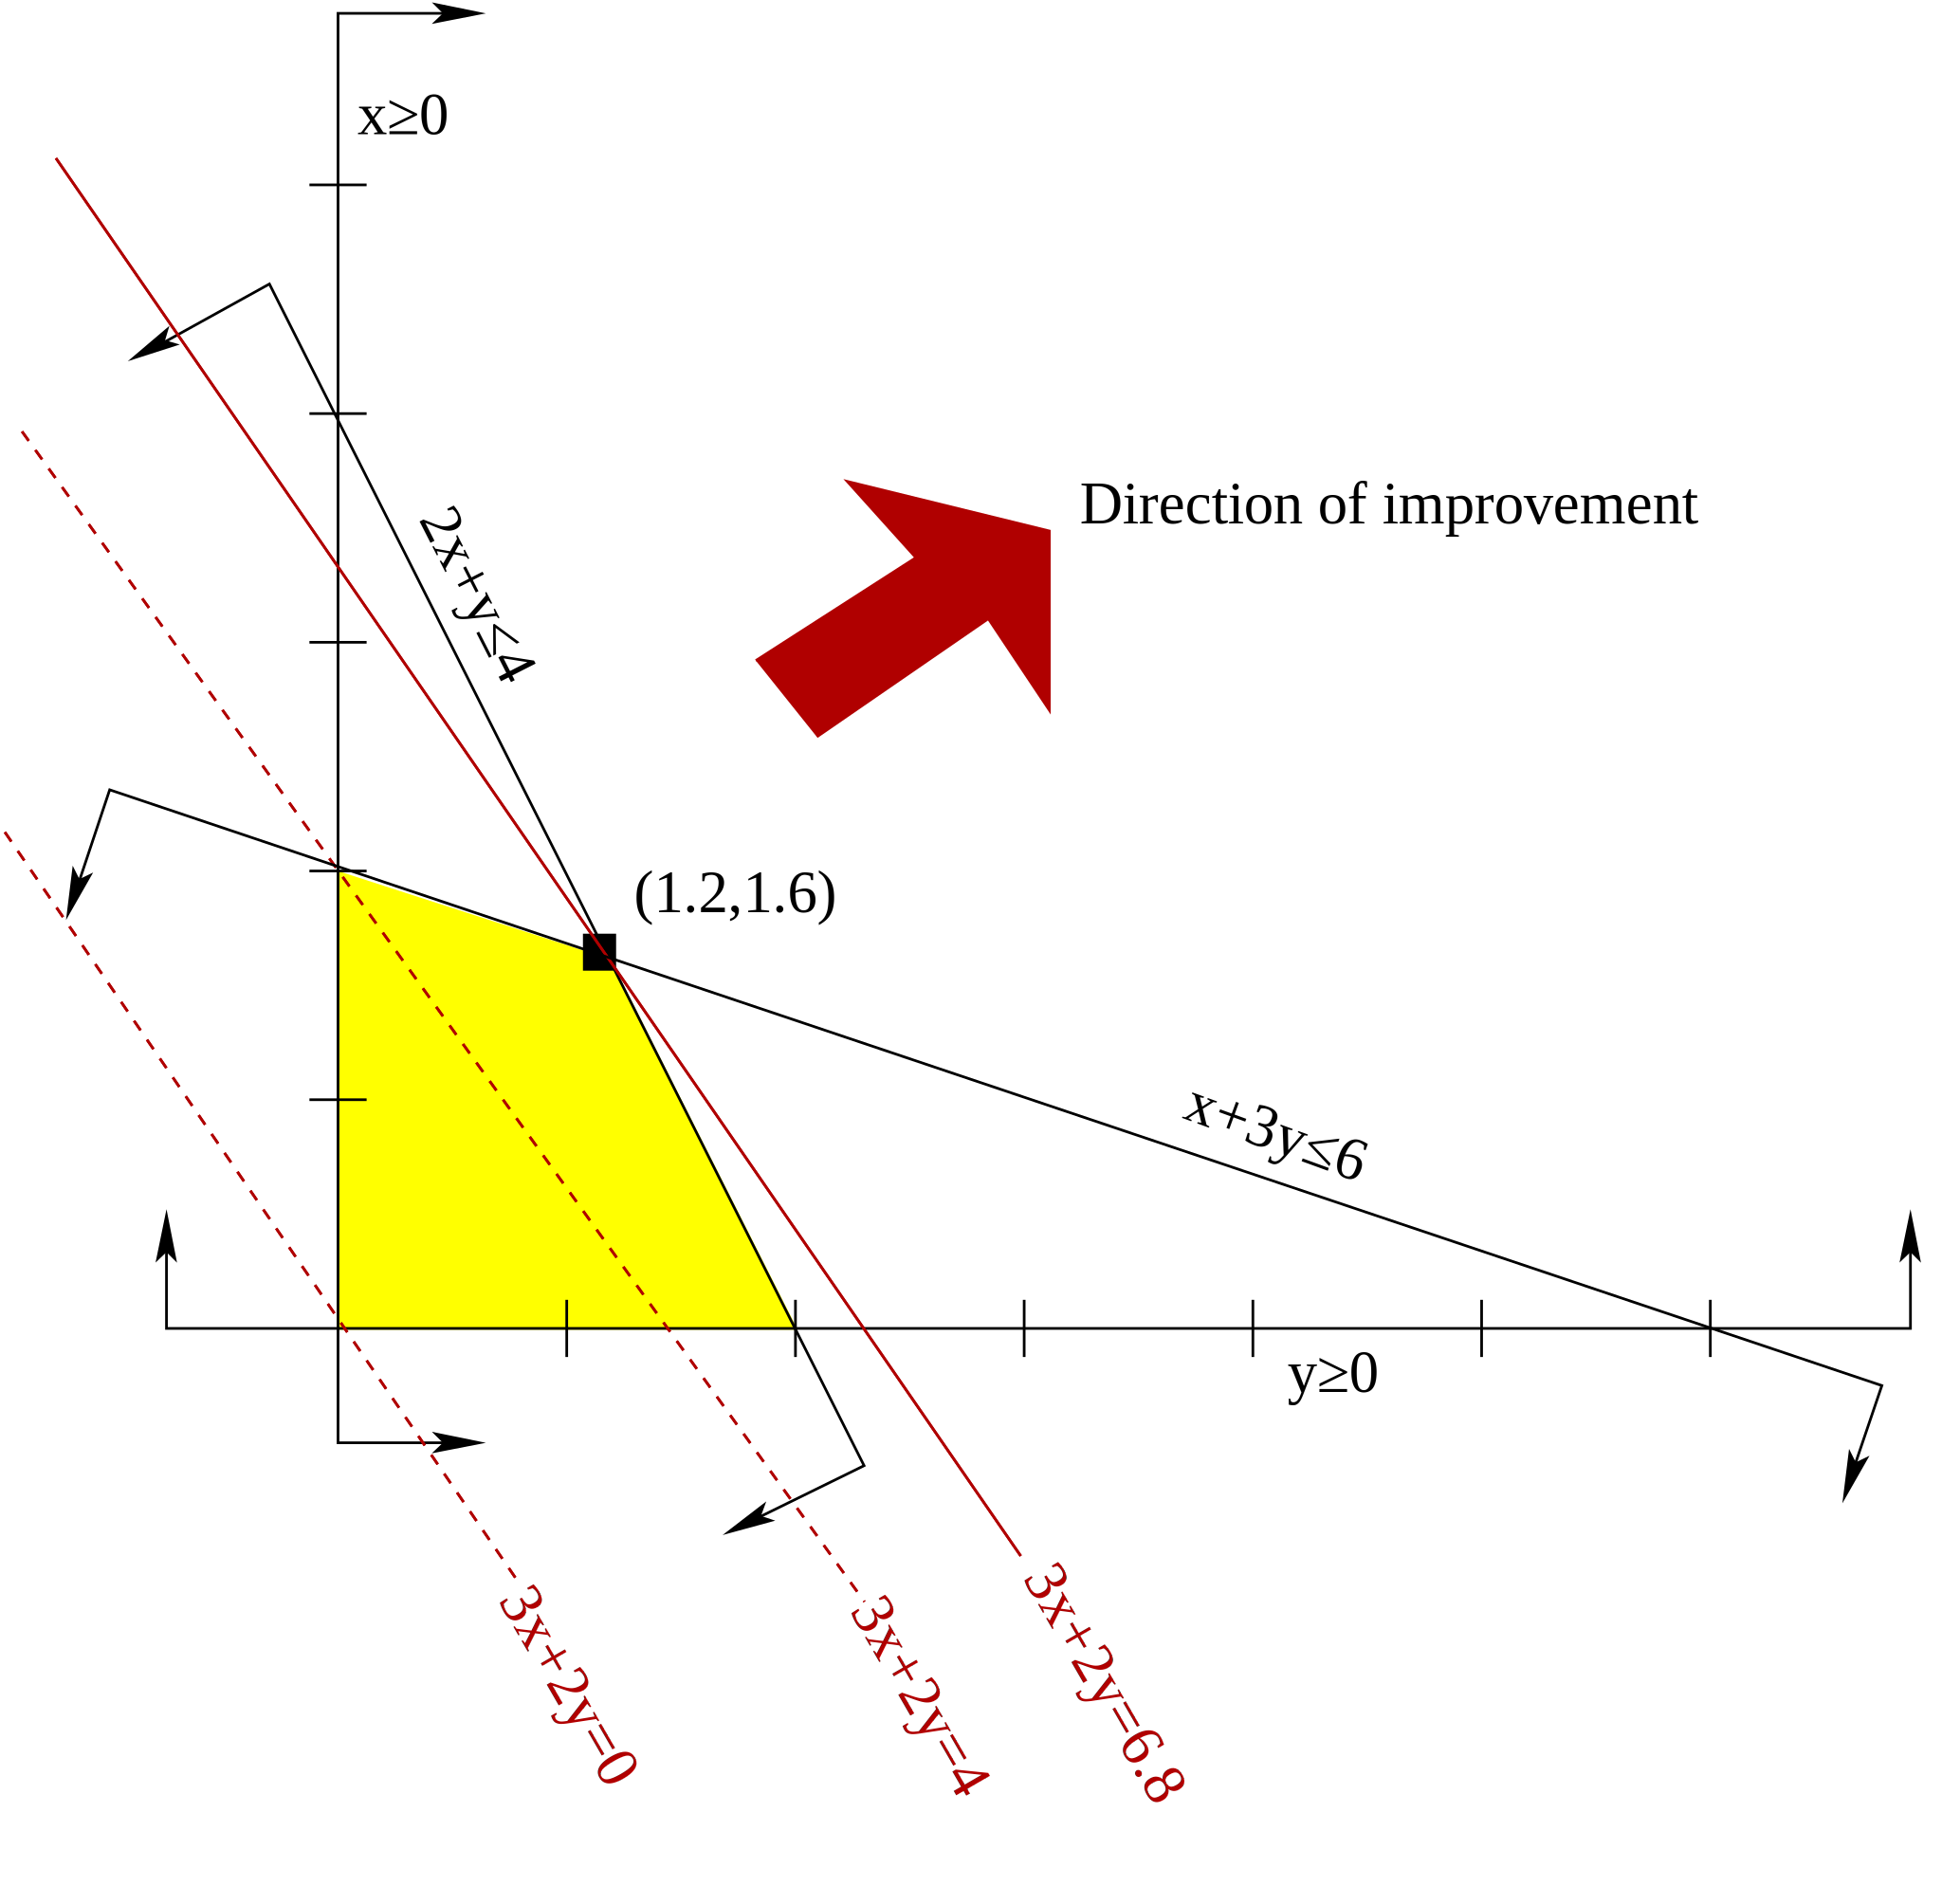
\includegraphics[width=0.8\linewidth]{images/lemon} \end{center}

In the figure above, the lines with \(z\) at 0, 4 and 6.8 have been
drawn. From the picture, we can see that if \(z\) is greater than 6.8,
the line defined by \(3x+2y = z\) will not intersect the feasible
region. Hence, the profit cannot exceed 6.8 dollars.

As the line \(3x+2y = 6.8\) does intersect the feasible region, \(6.8\)
is the maximum value for the objective function. Note that there is only
one point in the feasible region that intersects the line \(3x+2y=6.8\),
namely
\(\begin{bmatrix} x \\ y\end{bmatrix} = \begin{bmatrix} 1.2 \\ 1.6\end{bmatrix}.\)
In other words, to maximize profit, we want to make 1.2 units of
lemonade and 1.6 units of lemon juice.

The above solution method can hardly be regarded as rigorous because we
relied on a picture to conclude that \(3x + 2y \leq 6.8\) for all
\(\begin{bmatrix} x\\y\end{bmatrix}\) satisfying the constraints. But we
can actually show this \emph{algebraically}.

Note that multiplying both sides of the constraint \(x + 3y \leq 6\)
gives \(0.2x + 0.6 y \leq 1.2\), and multiplying both sides of the
constraint \(2x + y \leq 4\) gives \(2.8x + 1.4 y \leq 5.6\). Hence, any
\(\begin{bmatrix} x\\y\end{bmatrix}\) that satisfies both \(x+3y\leq 6\)
and \(2x+y \leq 4\) must also satisfy
\((0.2x+0.6y) + (2.8x+1.4y) \leq 1.2 + 5.6\), which simplifies to
\(3x + 2y \leq 6.8\) as desired! (Here, we used the fact that if
\(a \leq b\) and \(c \leq d\), then \(a+c \leq b+d\).)

Now, one might ask if it is always possible to find an algebraic proof
like the one above for similar problems. If the answer is yes, how does
one find such a proof? We will see answers to this question later on.

Before we end this segment, let us consider the following problem:
\[\begin{array}{rrcrll}
\mbox{minimize } & -2x & + & y & \\
\mbox{subject to} & -x & + & y & \leq & 3 \\
& x & - &  2y & \leq & 2 \\
& x &  & & \geq & 0 \\
& & & y & \geq & 0. \\
\end{array}\]

Note that for any \(t \geq 0\),
\(\begin{bmatrix} x \\ y\end{bmatrix} = \begin{bmatrix} t \\ t\end{bmatrix}\)
satisfies all the constraints. The value of the objective function at
\(\begin{bmatrix} x \\ y\end{bmatrix} = \begin{bmatrix} t \\ t\end{bmatrix}\)
is \(-t\). As \(t \rightarrow \infty\), the value of the objective
function tends to \(-\infty\). Therefore, there is no minimum value for
the objective function. The problem is said to be unbounded. Later on,
we will see how to detect unboundedness algorithmically.

As an exercise, check that unboundedness can also be established by
using
\(\begin{bmatrix} x \\ y\end{bmatrix} = \begin{bmatrix} 2t+2 \\ t\end{bmatrix}\)
for \(t \geq 0\).

\subsection*{Exercises}\label{exercises}
\addcontentsline{toc}{section}{Exercises}

\begin{enumerate}
\def\labelenumi{\arabic{enumi}.}
\item
  Sketch all \(\begin{bmatrix} x \\ y \end{bmatrix}\) satisfying

  \begin{equation*}
  x - 2y \leq 2
  \end{equation*}

  on the \((x,y)\)-plane.
\item
  Determine the optimal value of \[
  \begin{array}{rl}
  \text{Minimize} & x + y \\
  \text{Subject to} &  2x + y \geq 4 \\
  & x + 3y \geq 1.
  \end{array}
  \]
\item
  Show that the problem \[
  \begin{array}{rl}
  \text{Minimize} & -x + y \\
  \text{Subject to} &  2x - y \geq 0 \\
  & x + 3y \geq 3
  \end{array}
  \] is unbounded.
\item
  Suppose that you are shopping for dietary supplements to satisfy your
  required daily intake of 0.40mg of nutrient \(M\) and 0.30mg of
  nutrient \(N\). There are three popular products on the market. The
  costs and the amounts of the two nutrients are given in the following
  table:

  \begin{longtable}[]{@{}lccc@{}}
  \toprule
  & Product 1 & Product 2 & Product 3\tabularnewline
  \midrule
  \endhead
  Cost & \$27 & \$31 & \$24\tabularnewline
  Daily amount of \(M\) & 0.16 mg & 0.21 mg & 0.11 mg\tabularnewline
  Daily amount of \(N\) & 0.19 mg & 0.13 mg & 0.15 mg\tabularnewline
  \bottomrule
  \end{longtable}

  You want to determine how much of each product you should buy so that
  the daily intake requirements of the two nutrients are satisfied at
  minimum cost. Formulate your problem as a linear programming problem,
  assuming that you can buy a fractional number of each product.
\end{enumerate}

\subsection*{Solutions}\label{solutions}
\addcontentsline{toc}{subsection}{Solutions}

\begin{enumerate}
\def\labelenumi{\arabic{enumi}.}
\item
  The points \((x,y)\) satisfying \(x-2y \leq 2\) are precisely those
  above the line passing through \((2,0)\) and \((0,-1)\).
\item
  We want to determine the minimum value \(z\) so that \(x+y=z\) defines
  a line that has a nonempty intersection with the feasible region.
  However, we can avoid referring to a sketch by setting \(x=z-y\) and
  substituting for \(x\) in the inequalities to obtain:

  \begin{eqnarray*}
   2(z-y) + y \geq 4 \\
   (z-y) + 3y \geq 1,
  \end{eqnarray*}

  or equivalently,

  \begin{eqnarray*}
   z \geq 2+\frac{1}{2}y \\
   z \geq 1-2y,
  \end{eqnarray*}

  Thus, the minimum value for \(z\) is
  \(\min \{ 2+\frac{1}{2}y, 1-2y\}\), which occurs at
  \(y = -\frac{2}{5}\). Hence, the optimal value is \(\frac{9}{5}\).

  We can verify our work by doing the following. If our calculations
  above are correct, then an optimal solution is given by
  \(x = \frac{11}{5}\), \(y = -\frac{2}{5}\) since \(x = z - y\). It is
  easy to check that this satisfies both inequalities and therefore is a
  feasible solution.

  Now, taking \(\frac{2}{5}\) times the first inequality and
  \(\frac{1}{5}\) times the second inequality, we can infer the
  inequality \(x+y \geq \frac{9}{5}\). The left-hand side of this
  inequality is precisely the objective function. Hence, no feasible
  solution can have objective function value less than \(\frac{9}{5}\).
  But \(x = \frac{11}{5}\), \(y = -\frac{2}{5}\) is a feasible solution
  with objective function value equal to \(\frac{9}{5}\). As a result,
  it must be an optimal solution.

  \textbf{Remark.} We have not yet discussed how to obtain the
  multipliers \(\frac{2}{5}\) and \(\frac{1}{5}\) for inferring the
  inequality \(x+y \geq \frac{9}{5}\). This is an issue that will be
  taken up later. In the meantime, think about how one could have
  obtained these multipliers for this particular exercise.
\item
  We could glean some insight by first making a sketch on the
  \((x,y)\)-plane.

  The line defined by \(-x + y = z\) has \(x\)-intercept \(-z\). Note
  that for \(z \leq -3\),
  \(\begin{bmatrix} x\\y \end{bmatrix} = \begin{bmatrix} -z\\ 0\end{bmatrix}\)
  satisfies both inequalities and the value of the objective function at
  \(\begin{bmatrix} x\\y \end{bmatrix} = \begin{bmatrix} -z\\ 0\end{bmatrix}\)
  is \(z\). Hence, there is no lower bound on the value of objective
  function.
\item
  Let \(x_i\) denote the amount of Product \(i\) to buy for
  \(i = 1,2,3\). Then, the problem can be formulated as
  \[\begin{array}{rrcrcrll}
  \mbox{minimize } & 27 x_1 & + & 31 x_2 & + & 24 x_3 \\
  \mbox{subject to} 
  & 0.16 x_1 & + & 0.21 x_2 & + & 0.11 x_3 & \geq & 0.30 \\
  & 0.19 x_1 & + & 0.13 x_2 & + & 0.15 x_3 & \geq & 0.40 \\
  & x_1 & , & x_2 & , & x_3 & \geq & 0. \\
  \end{array}\]

  \textbf{Remark.} If one cannot buy fractional amounts of the products,
  the problem can be formulated as \[\begin{array}{rrcrcrll}
  \mbox{minimize } & 27 x_1 & + & 31 x_2 & + & 24 x_3 \\
  \mbox{subject to} 
  & 0.16 x_1 & + & 0.21 x_2 & + & 0.11 x_3 & \geq & 0.30 \\
  & 0.19 x_1 & + & 0.13 x_2 & + & 0.15 x_3 & \geq & 0.40 \\
  & x_1 & , & x_2 & , & x_3 & \geq & 0. \\
  & x_1 & , & x_2 & , & x_3 & \in & \mathbb{Z}. \\
  \end{array}\]
\end{enumerate}


\begin{tikzpicture}
    \draw[gray!50, thin, step=0.5] (-1,-3) grid (5,4);
    \draw[very thick,->] (-1,0) -- (5.2,0) node[right] {$x_1$};
    \draw[very thick,->] (0,-3) -- (0,4.2) node[above] {$x_2$};

    \foreach \x in {-1,...,5} \draw (\x,0.05) -- (\x,-0.05) node[below] {\tiny\x};
    \foreach \y in {-3,...,4} \draw (-0.05,\y) -- (0.05,\y) node[right] {\tiny\y};

    \fill[blue!50!cyan,opacity=0.3] (8/3,1/3) -- (1,2) -- (13/3,11/3) -- cycle;

    \draw (-1,4) -- node[below,sloped] {\tiny$x_1+x_2\geq3$} (5,-2);
    \draw (1,-3) -- (3,1) -- node[below left,sloped] {\tiny$2x_1-x_2\leq5$} (4.5,4);
    \draw (-1,1) -- node[above,sloped] {\tiny$-x_1+2x_2\leq3$} (5,4);

\end{tikzpicture}\footnote{
\url{https://tex.stackexchange.com/questions/75933/how-to-draw-the-region-of-inequality}
}

\fi

%\newcommand\oldstuff{thus}
%
\section{The Simplex Method} {The Simplex Method}
\todoSection{Integrate this to next chapter (chapter on simplex method)}
\label{lab:Simplex}
\objective{
The \emph{Simplex Method} is a straightforward algorithm for finding optimal solutions to optimization problems with linear constraints and cost functions.
Because of its simplicity and applicability, this algorithm has been named one of the most important algorithms invented within the last 100 years.
In this lab we implement a standard Simplex solver for the primal problem. %s that are feasible at the origin.
}

% The algorithm obtains the solution by traversing the edges of the feasible region defined by the constraints.
% The theory of convex optimization guarantees that the optimal point will be found among the vertices of the feasible region, and so a carefully implemented Simplex Algorithm will discover the exact solution in a finite number of steps.

\subsection*{Standard Form} % ====================================================

The Simplex Algorithm accepts a linear constrained optimization problem, also called a \emph{linear program}, in the form given below:

\begin{align*}
\text{minimize}\qquad &\c\trp\x \\
\text{subject to}\qquad & A\x \leq \b \\
 &\x \geq \0
\end{align*}

Note that any linear program can be converted to standard form, so there is no loss of generality in restricting our attention to this particular formulation.

Such an optimization problem defines a region in space called the \emph{feasible region}, the set of points satisfying the constraints.
Because the constraints are all linear, the feasible region forms a geometric object called a \emph{polytope}, having flat faces and edges (see Figure \ref{fig:polytope}).
The Simplex Algorithm jumps among the vertices of the feasible region searching for an optimal point.
It does this by moving along the edges of the feasible region in such a way that the objective function is always increased after each move.

\begin{figure}[H]
\captionsetup[subfigure]{justification=centering}
\centering
\begin{subfigure}{.5\textwidth} % 2-d feasible polytope.
    \centering
    \includegraphics[width=\linewidth]{foundationsAppliedMathematicsLabs/Volume2/Simplex/figures/feasiblePolytope.pdf}
    \caption{The feasible region for a linear program with 2-dimensional constraints.}
\end{subfigure}%
\begin{subfigure}{.5\textwidth} % 3-d feasible polytope.
    \begin{center}
    \begin{tikzpicture}[dot/.style={circle,fill=blue,minimum size=3pt,inner sep=0pt, outer sep=-1pt}, >=stealth']

    \draw[blue!10!, fill=blue!5!](3,1)--(1.5,2.3)--(1.75,1.3)--cycle;
    \draw[blue!25!, fill = blue!15!](3,1)--(1.75,1.3)--(2.3,-1)--cycle;
    \draw[blue!55!, fill = blue!40!](1.75,1.3)--(2.3,-1)--(.8,-1)--cycle;
    \draw[blue!80!, fill = blue!65!](.8,-1)--(-.05,-.2)--(.25,.6)--(1.22,.06)--cycle;
    \draw[blue!85!, fill = blue!73!](-.05, -.2)--(-.3,0)--(.1, 1.65)--(.25, .6)--cycle;
    \draw[blue!65!, fill = blue!50!](.1,1.7)--(.25,.6)--(1.22,.07)--(1.75,1.3)--cycle;
    \draw[blue!40!, fill = blue!15!](.1,1.7)--(1.75,1.3)--(1.5,2.3)--cycle;

    \draw[-,thick](-.3,0)--(.1,1.7)--(1.5, 2.3)--(3, 1)--(2.3,-1)--(.8,-1)--cycle;

    \draw[-,thick](.1,1.7)--(3,1);
    \draw[-,thick](1.5, 2.3)--(2.3,-1);
    \draw[-,thick](.8,-1)--(1.74,1.3);
    \draw[-,thick](.1,1.7)--(.25,.6);
    \draw[-,thick](1.24,.07)--(.25,.6);
    \draw[-,thick](-.05,-.24)--(.25,.6);

    \draw[->](.37,.63)--(.22,1.61);
    \draw[->](.31,1.55)--(1.63,1.23);
    \draw[->](.75,-.85)--(1.12,.05);
    \draw[->](1.05,.05)--(.25,.48);
    \draw[->](1.83,1.35)--(1.65,2.1);

    \node[draw=none](x*)at(1.8,2.45){$\x^*$};

    \end{tikzpicture}
    \end{center}
    \caption{The feasible region for a linear program with 3-dimensional constraints.}
\end{subfigure}
\caption{If an optimal point exists, it is one of the vertices of the polyhedron.
The simplex algorithm searches for optimal points by moving between adjacent vertices in a direction that increases the value of the objective function until it finds an optimal vertex.}
\label{fig:polytope}
\end{figure}

% \begin{figure}[htb] % 3-d feasible polytope.
% \end{figure}


% % TODO: subfigure for 3-d polytope from book.

Implementing the Simplex Algorithm is straightforward, provided one carefully follows the procedure.
We will break the algorithm into several small steps, and write a function to perform each one.
To become familiar with the execution of the Simplex algorithm, it is helpful to work several examples by hand.

\subsection*{The Simplex Solver} % ===============================================

Our program will be more lengthy than many other lab exercises and will consist of a collection of functions working together to produce a final result.
It is important to clearly define the task of each function and how all the functions will work together.
If this program is written haphazardly, it will be much longer and more difficult to read than it needs to be.
We will walk you through the steps of implementing the Simplex Algorithm as a Python class.
% Since the Simplex Algorithm assumes that all the variables are non-negative, we do not need any special logic for it.
% what is this previous statement saying? What 'special logic' would you need if the variables were negative?

For demonstration purposes, we will use the following linear program.
\begin{align*}
\text{minimize}\qquad & -3x_0 - 2x_1 \\
\text{subject to}\qquad
& x_0 - x_1 \leq 2 \\
& 3x_0 + x_1 \leq 5 \\
& 4x_0 + 3x_1 \leq 7 \\
& x_0, x_1 \geq 0.
\end{align*}

\subsection*{Accepting a Linear Program} % ------------------------------------

Our first task is to determine if we can even use the Simplex algorithm.
Assuming that the problem is presented to us in standard form, we need to check that the feasible region includes the origin.  For now, we only check for feasibility at the origin. A more robust solver sets up the auxiliary problem and solves it to find a starting point if the origin is infeasible.

\begin{problem}{Check feasibility at the origin.}{}
Write a class that accepts the arrays $\c$, $A$, and $\b$ of a linear optimization problem in standard form.
In the constructor, check that the system is feasible at the origin.
That is, check that $A\x \preceq \b$ when $\x = \0$. Raise a \li{ValueError} if the problem is not feasible at the origin. \label{prob:initsolver}
\end{problem}

\subsection*{Adding Slack Variables} % ----------------------------------------

The next step is to convert the inequality constraints $A\x \leq \b$ into equality constraints by introducing a slack variable for each constraint equation.
If the constraint matrix $A$ is an $m \times n$ matrix, then there are $m$ slack variables, one for each row of $A$.
Grouping all of the slack variables into a vector $\w$ of length $m$, the constraints now take the form $A\x + \w = \b$.
In our example, we have \[\w = \left[\begin{array}{c}x_2\\x_3 \\x_4\end{array}\right]\]

% TODO: change the representation of the slack variables to match the book.
When adding slack variables, it is useful to represent all of your variables, both the original primal variables and the additional slack variables, in a convenient manner.
One effective way is to refer to a variable by its subscript.
For example, we can use the integers $0$ through $n-1$ to refer to the original (non-slack) variables $x_0$ through $x_{n-1}$, and we can use the integers $n$ through $n+m-1$ to track the slack variables (where the slack variable corresponding to the $i$th row of the constraint matrix is represented by the index $n+i-1$).

We also need some way to track which variables are \emph{independent} (non-zero) and which variables are \emph{dependent} (those that have value $0$). This can be done using the objective function. At anytime during the optimization process, the non-zero variables in the objective function are \emph{independent} and all other variables are \emph{dependent}. 

%A useful representation for the variables is a Python list (or NumPy array), where the elements of the list are integers.
%Since we know how many dependent variables we have ($m$), we can partition the list so that all the dependent variables are kept in the first $m$ locations, and all the independent variables are stored at the end of the list.
%The ordering of this list is important.
%In particular, if $i \leq m$, the $i$th element of the list represents the dependent variable corresponding to the $i$th row of $A$.
%Henceforth we will refer to this list as the \emph{index list}.

%Initially, the dependent variables are simply the slack variables, and their values correspond to the values of %the vector $\b$.
%In our example, we have 2 primal variables $x_0$ and $x_1$, and we must add 3 slack variables.
%Thus, we instantiate the following index list:

%\begin{lstlisting}
%>>> L = [2, 3, 4, 0, 1]
%\end{lstlisting}

%Notice how the first $3$ entries of the index list are $2, 3, 4$, the indices representing the slack variables.
%This reflects the fact that the dependent variables at this point are exactly the slack variables.

%As the Simplex Algorithm progresses, however, the dependent variables change, and it will be necessary to swap
%elements in our index list.
%For example, suppose the variable represented by the index $4$ becomes independent, while the variable %represented by index $0$ becomes dependent.
%In this case we swap these two entries in the index list.

%\begin{lstlisting}
%>>> L[2], L[3] = L[3], L[2]
%>>> L
%[2, 3, 0, 4, 1]
%\end{lstlisting}

%Now our index list tells us that the current dependent variables $2, 3, 0$.

%\begin{problem} % Slack variables. % TODO: this problem is worthless...
%Design and implement a way to store and track all of the dependent and independent variables.

%Hint: Using integers that represent the index of each variable is useful for Problem \ref{prob:blands}.
%\label{prob:slackvars}
%\end{problem}

\subsection*{Creating a Dictionary} % --------------------------------------------

After we have determined that our program is feasible, we need to create the \emph{dictionary} (sometimes called the \emph{tableau}), a matrix to track the state of the algorithm.
%Remember that your dictionary will need to include in some way the slack variables that you created in Problem \ref{prob:slackvars}.

There are many different ways to build your dictionary.
One way is to mimic the dictionary that is often used when performing the Simplex Algorithm by hand. To do this we will set the corresponding dependent variable equations to 0. For example, if $x_5$ were a dependent variable we would expect to see a -1 in the column that represents $x_5$.
Define \[\bar{A} = \left[\begin{array}{cc} A & I_m \end{array}\right],\]
where $I_m$ is the $m \times m$ identity matrix we will use to represent our slack variables, and define
\[\bar{\c} = \left[\begin{array}{c}\c\\ \0\end{array}\right].\]
That is, $\bar{\c} \in \mathbb{R}^{n+m}$ such that the first $n$ entries are $\c$ and the final $m$ entries are zeros.
Then the initial dictionary has the form
\begin{equation}
D =
\left[\begin{array}{ccc}
0  & \bar{\c}\trp \\
\b &  -\bar{A} 
\end{array}\right]
\label{eqn:hand_tab}
\end{equation}

The columns of the dictionary correspond to each of the variables (both primal and slack), and the rows of the dictionary correspond to the dependent variables.
%Using the convention introduced above of representing the variables by indices in the index list, we have the following correspondence:
%\[
%\text{column } i \Leftrightarrow \text{index } i-2, \qquad i = 2, 3, \ldots, n+m+1,
%\]
%and
%\[
%\text{row } j \Leftrightarrow L_{j-1}, \qquad j = 2, 3, \ldots, m+1,
%\]
%where $L_{j-1}$ refers to the $(j-1)$th entry of the index list.

%For our example problem, the initial index list is
%\[
%L = (2, 3, 4, 0, 1),
%\]
For our example the initial dictionary is
\begin{equation*}
D = \begin{bmatrix}
    0 & -3 & -2 & 0 & 0 & 0\\
    2 & -1 & 1 & -1 & 0 & 0\\
    5 & -3 & -1 & 0 & -1 & 0\\
    7 & -4 & -3 & 0 & 0 & -1
    \end{bmatrix}.
\end{equation*}
%The third column corresponds to index $1$, and the fourth row corresponds to index $4$, since this is the
%third entry of the index list.

The advantage of using this kind of dictionary is that it is easy to check the progress of your algorithm by hand.
%The disadvantage is that pivot operations require careful bookkeeping to track the variables and constraints.

% This dictionary is less intuitive, and I think could lead to more confusion.
\begin{comment}
We can also use a dictionary of the format:
\begin{equation}
T = \begin{bmatrix}
    0 & \c\trp  & 0 \\
    \0 & I_n & \0\\
    \b & -A  & \0
\end{bmatrix}.
\label{eqn:matrix_tab}
\end{equation}
Here, $T$ is a square matrix of size $(n+m+1) \times (n+m+1)$.
The advantage of this form of the dictionary is that all the pivot bookkeeping is built into the matrix.
For our example problem, the initial dictionary of this form is
\begin{equation}
T = \begin{bmatrix}
        0 & 3 & 2 & 0 & 0 & 0 \\
        0 & 1 & 0 & 0 & 0 & 0 \\
        0 & 0 & 1 & 0 & 0 & 0 \\
        2 &-1 & 1 & 0 & 0 & 0 \\
        5 &-3 &-1 & 0 & 0 & 0 \\
        7 &-4 &-3 & 0 & 0 & 0
\end{bmatrix}.
\label{eqn:matrix_inittab}
\end{equation}
\end{comment}

\begin{problem}{Initialize the dictionary.}
Add a method to your Simplex solver that takes in arrays c, A, and b to create the initial dictionary (D) as a NumPy array.
\label{prob:makedictionary}
\end{problem}

\subsection{Pivoting} % ------------------------------------------------------

Pivoting is the mechanism that really makes Simplex useful.
Pivoting refers to the act of swapping dependent and independent variables, and transforming the dictionary appropriately.
This has the effect of moving from one vertex of the feasible polytope to another vertex in a way that increases the value of the objective function.
Depending on how you store your variables, you may need to modify a few different parts of your solver to reflect this swapping.

When initiating a pivot, you need to determine which variables will be swapped.
In the dictionary representation, you first find a specific element on which to pivot, and the row and column that contain the pivot element correspond to the variables that need to be swapped.
Row operations are then performed on the dictionary so that the pivot column becomes a negative elementary vector.

Let's break it down, starting with the pivot selection.
We need to use some care when choosing the pivot element.
To find the pivot column, search from left to right along the top row of the dictionary (ignoring the first column), and stop once you encounter the first negative value.
The index corresponding to this column will be designated the \emph{entering index}, since after the full pivot operation, it will enter
the basis and become a dependent variable.

Using our initial dictionary $D$ in the example, we stop at the second column:
\[ D = \left[ \:
\begin{array}{*{7}{c}}
\cline{2-2}
0 & \multicolumn{1}{|c}{-3} & \multicolumn{1}{|c}{-2} & 0 & 0 & 0\\
2 & \multicolumn{1}{|c}{-1} & \multicolumn{1}{|c}{1} & -1 & 0 & 0\\
5 & \multicolumn{1}{|c}{-3} & \multicolumn{1}{|c}{-1} & 0 & -1 & 0\\
7 & \multicolumn{1}{|c}{-4} & \multicolumn{1}{|c}{-3} & 0 & 0 & -1\\
\cline{2-2}
\end{array}
\right] \]
We now know that our pivot element will be found in the second column.
The entering index is thus $1$.

Next, we select the pivot element from among the negative entries in the pivot column (ignoring the entry in the first row).
\emph{If all entries in the pivot column are non-negative, the problem is unbounded and has no solution.}
In this case, the algorithm should terminate.
Otherwise, assuming our pivot column is the $j$th column of the dictionary and that the negative entries of this column are
$D_{i_1, j}, D_{i_2, j}, \ldots, D_{i_k, j}$, we calculate the ratios
\[
\frac{-D_{i_1,0}}{D_{i_1,j}}, \frac{-D_{i_2,0}}{D_{i_2,j}}, \ldots, \frac{-D_{i_k,0}}{D_{i_k,j}},
\]
and we choose our pivot element to be one that minimizes this ratio.
If multiple entries minimize the ratio, then we utilize \emph{Bland's Rule}, which instructs us to choose the entry in the row corresponding to the smallest index (obeying this rule is important, as it prevents the possibility of the algorithm cycling back on itself infinitely).
The index corresponding to the pivot row is designated as the \emph{leaving index}, since after the full pivot operation, it will leave the basis and become a independent variable.

In our example, we see that all entries in the pivot column (ignoring the entry in the first row, of course) are negative, and hence they are all potential choices for the pivot element.
We then calculate the ratios, and obtain
\[
\frac{-2}{-1} = 2,\quad \frac{-5}{-3} = 1.66...,\quad \frac{-7}{-4} = 1.75.
\]
We see that the entry in the third row minimizes these ratios.
Hence, the element in the second column (index 1), third row (index 2) is our designated
pivot element.

\[ D = \left[ \:
\begin{array}{*{7}{c}}

0 & -3 & -2 & 0 & 0 & 0\\
2 & -1 & 1 & -1 & 0 & 0\\\cline{2-2}
5 & \multicolumn{1}{|c}{-3} & \multicolumn{1}{|c}{-1} & 0 & -1 & 0\\\cline{2-2}
7 & -4 & -3 & 0 & 0 & -1\\
\end{array}
\right] \]

\begin{comment}
If we are using the dictionary representation in equation \ref{eqn:matrix_tab}, pivot operations are reduced to a simple matrix equation:
\[T = T + T_m \otimes T_n,\]
where $T_m$ is the column corresponding to the variable entering the basis and $T_n$ is a normalized vector corresponding to the variable leaving the basis.
The result of the equation is the new dictionary.

For example, for the initial dictionary, \ref{eqn:matrix_inittab}, we will demonstrate the first pivot operation.
We can do the entire pivot with a single outer product.
The first pivot should occur with $x_1$ leaving and $x_4$ entering.
In other words, we want to pivot at row $i = 4$ and column $j = 1$ in the dictionary (the indices are offset by one because of the objective function and the row of constraints).

The row corresponding to $x_4$ is
\[
\begin{bmatrix} 5 &-3 &-1 & 0 & 0 & 0\end{bmatrix}.
\]
This represents the equation
\[
x_4 = 5 - 3x_1 - x_2.
\]
Our eventual goal is to solve for $x_1$ and substitute into the remaining rows of the dictionary.
A simple method to accomplish this is to rewrite the equation so that we have zero on the left-hand side:
\[
0 = 5 - 3x_1 - x_2 - x_4.
\]
Now, we can normalize this equation so that the coefficient of $x_1$ is $-1$.
This is always accomplished by dividing the equation by the negative of the coefficient of $x_1$:
\begin{equation}
0 = \frac{5}{3} - x_1 - \frac{1}{3}x_2 - \frac{1}{3}x_4.
\label{eq:zero-equation}
\end{equation}
This is represented by the vector
\[
\begin{bmatrix} 5/3 & -1 & -1/3 & 0 & -1/3 & 0\end{bmatrix}.
\]
Since this left-hand side is zero, I can add any scalar multiple of this equation to any of the equations for $x_i$ and still have an equation for $x_i$.
For example, the equation for $x_5$ is
\[
x_5 = 7 - 4x_1 - 3x_2.
\]
Thus, I can add $-4$ times \eqref{eq:zero-equation} to this equation without changing the left-hand side:
\[ x_5 = 7 - 4x_1 - 3x_2 = 7 - 4x_1 - 3x_2 + -4\left(\frac{5}{3} - x_1 - \frac{1}{3}x_2 - \frac{1}{3}x_4\right) = \frac{1}{3} - \frac{5}{3}x_2 + \frac{4}{3} x_4.
\]
Notice that we end up with an equation that does not include $x_1$ and now has $x_4$, just like we wanted.
In fact, this works in all of our equations, including those for the objective function and even for $x_1$!
Since the coefficient of $x_1$ in \eqref{eq:zero-equation} is $-1$, when we scale it by the coefficient of $x_1$ in any particular row, the $x_1$ cancels out.
\[
T = T + \begin{bmatrix}3 \\ 1 \\ 0 \\ -1 \\ -3 \\ -4\end{bmatrix}\begin{bmatrix} 5/3 & -1 & -1/3 & 0 & -1/3 & 0\end{bmatrix}.
\]
The column vector is just the second column of $T$, which is the column containing the coefficients of $x_1$ in each row.
When we compute this sum, we obtain the dictionary.
\[
T = \begin{bmatrix}
        5 &  0 & 1 & 0 & -1 & 0 \\
        5/3 & 0 &-1/3 & 0 &-1/3 & 0 \\
        0 & 0 & 1 & 0 & 0 & 0 \\
        1/3 & 0 & 4/3 & 0 & 1/3 & 0 \\
        0 & 0 & 0 & 0 & 1 & 0 \\
        1/3 & 0 & -5/3 & 0 & 4/3 & 0
\end{bmatrix}.
\]
\end{comment}
%\begin{problem}
%Write a method that will determine the pivot row and pivot column according to Bland's Rule.
% \begin{comment}
\begin{definition}{Bland's Rule}
Choose the independent variable with the smallest index that has a negative coefficient in the objective function
as the leaving variable.
Choose the dependent variable with the smallest index among all the binding dependent variables.
\end{definition}

Bland's Rule is important in avoiding cycles when performing pivots.
This rule guarantees that a feasible Simplex problem will terminate in a finite number of pivots.% \emph{Hint:} Avoid dividing by zero.
% \end{comment}
%\label{prob:blands}
%\end{problem}

%The next step is to swap the entering and leaving indices in our index list.
%In the example, we determined above that these indices are $0$ and $3$.
%We swap these two elements in our index list,
%and the updated index list is now
%\[
%L = (2, 0, 4, 3, 1),
%\]
%so the dependent variables are now given by the indices $2, 0, 4$.

Finally, we perform row operations on our dictionary in the following way: divide the pivot row by the negative value of the pivot entry.
Then use the pivot row to zero out all entries in the pivot column above and below the pivot entry.
In our example, we first divide the pivot row by -3, and then zero out the two entries above the pivot element and the single entry below it:
\begin{align*}
\begin{bmatrix}
    0 & -3 & -2 & 0 & 0 & 0\\
    2 & -1 & 1 & -1 & 0 & 0\\
    5 & -3 & -1 & 0 & -1 & 0\\
    7 & -4 & -3 & 0 & 0 & -1
    \end{bmatrix} &\rightarrow
\begin{bmatrix}
    0 & -3 & -2 & 0 & 0 & 0\\
    2 & -1 & 1 & -1 & 0 & 0\\
    5/3 & -1 & -1/3 & 0 & -1/3 & 0\\
    7 & -4 & -3 & 0 & 0 & -1
    \end{bmatrix}\rightarrow\\
\begin{bmatrix}
    -5 & 0 & -1 & 0 & 1 & 0\\
    2 & -1 & 1 & -1 & 0 & 0\\
    5/3 & -1 & -1/3 & 0 & -1/3 & 0\\
    7 & -4 & -3 & 0 & 0 & -1
    \end{bmatrix} &\rightarrow
\begin{bmatrix}
    -5 & 0 & -1 & 0 & 1 & 0\\
    1/3 & 0 & -4/3 & 1 & -1/3 & 0\\
    5/3 & -1 & -1/3 & 0 & -1/3 & 0\\
    7 & -4 & -3 & 0 & 0 & -1
    \end{bmatrix}\rightarrow\\
\begin{bmatrix}
    -5 & 0 & -1 & 0 & 1 & 0\\
    1/3 & 0 & 4/3 & -1 & 1/3 & 0\\
    5/3 & -1 & -1/3 & 0 & -1/3 & 0\\
    1/3 & 0 & -5/3 & 0 & 4/3 & -1
    \end{bmatrix}&.
\end{align*}
The result of these row operations is our updated dictionary, and the pivot operation is complete.

\begin{problem}{Pivoting}
Add a method to your solver that checks for unboundedness and performs a single pivot operation from start to completion.
If the problem is unbounded, raise a \li{ValueError}.
\end{problem}

\vspace{2mm}

\subsection{Termination and Reading the Dictionary} % ---------------------------

Up to this point, our algorithm accepts a linear program, adds slack variables, and creates the initial dictionary.
After carrying out these initial steps, it then performs the pivoting operation iteratively until the optimal point is found.
But how do we determine when the optimal point is found? The answer is to look at the top row of the dictionary, which represents the objective function.
More specifically, before each pivoting operation, check whether all of the entries in the top row of the dictionary (ignoring the entry in the first column) are nonnegative.
If this is the case, then we have found an optimal solution, and so we terminate the algorithm.

The final step is to report the solution.
The ending state of the dictionary and index list tells us everything we need to know.
The minimal value attained by the objective function is found in the upper leftmost entry of the dictionary.
The dependent variables all have the value $0$ in the objective function or first row of our dictionary array. The independent variables have values given by the first column of the dictionary.
Specifically, the independent variable whose index is located at the $i$th entry of the index list has the value $T_{i+1, 0}$.

In our example, suppose that our algorithm terminates with the dictionary and index list in the following state:
\[
D = \begin{bmatrix}
-5.2 & 0 & 0 & 0 & 0.2 & 0.6\\
0.6 & 0 & 0 & -1 & 1.4 & -0.8\\
1.6 & -1 & 0 & 0 & -0.6 & 0.2\\
0.2 & 0 & -1 & 0 & 0.8 & -0.6\\
\end{bmatrix}
\]
%\[
%L = (2, 0, 1, 3, 4).
%\]
Then the minimal value of the objective function is $-5.2$.
The independent variables have indices $4, 5$ and have the value $0$.
The dependent variables have indices $3, 1,$ and $2$, and have values $.6, 1.6$, and $.2$, respectively.
In the notation of the original problem statement, the solution is given by
\begin{align*}
x_0 &= 1.6\\
x_1 &= .2.
\end{align*}

\begin{problem}{SimplexSolver.solve()}
Write an additional method in your solver called \li{solve()} that obtains the optimal solution, then returns the minimal value, the dependent variables, and the independent variables.
The dependent and independent variables should be represented as two dictionaries that map the index of the variable to its corresponding value.

For our example, we would return the tuple 

\li{(-5.2, \{0: 1.6, 1: .2, 2: .6\}, \{3: 0, 4: 0\})}.
%The correct format of this tuple is critical, as this tuple of information will be used judge whether or not your solver works!
\end{problem}

\vspace{5mm}

At this point, you should have a Simplex solver that is ready to use.
The following code demonstrates how your solver is expected to behave:

\vspace{5mm}

\begin{lstlisting}
>>> import SimplexSolver

# Initialize objective function and constraints.
>>> c = np.array([-3., -2.])
>>> b = np.array([2., 5, 7])
>>> A = np.array([[1., -1], [3, 1], [4, 3]])

# Instantiate the simplex solver, then solve the problem.
>>> solver = SimplexSolver(c, A, b)
>>> sol = solver.solve()
>>> print(sol)
(-5.2,
 {0: 1.6, 1: 0.2, 2: 0.6},
 {3: 0, 4: 0})
\end{lstlisting}

If the linear program were infeasible at the origin or unbounded, we would expect the solver to alert the user by raising an error.

Note that this simplex solver is \emph{not} fully operational.
It can't handle the case of infeasibility at the origin.
This can be fixed by adding methods to your class that solve the \emph{auxiliary problem}, that of finding an initial feasible dictionary when the problem is not feasible at the origin.
Solving the auxiliary problem involves pivoting operations identical to those you have already implemented, so adding this functionality
is not overly difficult.


\subsection{Exercises}

\paragraph{Exercise $1.0$ (Learn $\mathrm{LT}_{\mathrm{E}} \mathrm{X}$ )}

Learn to use $\operatorname{lt}_{\mathrm{E}} X$ for writing all of your homework solutions. Personally, I use MiKTEX, which is an implementation of $\mathrm{ET} \mathrm{E} \mathrm{X}$ for Windows. Specifically, within MiKTEX I am using pdfteTEX (it only matters for certain things like including graphics and also pdf into a document). I find it convenient to use the editor WinEdt, which is very LATEX friendly. A good book on $\mathrm{ET} \mathrm{T} \mathrm{X}$ is

In A.1 there is a template to get started. Also, there are plenty of tutorials and beginner's guides on the web.

\paragraph{Exercise $1.1$ (Convert to standard form)}

Give an original example (i.e., with actual numbers) to demonstrate that you know how to transform a general linear-optimization problem to one in standard form.

\paragraph{Exercise $1.2$ (Weak Duality example)}

Give an original example to demonstrate the Weak Duality Theorem.

\paragraph{Exercise $1.3$ (Convert to $\leq$ form)}

Describe a general recipe for transforming an arbitrary linear-optimization problem into one in which all of the linear constraints are of $\leq$ type.

\paragraph{Exercise $1.4$ ( $m+1$ inequalities)}

Prove that the system of $m$ equations in $n$ variables $A x=b$ is equivalent to the system $A x \leq b$ augmented by only one additional linear inequality - that is, a total of only $m+1$ inequalities.

\paragraph{Exercise $1.5$ (Weak duality for another form)}

Give and prove a Weak Duality Theorem for

$$
\begin{aligned}
\max \quad c^{\prime} x & \\
A x & \leq b ; \\
x & \geq 0 .
\end{aligned}
$$

HINT: Convert $\left(\mathrm{P}^{\prime}\right)$ to a standard-form problem, and then apply the ordinary Weak Duality Theorem for standard-form problems. \paragraph{Exercise 1.6 (Weak duality for a complicated form)}

Give and prove a Weak Duality Theorem for

$$
\begin{gathered}
\min \quad c^{\prime} x+f^{\prime} w \\
\begin{aligned}
A x+B w & \leq b ; \\
D x &=g ;
\end{aligned} \\
x \geq 0 \quad w \leq 0
\end{gathered}
$$

HINT: Convert $\left(\mathrm{P}^{\prime}\right)$ to a standard-form problem, and then apply the ordinary Weak Duality Theorem for standard-form problems.

\paragraph{Exercise $1.7$ (Weak duality for a complicated form - with MATLAB)}

The MATLAB code below makes and solves an instance of $\left(\mathrm{P}^{\prime}\right)$ from Exercise 1.6. Study the code to see how it is works. Now, extend the code to solve the dual of $\left(\mathrm{P}^{\prime}\right)$. Also, after converting $\left(\mathrm{P}^{\prime}\right)$ to standard form (as indicated in the HINT for Exercise 1.6), use MATLAB to solve that problem and its dual. Make sure that you get the same optimal value for all of these problems.





\subsection{$2.5$ Exercises}

\paragraph{Exercise 2.1 (Dual in AMPL)}

Without changing the file production. dat, use AMPL to solve the dual of the Production Problem example, as described in Section 2.1. You will need to modify production.mod and production.run.

\paragraph{Exercise $2.2$ (Sparse solution for linear equations with AMPL)}

In some application areas, it is interesting to find a "sparse solution" - that is, one with few non-zeros - to a system of equations $A x=b$. It is well known that a 1-norm minimizing solution is a good heuristic for finding a sparse solution. Using AMPL, try this idea out on several large examples, and report on your results.

HINT: To get an interesting example, try generating a random $m \times n$ matrix $A$ of zeros and ones, perhaps $m=50$ equations and $n=500$ variables, maybe with probability $1 / 2$ of an entry being equal to one. Then choose maybe $m / 2$ columns from $A$ and add them up to get $b$. In this way, you will know that there is a solution with only $m / 2$ non-zeros (which is already pretty sparse). Your 1-norm minimizing solution might in fact recover this solution $(\odot)$, or it may be sparser $(\odot \odot)$, or perhaps less sparse $(\odot)$.

\paragraph{Exercise $2.3$ (Bloody AMPL)}

A transportation problem is a special kind of (single-commodity min-cost) networkflow problem. There are certain nodes $v$ called supply nodes which have net supply $b_{v}>0$. The other nodes $v$ are called demand nodes, and they have net supply $b_{v}<0$. There are no nodes with $b_{v}=0$, and all arcs point from supply nodes to demand nodes.

A simplified example is for matching available supply and demand of blood, in types $A, B, A B$ and $O$. Suppose that we have $s_{v}$ units of blood available, in types $v \in\{A, B, A B, O\}$. Also, we have requirements $d_{v}$ by patients of different types $v \in$ $\{A, B, A B, O\}$. It is very important to understand that a patient of a certain type can accept blood not just from their own type. Do some research to find out the compatible blood types for a patient; don't make a mistake - lives depend on this! In this spirit, if your model misallocates any blood in an incompatible fashion, you will receive a grade of $F$ on this problem.

Describe a linear-optimization problem that satisfies all of the patient demand with compatible blood. You will find that type $O$ is the most versatile blood, then both $A$ and $B$, followed by $A B$. Factor in this point when you formulate your objective function, with the idea of having the left-over supply of blood being as versatile as possible.

Using AMPL, set up and solve an example of a blood-distribution problem.

\paragraph{Exercise $2.4$ (Mix it up)}

"I might sing a gospel song in Arabic or do something in Hebrew. I want to mix it up and do it differently than one might imagine." - Stevie Wonder

We are given a set of ingredients $1,2, \ldots, m$ with availabilities $b_{i}$ and per unit costs $c_{i}$. We are given a set of products $j, 2, \ldots, m$ with minimum production requirements $d_{j}$ and per unit revenues $e_{j}$. It is required that product $j$ have at least a fraction of $l_{i j}$ of ingredient $i$ and at most a fraction of $u_{i j}$ of ingredient $i$. The goal is to devise a plan to maximize net profit.

Formulate, mathematically, as a linear-optimization problem. Then, model with AMPL, make up some data, try some computations, and report on your results. Exercise $2.5$ (Task scheduling)


We are given a set of tasks, numbered $1,2, \ldots, n$ that should be completed in the minimum amount of time. For convenience, task 0 is a "start task" and task $n+1$ is an "end task". Each task, except for the start and end task, has a known duration $d_{i}$. For convenience, let $d_{0}:=0$. There are precedences between tasks. Specifically, $\Psi_{i}$ is the set of tasks that must be completed before task $i$ can be started. Let $t_{0}:=0$, and for all other tasks $i$, let $t_{i}$ be a decision variable representing its start time.

Formulate the problem, mathematically, as a linear-optimization problem. The objective should be to minimize the start time $t_{n+1}$ of the end task. Then, model the problem with AMPL, make up some data, try some computations, and report on your results.

\paragraph{Exercise $2.6$ (Investing wisely)}

Almost certainly, Albert Einstein did not say that "compound interest is the most powerful force in the universe."

A company wants to maximize their cash holdings after $T$ time periods. They have an external inflow of $p_{t}$ dollars at the start of time period $t$, for $t=1,2, \ldots, T$. At the start of each time period, available cash can be allocated to any of $K$ different investment vehicles (in any available non-negative amounts). Money allocated to investmentvehicle $k$ at the start of period $t$ must be held in that investment $k$ for all remaining time periods, and it generates income $v_{t, t}^{k}, v_{t, t+1}^{k}, \ldots, v_{t T}^{k}$, per dollar invested. It should be assumed that money obtained from cashing out the investment at the end of the planning horizon (that is, at the end of period $T$ ) is part of $v_{t, T}^{k}$. Note that at the start of time period $t$, the cash available is the external inflow of $p_{t}$, plus cash accumulated from all investment vehicles in prior periods that was not reinvested. Finally, assume that cash held over for one time period earns interest of $q$ percent.

Formulate the problem, mathematically, as a linear-optimization problem. Then, model the problem with AMPL, make up some data, try some computations, and report on your results.







\end{document}
